\documentclass[times, utf8, diplomski, numeric]{fer}
\usepackage{booktabs}
\usepackage{courier}
\usepackage{xcolor}
\usepackage{multicol}
\graphicspath{ {./slike/} }
\usepackage[parfill]{parskip}

% kod
\usepackage{listings}
\usepackage{pmboxdraw}

\lstset{literate= {├}{{\pmboxdrawuni{251C}}}1 
                  {│}{{\pmboxdrawuni{2502}}}1 
                  }

% \lstset{basicstyle=\footnotesize\ttfamily,breaklines=true}
\lstdefinestyle{stil}{
    %belowcaptionskip=1\baselineskip,
    breaklines=true,
    frame=single,
    numbers=left,
    basicstyle=\footnotesize\ttfamily,
    keywordstyle=\bfseries\color{green!40!black},
    commentstyle=\itshape\color{purple!40!black},
    identifierstyle=\color{blue},
    captionpos=b,
}

\lstdefinestyle{terminal}{
    %belowcaptionskip=1\baselineskip,
    breaklines=true,
    frame=single,
    numbers=left,
    basicstyle=\footnotesize\ttfamily,
    keywordstyle=\bfseries\color{black},
    commentstyle=\itshape\color{black},
    identifierstyle=\color{black},
    captionpos=b,
}
\lstset{style=stil}
\renewcommand{\lstlistingname}{Ispis}% Listing -> Ispis


% dodano za prekidanje URL-ova na / i -
\usepackage{url}
\def\UrlBreaks{\do\/\do-}


% prekidanje monospace rijeci na _
\newcommand*\ttvar[1]{\texttt{\expandafter\dottvar\detokenize{#1}\relax}}
\newcommand*\dottvar[1]{\ifx\relax#1\else
  \expandafter\ifx\string_#1\string_\allowbreak\else#1\fi
  \expandafter\dottvar\fi}

\begin{document}

\thesisnumber{656}

\title{Proširivi sustav za stvaranje CTF zadataka specifičnih za sustave upravljanja i
zabave u automobilima}

\author{Lovro Grgurić Mileusnić}

\maketitle

% Ispis stranice s napomenom o umetanju izvornika rada. Uklonite naredbu \izvornik ako želite izbaciti tu stranicu.
\izvornik

% Dodavanje zahvale ili prazne stranice. Ako ne želite dodati zahvalu, naredbu ostavite radi prazne stranice.
\zahvala{}

\tableofcontents

\chapter{Uvod}
Današnji automobili i ostala cestovna vozila značajno se razlikuju od njihovih prvih inačica, iako im glavna namjena ostala ista. Pojavom i širom primjenom elektronike, automobili više nisu samo mehanički strojevi, već sadrže određen broj međusobno povezanih elektroničkih upravljačkih jedinica (engl. \textit{electronic control unit}, ECU) \cite{koscher2010}. Elektroničke upravljačke jedinice svojom međusobnom suradnjom omogućavaju sigurno upravljanje vozilom, ali i dodatne funkcionalnosti poput klimatizacije te sustava za informacije i zabavu (engl. \textit{in-vehicle infotainment}). Većina komunikacije između elektroničkih upravljačkih jedinica odvija se putem protokola poput \textit{Controller Area Network} (CAN) protokola i pripadajućih sabirnica. Prvotno namijenjen za primjenu u automobilima, CAN ima svojstva prikladna za komunikaciju u stvarnom vremenu (engl. \textit{realtime}), kao i sposobnosti detektiranja grešaka i propuštanja poruka višeg prioriteta \cite{canopen1}. Međutim, iako ga specifikacija druge inačice CAN protokola, CAN 2.0, opisuje kao protokol s visokom razinom sigurnosti, ni ta niti originalna specifikacija ne razmatraju osiguravanje osnovnih sigurnosnih svojstava povjerljivosti, integriteta i dostupnosti (engl. \textit{confidentiality, integrity, availability}, CIA) \cite{bosch1991, canislabs1}. Zbog drastične prirode posljedica koje bi neispravan rad sustava automobila mogao imati na vozača i njegove suputnike te ostale sudionike prometa, pri inženjeringu sustava automobila uvijek je bila pridodana posebna pažnja njihovoj funkcionalnoj sigurnosti (engl. \textit{safety}) i ispravnosti, ali ne nužno i kibernetičkoj sigurnosti \cite{koscher2010}. Zbog tadašnje zatvorenosti komunikacije ovih sustava, za potencijalnog napadača nije postojala površina (engl. attack surface) koju bi mogao iskoristiti bez fizičkog pristupa CAN sabirnici.

Interne mreže današnjih vozila kao i programska podrška njihovih sustava znatno su kompleksnije i povezanije s vanjskim svijetom \cite{huq2020driving}. Mnogi novi modeli automobila su opremljeni SIM karticama odnosno mogućnošću povezivanja na mobilnu mrežu u svrhu komunikacije sa servisima proizvođača u oblaku (engl. cloud services) i mobilnim aplikacijama koje omogućuju udaljeno upravljanje vozilom. Uz nevedeno, mobilna mreža koristi se i u svrhu preuzimanja ažuriranja (engl. \textit{Over-The-Air updates}, OTA) za sustave zabave, ali i za kritične elektroničke upravljačke jedinice. \textit{Bluetooth} tehnologija najčešće se koristi za povezivanje mobilnog telefona sa sustavom zabave kako bi se omogućilo pozivanje i reprodukcija glazbe. U svrhu bolje integracije mobilnih telefona u sustav zabave, mnogi proizvođači podržavaju platforme poput \textit{Android Auto} ili \textit{Apple Carplay}, kojima se sustav zabave proširuje mogućnostima preuzimanja i pokretanja raznovrsnih aplikacija iz izvora treće strane. Vozila opremljena mrežnim karticama s mogućnošću stvaranja i korištenja Wi-Fi bežičnih pristupnih točaka, mogu dijeliti pristup mobilnoj mreži koji ostvaruju s prethodno navedenim SIM karticama ili povezivati se na pristupne točke korisnika u svrhu preuzimanja OTA ažuriranja ili aplikacija. Za skoro svaku od navedenih funkcionalnosti istraživači automobilske sigurnosti pokazali su mogućnost njihvog iskorištavanja i ulančavanja otkrivenih ranjivosti u svrhu neautoriziranog pristupa i postizanja kontrole nad sustavima zabave, ali i kritičnim sustavima upravljanja automobila \cite{tencent2017free, tencent2018over, tencent2019bmw, tencent2018bmw, miller2015remote, curry2023web}. Nadalje, već u izvješću o stanju automobilske sigurnosti tvrtke \textit{Upstream Security} iz 2019. godine, predviđa se da će sva nova vozila proizvedena u 2025. godini imati navedene funkcionalnosti, ali i da će podržavati komunikaciju među vozilima (engl. \textit{Vehicle-to-Vehicle, V2V}) i komunikaciju vozila s infrastrukturom (engl. \textit{Vehicle-to-Infrastructure, V2I}), dodatno povećavajući dostupnu površinu napada \cite{upstream2019report}.

Nagli rast povezanosti i kompleksnosti sustava vozila stvara potrebu za obrazovanjem određenog broja stručnjaka i inženjera koji će testirati i osiguravati kvalitetniju kibernetičku sigurnost tih sustava, od razine sklopovlja do \textit{backend} servisa te V2V i V2I komunikacije. Osim formalnih sustava obrazovanja, popularan format za edukaciju stručnjaka kibernetičke sigurnosti su i \textit{Capture the Flag} (CTF) zadaci. Međutim, u \cite{vsvabensky2021cybersecurity} autori ističu da se u analiziranom uzorku od 12 952 \textit{Capture the Flag} zadataka, zadaci klasificirani u područje sigurnosti komponenti (engl. \textit{component security}) čine tek 8,19\%, što je 6. najmanji udio od ukupno 8 analiziranih područja znanja. Većina današnjih \textit{Capture the Flag} zadataka spada u razvijenije i poznatije grane kibernetičke sigurnosti poput \textit{web} sigurnosti, sigurnosti operacijskih sustava i aplikacija te sigurnosti oblaka (engl. \textit{cloud security})\cite{prinetto2020hardware}. U svrhu edukacije sigurnosnih stručnjaka u području kibernetičke sigurnosti u automobilskoj industriji potrebno je napraviti proširivi sustav koji će služiti kao temelj za stvaranje \textit{Capture the Flag} zadataka koji sadrže specifičnosti sustava u automobilima.

Rad je strukturiran kroz 6 poglavlja. U prvom poglavlju nakon uvoda, odnosno drugom poglavlju cjelokupnog rada, napravljen je pregled protokola te arhitekture modernog automobila. Kroz ovo poglavlje opisani su protokoli i sustavi modernog automobila, čime se postavlja teoretska podloga za razumijevanje napada na iste, opisanih u trećem poglavlju. U četvrtom poglavlju razmatraju se postojeći sustavi za obuku stručnjaka sigurnosti u grani sigurnosti automobila i definiran je popis poželjnih svojstava takvog sustava. U petom poglavlju opisana je implementacija proširivog sustava za stvaranje \textit{Capture the Flag} zadataka specifičnih za sustave upravljanja i zabave u automobilima. U zaključku je opisan konačan rezultat, prednosti i nedostatci implementiranog sustava te moguća unaprjeđenja i smjernice za daljnji razvoj.

\chapter{Sustavi i protokoli modernih automobila}
Kao temelj za razumijevanje iskoristivih površina i mogućih vektora napada na sustave automobila, kroz ovo poglavlje opisana je električna i elektronička arhitektura modernog automobila (engl. \textit{Electrical/Electronic} architecture). Opisani su i protokoli specifični za automobile kroz više slojeva OSI modela.
\section{E/E arhitektura modernog automobila}
E/E arhitektura obuhvaća elektroničke komponente, električko ožičenje, tehnologije umrežvanja i programsku podršku jednog automobila \cite{nasser2023automotive}. Prema \cite{nasser2023automotive, koscher2010, knight2020hacking, huq2020driving, aliwa2021cyberattacks}, sustavi vozila dijele se prema funkciji u domene:

\begin{itemize}
    \item pogonskog sklopa (engl. \textit{powertrain})
    \item šasije (engl. \textit{chassis})
    \item kabine (engl. \textit{interior cabin} ili \textit{body})
    \bigskip
    \item zabave i povezivosti (engl. \textit{infotainment and connectivity})
\end{itemize}

Iako se sustavi mogu prema funkciji podijeliti u navedene 4 domene, domene nužno ne određuju topologiju mreže automobila.

Domene pogonskog sklopa, šasije i kabine sadrže ECU-ove koji najviše utječu na fizičko stanje automobila te je njihova komunikacija većinom ograničena na internu mrežu automobila. Domena informacija, zabave i povezivosti sadrži sustave koji pružaju dodatne informacije i sadržaje vozaču i putnicima te vrše komunikaciju i s okolinom automobila, primjerice s \textit{backend} servisima, mobilnim uređajima i aplikacijama. Stoga je domena informacija, zabave i povezivosti obrađena u zasebnom potpoglavlju.   
\subsection{Domene pogonskog sklopa, šasije i kabine}
Elektroničke upravljačke jedinice odnosno ECU-ovi, pripadaju domenama pogonskog sklopa, šasije i unutarnje kabine te služe za koordiniranje i upravljanje većinom funkcija automobila. ECU-ovi detektiraju trenutne operativne uvjete pomoću senzora, procesuiraju ih i aktiviraju aktuatore \cite{bosch2022handbook}. Sklopovlje ECU-a najčešće se nalazi u zatvorenom zaštitnom kućištu s izloženim priključcima za spajanje na ostatak mreže automobila, senzore i aktuatore. Sklopovlje je najčešće tiskana pločica na kojoj se najčešće nalazi integrirani krug za upravljanje snagom (engl. \textit{power management integrated circuit}, PMIC), primopredajnici protokola kojim komuniciraju, memorije te mikrokontroler ili sustav na čipu (engl. \textit{System on a chip}), SoC)\cite{nasser2023automotive}. ECU-ovi ovih domena najčešće zbog \textit{realtime} zahtjeva međusobno komuniciraju putem CAN ili FlexRay protokola, gdje specifična topologija mreže ovisi o modelu automobila \cite{bosch2022handbook}.

Domeni pogonskog sklopa pripadaju ECU-ovi koji upravljaju i utječu na funkciju motora i prijenosa, a to su upravljački modul motora (engl. \textit{engine control module}, ECM) i upravljački modul prijenosa (engl. \textit{transmission control module}, TCM). U literaturi se često koriste i nazivi upravljačka jedinica motora (engl. \textit{engine control unit}, ECU), odnosno upravljačka jedinica prijenosa (engl. \textit{transmission control unit}, TCU)\cite{nasser2023automotive, koscher2010}. Često automobili imaju jedan snažniji ECU koji obavlja obje funkcije, upravljanje motorom i upravljanje prijenosom te se takav ECU naziva upravljačkom jedinicom pogonskog sklopa (engl. \textit{powertrain control unit}, PCU) ili upravljačkim modulom pogonskog sklopa (engl. \textit{powertrain control module}, PCM) \cite{bosch2022handbook, ecutesting}. U slučaju vozila na električni pogon, u domeni pogonskog sklopa pripadaju sustav upravljanja baterijom (engl. \textit{battery managment system}, BMS), inverter \engl{inverter} i PCU. Uz navedene, u domenu pogonskog sklopa ulaze i druge upravljačke jedinice koje prikupljaju podatke sa senzora i upravljaju aktuatorima relevantnima pogonskom sklopu. S obzirom na to da navedeni ECU-ovi imaju izravan utjecaj na kretanje automobila, njihovo kompromitiranje može rezultirati fizičkim ozljedama vozača i putnika.

U domenu šasije svrstavaju se sustavi i senzori odgovorni za funkcije zaštite putnika koje zahtijevaju reakciju u stvarnom vremenu poput sustava kočenja, ovjesa i zračnih jastuka. Sukladno tome, kao i u slučaju sustava domene pogonskog sklopa, njihovo ispravno funkcioniranje je iznimno bitno za sigurnost vozača i putnika \cite{nasser2023automotive}. Jedna od upravljačkih jedinica koje pripadaju u domenu šasije je upravljački modul elektroničkog kočenja (engl. \textit{electronic braking control module}, EBCM). EBCM je specijalizirani modul koji upravlja aktivnim sigurnosnim mjerama poput ABS-a (njem. \textit{Antiblockiersystem}), elektroničkom kontrolom stabilnosti (engl. \textit{electronic stability control}, ESC) te automatskog hitnog kočenja (engl. \textit{automated emergency breaking}, AEB). Uz EBCM, u domenu šasije svrstavaju se i napredni sustav za podršku vozaču pri upravljanju vozilom (engl. \textit{Advanced driver-assistance system}, ADAS), koji je sve češće prisutan u novim vozilima \cite{nasser2023automotive}. ADAS je odgovoran za funkcije poput rada tempomata, održavanja razmaka između vozila,  automatskog zadržavanja trenutne prometne trake, automatskog parkiranja te autonomne vožnje \cite{bosch2022handbook}. Domeni šasije pripada i upravljački modul zračnih jastuka (engl. \textit{airbag control module}, ACM) te sustav servo upravljača (engl. \textit{electronic power steering}, EPS). ADAS i EBCM prikupljaju podatke od niza sustava senzora, primjerice od radara za određivanje udaljenost objekata u svrhu aktivacije funkcije AEB, od ultrazvučnih senzora za potrebe sustava automatskog parkiranja te od sustava lidar i video senzora za potrebe autonomne vožnje. 

U domenu kabine spadaju sustavi manje kritičnih funkcija te uključuju sustave grijanja, ventilacije i klimatizacije (engl. \textit{heating, ventilation and air conditioning}, HVAC), pripadajući upravljački modul klimatizacije (engl. \textit{climate control module}, CCM) te ECU-ove za prikupljanje podataka sa senzora sigurnosnih pojasa i sjedala te ECU-ove za upravljanje ambijentalnim osvjetljenjem, prozorima, brisačima i ostalim dijelovima kabine. Uz navedene, kao sigurnosno bitni sustavi, ističu se sustav za ulaz bez ključa (engl. \textit{keyless entry system}, KES) te ECU za upravljanje otključavanjem vrata vozila i pripadajući prijemnik za daljinsko zaključavanje (engl. \textit{remote control door lock receiver}, RCDLR). KES i RCDL sustavi najčešće su iskorištavani sustavi u slučaju krađe vozila, često putem \textit{relay} napada \cite{nasser2023automotive, cbc2020relay}.

\subsection{Domena informacija, zabave i povezivosti}
Suprotno domenama pogona, šasije i kabine, domena informacija, zabave i povezivosti sadrži sustave čije funkcionalnosti većinom nisu visokog prioriteta niti su uvjetovane \textit{realtime} zahtjevima. Sustav za informacije i zabavu, odnosno IVI, obuhvaća niz podsustava koji vozaču i putnicima pružaju informacije o stanju vozila i dodatne sadržaje. 

Ploča s instrumentima \engl{instrument cluster}, u mehaničkoj izvedbi ili kao digitalni zaslon, pruža vozaču informacije o brzini vozila, broju obrtaja motora i količini preostalog goriva te stanju pokazivača smjera, tempomata i kvarova kroz određen broj indikatorskih svjetlećih dioda. U digitalnoj izvedbi, ploča s instrumentima može prikazivati i druge korisne informacije, kako vozač ne bi morao skretati pogled na središnji zaslon tijekom vožnje, poput trenutne radio postaje, parking kamere te navigacije \cite{bosch2022handbook, nasser2023automotive}. 

Navigacija se često prikazuje i na središnjem zaslonu u sklopu grafičkog sučelja operacijskog sustava središnje jedinice \engl{head unit}. Središnji zaslon je često osjetljiv na dodir ili je njime moguće upravljati pomoću fizičkih tipki na središnjoj konzoli. Putem grafičkog sučelja vozač i putnici vozila mogu iskoristiti mogućnost povezivanja mobilnog telefona sa sustavom za informacije i zabavu putem \textit{Bluetooth} tehnologije ili USB-a, u svrhu reprodukcije glazbe i telefoniranja.

Noviji modeli automobila podržavaju integraciju s platformama poput \textit{Android Auto} i \textit{Apple Carplay}, koji omogućavaju puno dublju integraciju funkcija mobilnog telefona u sustave informacija i zabave. Povezivanjem telefona s njemu pripadajućom platformom, korisnicima automobila omogućava korištenje aplikacija za navigaciju, reprodukciju glazbe i ostalih multimedija, korištenje \textit{web} preglednika, telefoniranje i razmjenu poruka s njihovog mobilnog uređaja. Omogućavaju i integraciju obavijesti, kalendara te pametnih asistenata \cite{androidauto, carplay}.

Primarna funkcija upravljačke jedinice za telematiku (engl. \textit{telematics control unit}, TCU), je omogućavanje povezivosti automobila putem mobilne mreže, \textit{Wi-Fi} i \textit{Bluetooth} tehnologija te prijam GPS signala \cite{nasser2023automotive}. Povezivost putem \textit{Wi-Fi} tehnologije i mobilne mreže koristi se u svrhu transmisije telemetrijskih podataka, preuzimanja OTA ažuriranja te komunikaciju s \textit{backend} servisima proizvođača, ali i u svrhu zaštite putnika pozivanjem hitnih službi u slučaju prometne nesreće.

Operacijski sustav središnje jedinice najčešće je utemeljen na \textit{Linux}, \textit{QNX} i \textit{Android} operacijskim sustavima ili operacijskom sustavu proizvođača (engl. \textit{proprietary} \cite{nasser2023automotive}. Operacijski sustav objedinjuje sve navedene funkcionalnosti te omogućava upravljanje istima putem središnjeg zaslona, konzole i te putem glasa \cite{bosch2022handbook}. Zbog visoke razine kompleksnosti i povezivosti, središnja jedinica ima najveću površinu napada te je česta probojna točka u ostatak sustava automobila u mnogim istraživanjima sigurnosti automobila \cite{aliwa2021cyberattacks, knight2020hacking, smith2016car, tencent2018bmw, miller2015remote}.

\subsection{Ostale komponente}
Od ostalih komponenti E/E mreže, bitno je spomenuti OBD-II priključak za dijagnostiku. OBD-II priključak omogućava serviserima brzo očitavanje dijagnostičkih kodova neispravnosti (engl. \textit{diagnostic trouble code}, DTC) te se u osobnim automobilima najčešće nalazi ispod upravljača automobila \cite{smith2016car}. Uz navedeno, OBD-II priključak omogućava pristup CAN-u automobila te ukoliko je mreža neispravno segregirana moguće je putem OBD-II priključka  komunicirati s ECU-ovima kritičnima za sigurnost putnika \cite{knight2020hacking, smith2016car}. Potencijalni napadač koji već ima pristup unutrašnjosti automobila može iskoristiti neispravnu segregaciju mreže. Primjerice, spajanjem zloćudnog uređaja na OBD-II priključak može onemogućiti upravljački modul elektroničkog kočenja tijekom vožnje, ugrožavajući fizičku sigurnost putika.  

\section{Tipovi E/E arhitektura}
Tip E/E arhitekture može utjecati na površinu napada vozila te omogućiti ili onemogućiti određene vektore napada. U slučaju potpuno nesegregiranih E/E arhitektura, što je karakteristično za starije modele automobila, kompromitiranjem jednog od sustava automobila moguće je komunicirati sa svim ostalim sustavima. Jedan od modela s nesegregiranom E/E arhitekturom je \textit{Jeep Cherokeee} iz 2014. godine kojeg su uspjeli kompromitirati Miller i Valasek, nakon čega su proizvođači segregaciju E/E arhitektura krenuli provoditi i na jeftinijim modelima \cite{miller2015remote, dissecto2023networks}

U \cite{bosch2022handbook} autori razlikuju tri tipa E/E arhitektura, navedene povijesnim redoslijedom:
\begin{itemize}
    \item Funkcionalno raspodijeljena E/E arhitektura \engl{Functionally distributed E/E architecture}
    \item E/E arhitektura centralizirana po domenama \engl{Domain-centralized E/E architecture}
    \item Zonalna E/E arhitektura \engl{Zone E/E architecture} 
\end{itemize}

U današnjim osobnim automobilima je još uvijek je najčešća funkcionalno raspodijeljena arhitektura najčešća, dok se E/E arhitektura centralizirana po domenama sve češće pojavljuje u novijim modelima vozila. Zonalna E/E arhitektura je još uvijek u razvoju, ali se smatra da će zbog svoje skalabilnosti postati dominantna \cite{bosch2022handbook, nasser2023automotive, dissecto2023networks}.

\subsection{Funkcionalno raspodijeljena E/E arhitekture}
U funkcionalno raspodijeljenim E/E arhitekturama, grupirani su ECU-ovi sličnih funkcionalnosti te su međusobno povezani CAN ili FlexRay sabirnicama. Pojedinačne sabirnice mogu biti povezane središnjim poveznikom \engl{central gateway}. Središnji poveznik vrši funkciju koordiniranja ponašanja između ECU-ova različitih sabirnica te segregiranja ECU-ova kritičnih za sigurnost putnika od ECU-ova manje kritičnih funkcionalnosti, a nekada i veće površine napada, primjerice ECU-ova iz domene informacija, zabave i povezivosti.

\subsection{E/E arhitektura centralizirana po domenama}
E/E arhitektura centralizirana po domenama uvodi domenske upravljačke jedinice (engl. \textit{domain control unit}), odnosno ECU-ove s više procesorske snage, koje obnašaju funkciju više manjih ECU-ova iz iste domene. Opcionalno, DCU-ovi različitih domena mogu biti povezani središnjim poveznikom ili izravno, najčešće putem \textit{Etherneta} \cite{bosch2022handbook, nasser2023automotive}.

\subsection{Zonalna E/E arhitektura}
Zonalna E/E arhitektura centralizira logiku u središnjem računalu vozila \engl{central vehicle computer} te uvodi zonalne upravljače te ih dijeli prema fizičkoj poziciji unutar vozila. Prednost zonalne arhitekture je dobra skalabilnost pri povećanju broja senzora \cite{bosch2022handbook}. S obzirom na to da se senzori mogu nalaziti u bilo kojem dijelu vozila, izravno ih povezivati na ECU-ove kojima pružaju podatke nije jednostavno izvedivo. Zonalni upravljači služe kao agregatori podataka sa senzora te ih proslijeđuju središnjem računalu vozila koje ih procesuira ili proslijeđuje u druge zone. Središnje računalo vozila sastoji se od više centralnih i grafičkih procesorskih jedinica te jezgara za zadatke s \textit{realtime} vremenskim zahtjevima, kako bi podržale računalno intenzivne zadatke poput autonomne vožnje \cite{nasser2023automotive}.

\section{Generalizirana E/E arhitektura modernog automobila}
Na slici \ref{fig:arhitektura} prikazana je generalizirana E/E arhitektura modernog automobila. Specifična toplogija mreže automobila je izostavljena, već je prikazana samo podjela sustava vozila. Sustavi različitih domena su grupirani prema vremenskim zahtjevima zadataka koje obavljaju. Sustavi iz domena pogonskog sklopa i šasije skupa su kategorizirani u sustave s \textit{hard realtime} zahtjevima, obzirom da je njihov rad kritičan za fizičku sigurnost vozača i putnika te ispravan rad automobila. Sustavi iz domene informacija, zabave i povezivosti odvojeni su zasebno jer zadaci koje obavljaju ne zahtjevaju rješavanje u stvarnom vremenu. Unutar svake od domena navedeni su najbitniji ECU-ovi, a ispod njih senzori, aktuatori i ostale podkomponente s kojima komuniciraju. Najčešće korišteni protokoli za upravljanje i komunikaciju sa senzorima i aktuatorima navedeni su između paralelnih linija koje ih spajaju s pripadajućim ECU-ovima. Primjerice, od sustava šasije prikazani su upravljački modul elektroničkog kočenja (EBCM), napredni sustav za podršku vozaču pri upravljanju vozilom (ADAS, upravljački modul zračnih jastuka (ACM) te sustav servo upravljača (EPS). U sklopu EBCM-a prikazane su i njegove glavne funkcionalnosti automatskog hitnog kočenja (AEB), elektroničkom kontrolom stabilnosti (ESC) i ABS-a. S obzirom na to da ADAS vrlo često koristi Ethernet za video tokove \cite{nasser2023automotive}, naveden je kao jedan od protokola za komunikaciju s podkomponentama uz protokole UART, SPI i LIN. Sustavi specifični pojedinim tipovima E/E arhitektura poput središnjeg računala vozila, domenske upravljačke jedinice te zonalnih upravljača nisu prikazani, već je odabran središnji poveznik kao apstrakcija navedenih triju arhitektura, ali i u svrhu prikazivanja međusobne povezanosti tih sustava. Prikazana je i povezanost OBD-II dijagnostičkog priključka s centralnim poveznikom, s obzirom na to da je česta točka proboja u ostale sustave automobila \cite{knight2020hacking, smith2016car}. Prikazana je i razmjena podataka između upravljačke jedinice za telematiku i vanjskih sustava. Pod vanjske sustave spadaju mobilni telefoni, servisi proizvođača poput servisa za OTA ažuriranja i prikupljanja telemetrije te ostalih vozila i infrastrukture odnosno V2X sustava. S obzirom na to da proizvođači često korisnicima pružaju mogućnost upravljanja vozilom putem mobilne aplikacije, koja najčešće s vozilom komunicira putem internetskih aplikacijskih programskih sučelja proizvođača, naznačena je i komunikacija između mobilnog telefona i servisa proizvođača \cite{curry2023web}.  

\begin{figure}[htb]
\centering
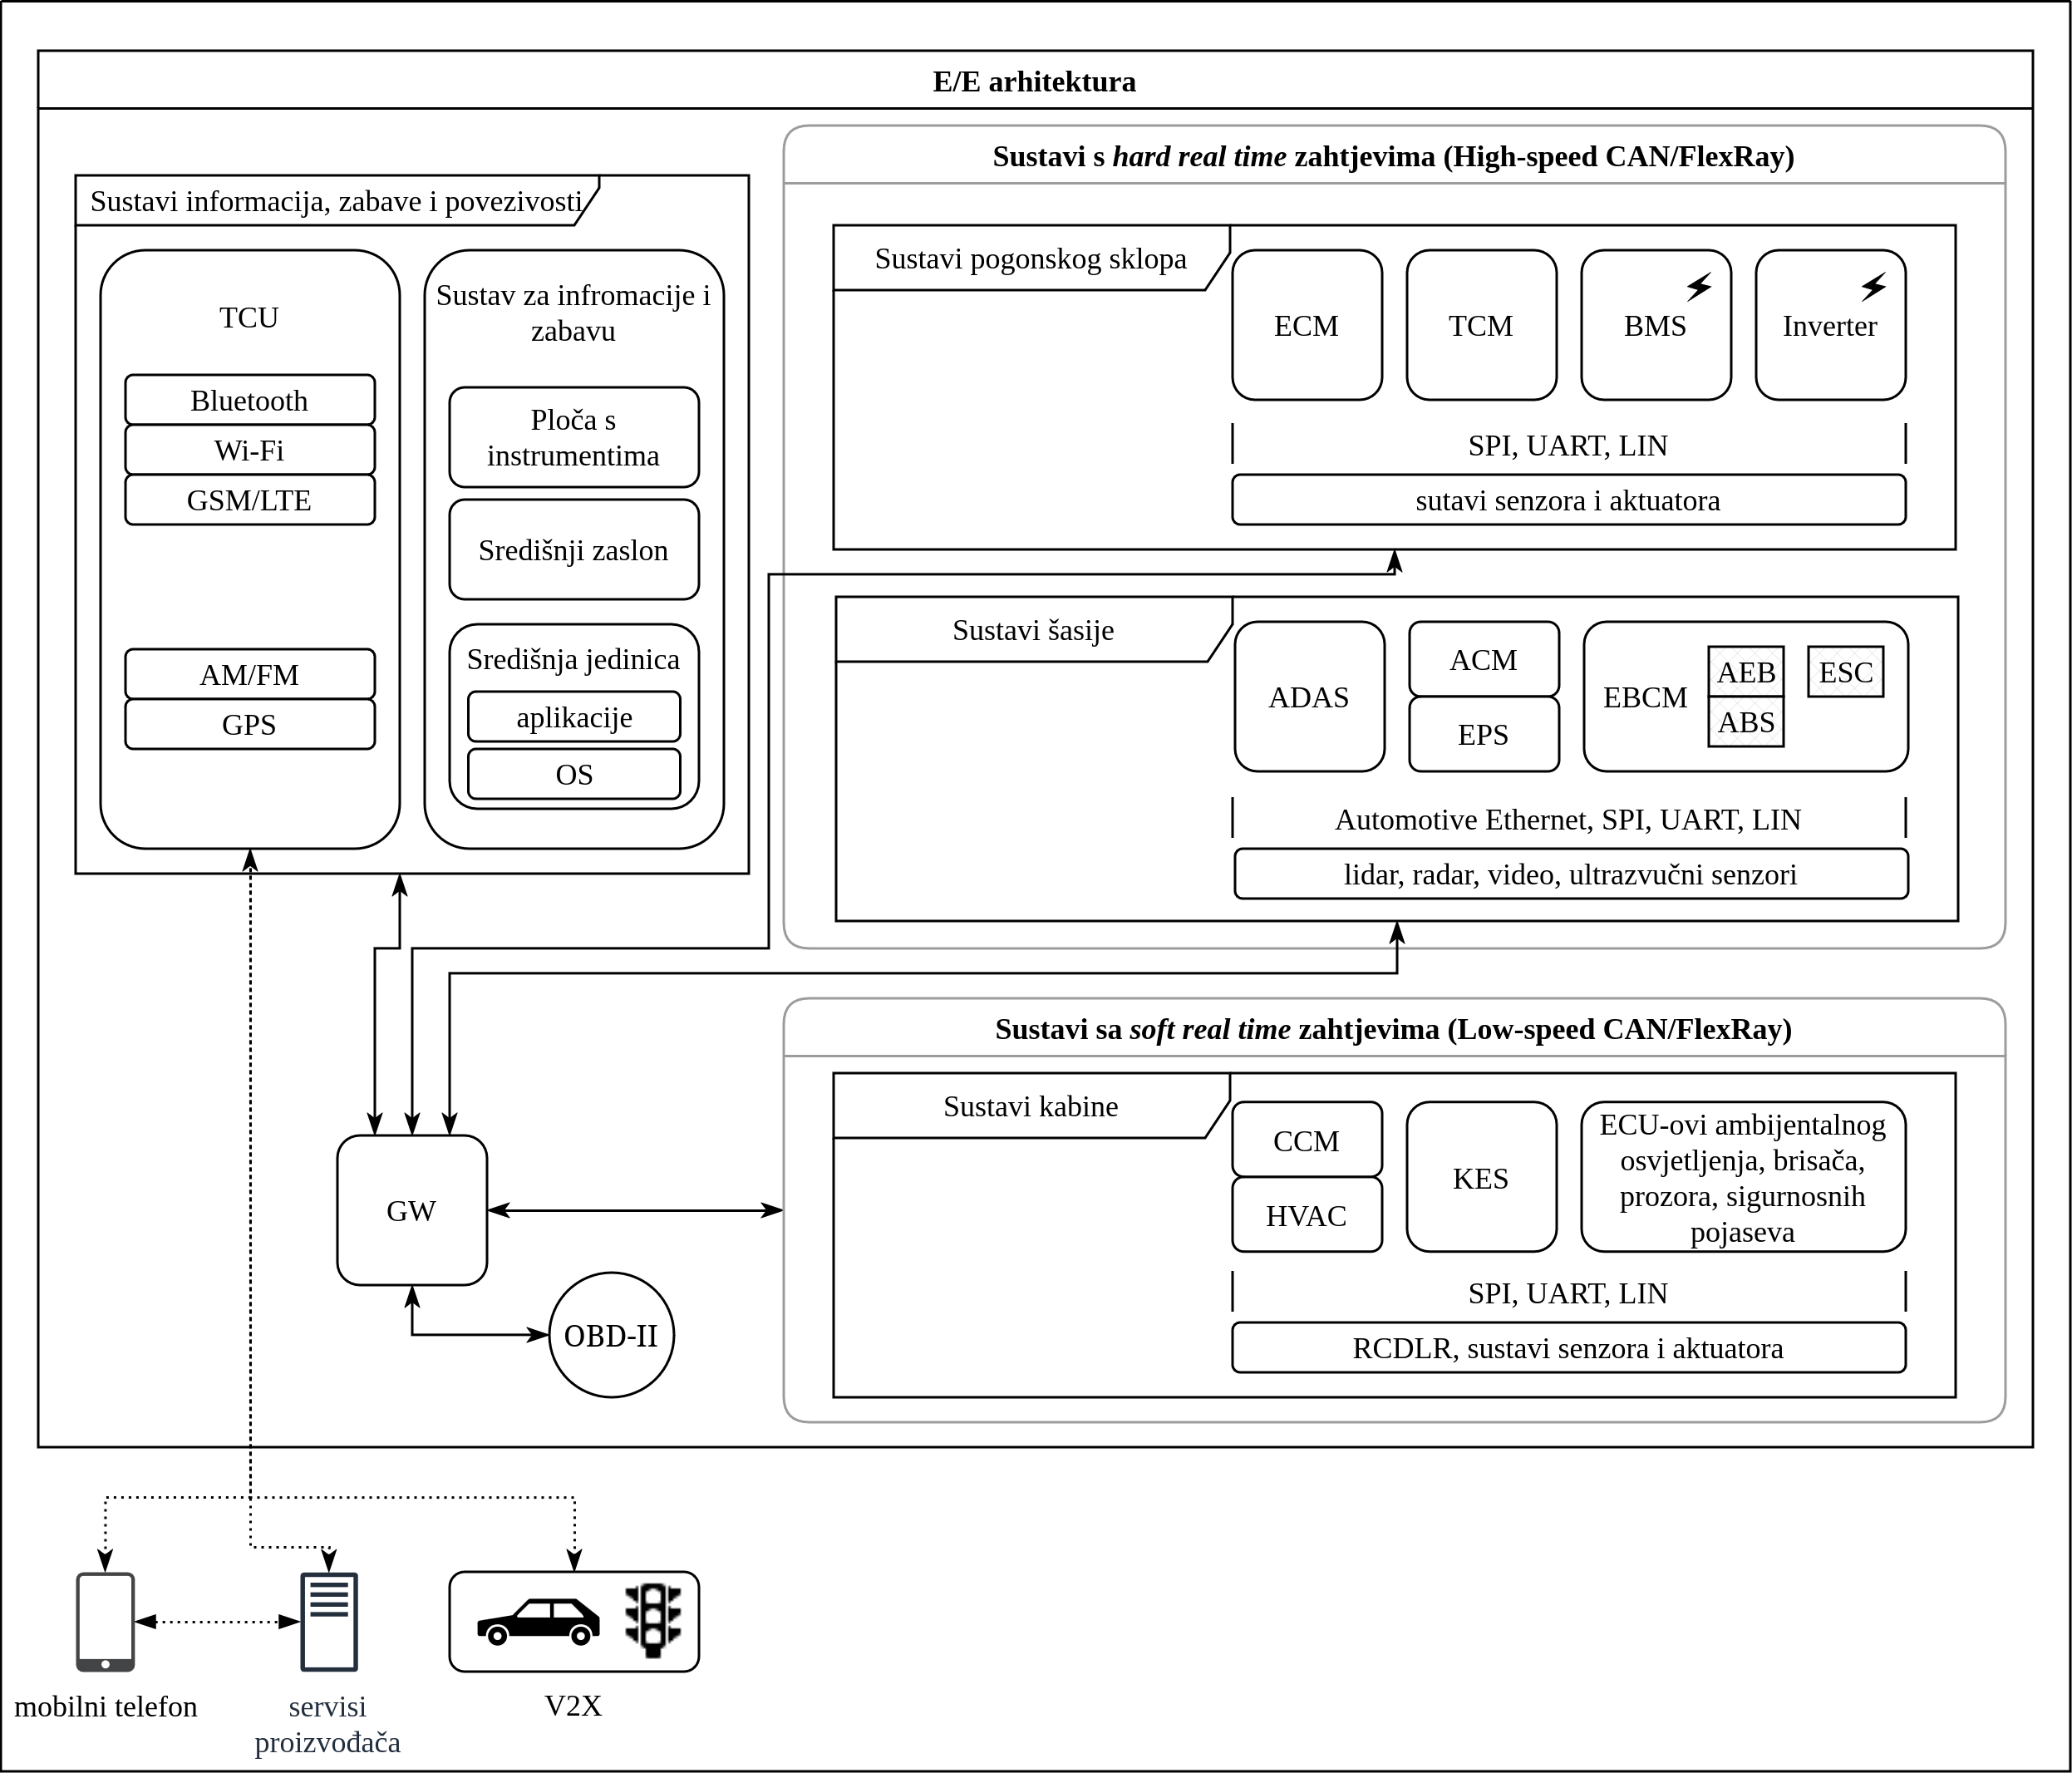
\includegraphics[width=\textwidth]{arhitektura.png}
\caption{Generalizirana arhitektura modernog automobila}
\label{fig:arhitektura}
\end{figure}
\newpage
\section{Protokoli fizičkog sloja i sloja podatkovne poveznice}
\subsection{CAN}
Protokol \textit{Controller area network} je serijski komunikacijski protokol sa svojstvima pogodnima za komunikaciju sustava u stvarnom vremenu\cite{bosch1991}. Predstavili su ga inženjeri tvrtke \textit{Robert Bosch GmbH} 1986. godine, na konferenciji \textit{Society of Automotive Engineers} (SAE) u Detroitu, a prvu primjenu u automobilskoj industriji imao je u modelu \textit{Mercedes-Benz W140}, puštenom na tržište 1991. godine te je danas standard za komunikaciju u motornim vozilima, ali se pojavljuje i u industrijskim upravljačkim sustavima\cite{bosch2022handbook, mercedes1991can}. Specifikacija CAN-a tvrtke \textit{Robert Bosch GmbH} standardizirana je u seriji standarda ISO 11898. 
\newpage
Prema \cite{bosch1991} CAN se može podijeliti u 3 sloja:
\begin{itemize}
    \item objektni sloj \engl{object layer}
    \item prijenosni sloj\engl{transfer layer}
    \item fizički sloj \engl{physical layer}
\end{itemize}
Prema OSI modelu, objektni i prijenosni sloj odgovaraju sloju podatkovne poveznice, a fizički sloj fizičkom. Objektni sloj definira filtriranje primljenih poruka te određivanje poruka koje treba prenijeti. Prijenosni sloj obuhvaća funkcije upravljanja okvirima, arbitraže, signaliziranja i provjeravanja grešaka. Fizički sloj definira kako se zapravo i kojim prijenosnim medijem signali prenose. Glavna svojstva protokola CAN su prioritizacija poruka putem nedestruktivne arbitraže, garancija vremena latencije, mogućnost postojanja više \textit{master} čvorova, detekcija i signalizacija grešaka, razlikovanje privremenih grešaka i trajnih ispada te automatsko isključivanje neispravnih čvorova. 

Na razni fizičkog sloja, razlikujemo CAN visoke brzine \engl{high-speed CAN} i CAN niske brzine \engl{low-speed CAN}, definirani u ISO 11898-2 i ISO 11898-2. CAN visoke brzine može postići brzinu prijenosa podataka do 1 Mbit/s te se koristi za komunikaciju između kritičnijih čvorova, dok je CAN niske brzine tolerantan na greške te ima maksimalnu brzinu prijenosa podataka od 125kbit/s \cite{bosch2022handbook}. Prijenosni medij je parica, koja može biti upredena ili neupredena. Podaci se šalju putem dva komplementarna signala, \textit{CAN Low} (CAN\_L) i \textit{CAN High} (CAN\_H) koji čine diferencijalni par. Razlika između napona signala CAN\_H i CAN\_L definira logičko stanje sabirnice. Diferencijalni signal čini CAN otpornijim na interferenciju, s obzirom na to da će interferencija utjecati na oba signala, ali ne i na njihovu razliku\cite{bosch2022handbook}. 

Nisko logičko stanje odnosno logička \glqq0\grqq je dominantno stanje, a visoko logičko stanje, logička \glqq1\grqq, je recesivno stanje. Logička razina sabirnice u određenom trenutku može se odrediti kao logički umnožak stanja koja na sabirnicu postavljaju čvorovi u tom trenutku. Odnosno, razina sabirnice bit će u dominantnom niskom logičkom stanju u slučaju da barem jedan od čvorova postavlja dominantnu logičku \glqq0\grqq, a u suprotnom biti će u recesivnom stanju, prikazano na primjeru s 3 čvora na slici \ref{fig:sabirnica}. 
\newpage
\begin{figure}[htb]
\centering
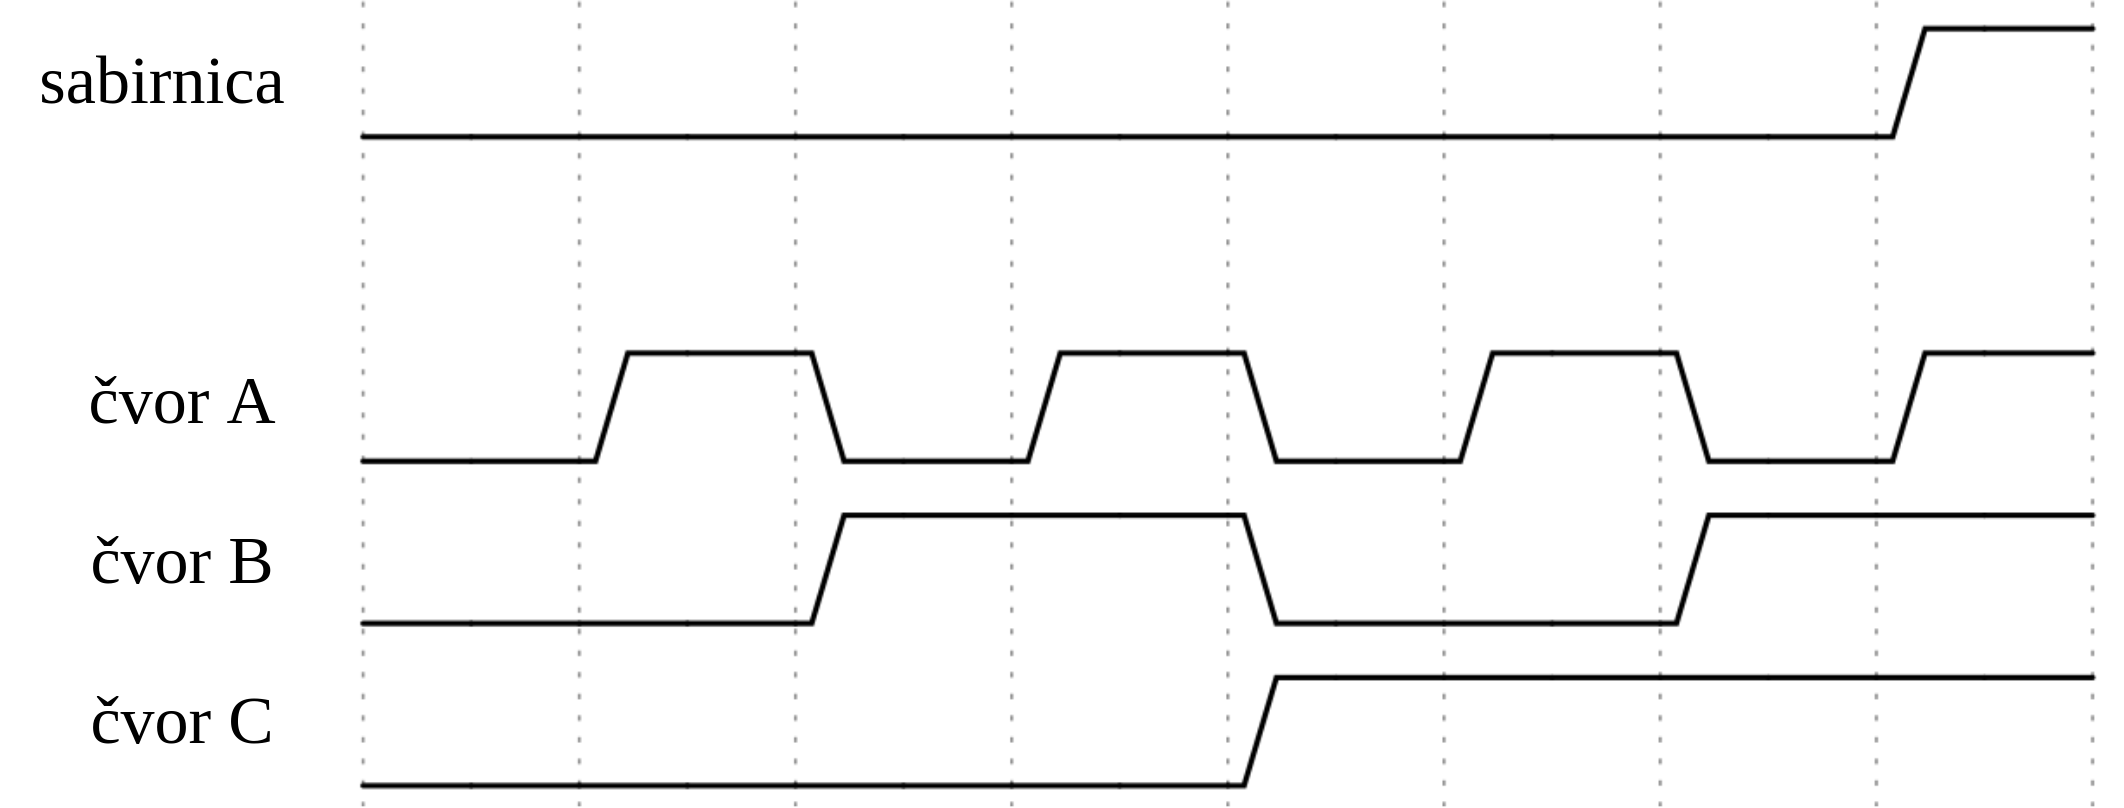
\includegraphics[width=275pt]{slike/sabirnica.png}
\caption{Logička stanja CAN sabirnice}
\label{fig:sabirnica}
\end{figure}

Opisano ponašanje omogućava sustav arbitraže i prioritizacije CAN poruka, kojim se određuje koji čvor ima prednost pri prenošenju podataka u slučaju istovremenog početka prijenosa poruka više čvorova. Svaki CAN okvir započinje bitom za početak okvira (engl. start-of-frame bit, SoF) te arbitražnog identifikatora \engl{arbitration identifier)}. Primjerice, kada dva čvora istovremeno krenu prenositi svoje poruke, odnosno prvo njihove identifikatore, oni će ih prenositi bit po bit sve dok prvi čvor ne zamijeti razliku između postavljenog i stvarnog stanja. Razlika se pojavljuje jer je drugi čvor postavio dominantnu logičku \glqq0\grqq kada je prvi htio postaviti recesivnu logičku \glqq1\grqq. Nakon toga prvi čvor prepušta sabirnicu te se prebacuje u stanje čitanja, a drugi čvor prenosi svoju poruku do kraja. Nakon što sabirnica ponovno postane slobodna, prvi čvor će pokušati napraviti retransmisiju svoje poruke. Sukladno tome, poruke koje imaju manji identifikator, imaju veći prioritet, jer imaju duži neprekinuti niz nula na početku okvira. Primjer s razrješavanjem kolizije između dva čvora dalje se može proširiti na veći broj čvorova, gdje prioritet dobiva čvor čija poruka ima najmanji identifikator, a ostali čekaju završetak prijenosa. Kada se sabirnica ponovno oslobodi, ostali čvorovi započinju retransmisiju te se postupak arbitraže ponavlja.

% opis can okvira
\textit{Boschova} specifikacija inačice 2.0 CAN-a iz 1991. godine dijeli se na dijelove A i B, odnosno CAN 2.0A i CAN2.0B \cite{bosch1991}. Razlikuju se u podržanoj duljini identifikatora poruke, gdje CAN2.0B podržava standardne poruke s 11-bitnim identifikatorima i proširene poruke s 29-bitnim identifikatorima, dok CAN2.0B podržava samo standardne poruke. Razlikujemo 4 vrste CAN okvira:
\begin{itemize}
    \item podatkovni okvir \engl{data frame}
    \item okvir greške \engl{error frame}
    \item okvir zahtjeva \engl{remote frame}
    \item okvir preopterećenja \engl{overload frame}
\end{itemize}
\newpage
Glavni dijelovi podatkovnog okvira prikazanog na slici \ref{fig:CAN_okvir} su:
\begin{enumerate}
    \item bit početka okvira (engl. \textit{Start-of-Frame bit, SOF})    
    \item arbitražni identifikator \engl{arbitration ID}    
    \item bit zahtjeva za prijenosom (engl. \textit{remote transmission request}, RTR) 
    \item bit proširenja identifikatora (engl. \textit{identifier extension bit}, IDE) 
    \item kod duljine podataka {engl. \textit{data length code}, DLC}
    \item podatkovno polje        
    \item kod cikličke provjere zalihosti (engl. cyclic redundancy check)
    \item bit potvrde (\textit{acknowledge slot}, ACK)
    \item kraj okvira (engl. \textit{End-of-Frame}, EOF)        
\end{enumerate}

Uz navedene, na slici \ref{fig:CAN_okvir} pojavljuju se substitucijski bit RTR bita (engl. \textit{substitute remote request}, SSR) i bitovi r0 i r1 rezervirani za moguća proširenja protokola.
Arbitražni identifikator poruke duljine je 11 bita za standardne poruke (CAN 2.0A) i 29 bita za proširene poruke. Poruke s nižom vrijednosti identifikatora imaju veći prioritet pri arbitraži. Skupa s RTR bitom čini arbitražno polje. RTR bit u recesivnoj \glqq1\grqq označava okvir zahtjeva, a u dominantnoj \glqq0\grqq podatkovni okvir. Ovakvim označavanjem okvira postiže se prednost podatkovnog okvira pri arbitraži nad okvirom zahtjeva s istim arbitražnim identifikatorom. Za specificiranje duljine podataka u oktetima koristi se 4-bitno DLC polje od kojih se zapravo koristi 3 bita, s obzirom na to da je duljina podataka ograničena na 8 okteta. Nakon polja s podacima nalaze se CRC kod i ACK bit. Čvor koji prenosi okvir postavlja ACK bit u recesivnu \glqq1\grqq jer očekuje da će bar jedan čvor potvrditi ispravnost poruke postavljanjem stanja sabirnice u dominantnu \glqq0\grqq. Naposljetku se prenosi niz od 7 recesivnih \glqq1\grqq kao oznaka kraja okvira (EOF).

\begin{figure}[htb]
\centering
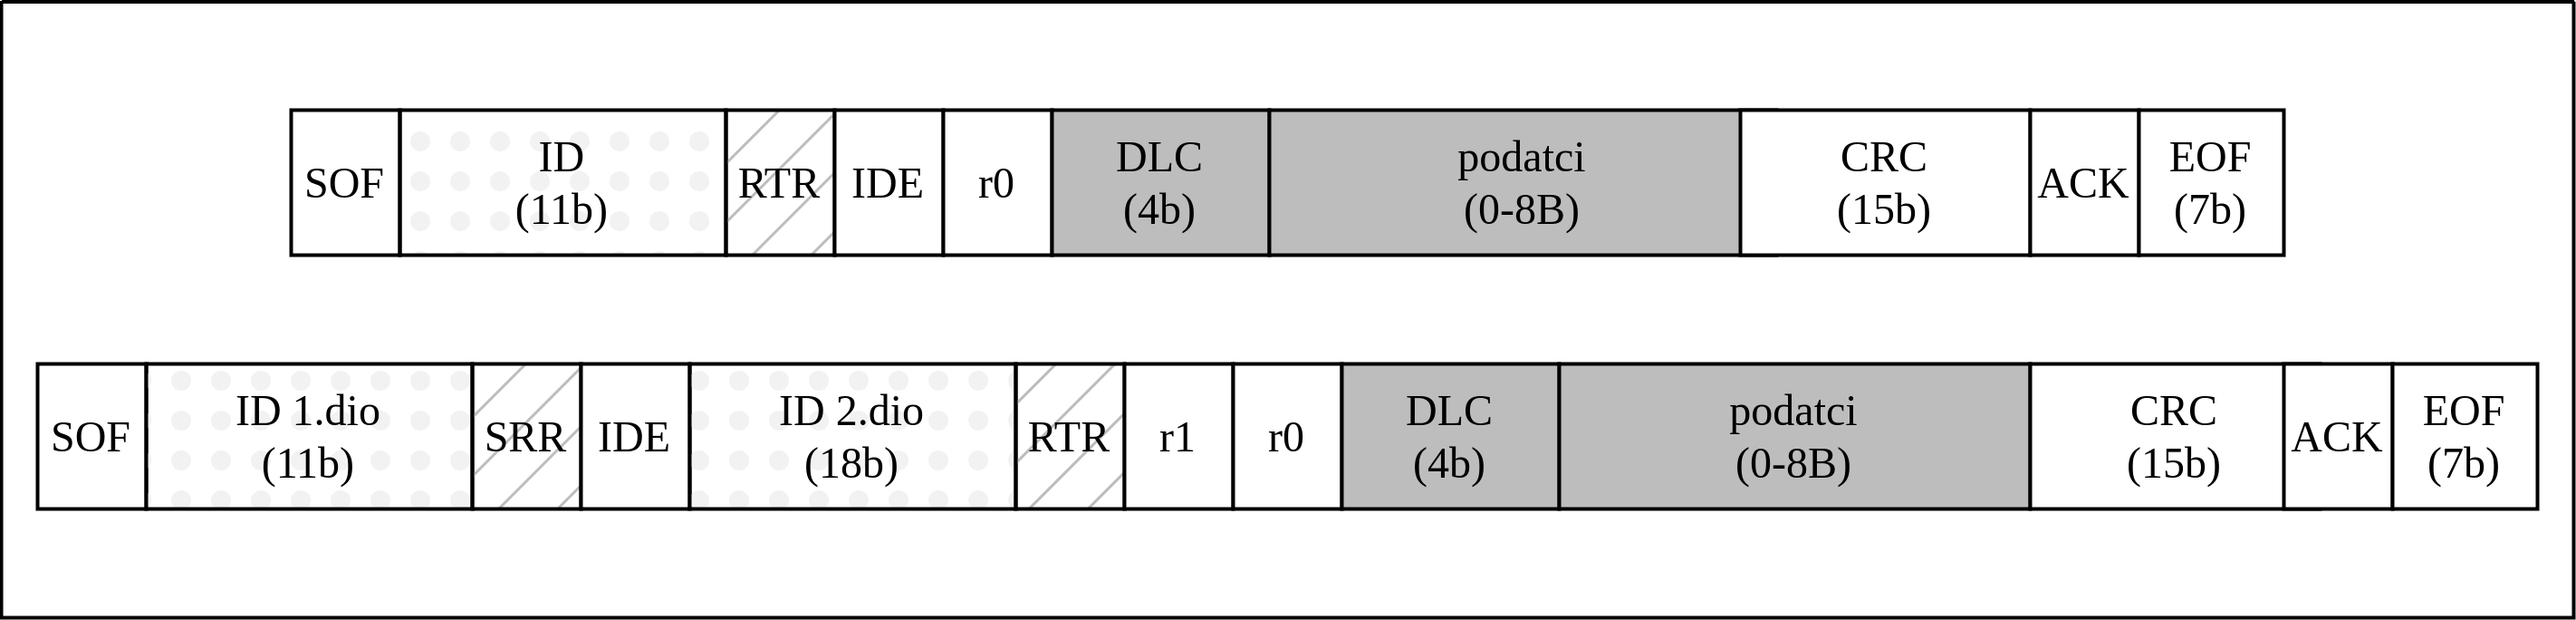
\includegraphics[width=\textwidth]{slike/CAN_okvir.png}
\caption{Standardni i prošireni CAN okvir}
\label{fig:CAN_okvir}
\end{figure}
\newpage
Prema \cite{bosch1991} CAN protokol razlikuje 5 vrsta grešaka:
\begin{itemize}
    \item greška bita \engl{bit error}
    \item greška umetnutog bita \engl{stuff error}
    \item CRC greška \engl{CRC error}
    \item greška formata \engl{form error}
    \item greška potvrde \engl{acknowledgment error}
\end{itemize}

Svaki vrsta greške od navedenih odgovara jednoj od metoda za detekciju grešaka koje su dio CAN protokola. Svaki CAN primopredajnik tijekom prijenosa poruke osluškuje sabirnicu bit po bit kako bi potvrdio da se njegova poruka ispravno prenosi. Ako se postavljeni bit i stvarni bit na sabirnici razlikuju, osim u periodu arbitraže, CAN primopredajnik će detektirati grešku bita. CAN protokol koristi i \textit{bit stuffing} metodu detekcije grešaka, odnosno umetanje dodatnog bita suprotnog polariteta nakon 5 bitova istog polariteta. Dodatne bitove uklanja primopredajnik čvora primatelja. Greškom umetnutog bita smatra se pojavljivanje 6 bita istog polariteta. Svaki čvor primatelj izračunava CRC kod primljene poruke, a razlika u izračunatom i primljenom CRC kodu smatra se CRC greškom. CAN okviri sadrže nekoliko fiksnih bitova, čija neispravnost naznačava grešku formata. Naposljetku, grešku potvrde detektira čvor pošiljatelj kada niti jedan čvor primatelj nije postavio sabirnicu u dominantnu \glqq0\grqq tijekom perioda ACK bita.

Svaki čvor interno održava dva brojača grešaka, brojač grešaka pri prijenosu (engl. \textit{transmit error counter}, TEC) te brojač grešaka pri primitku (engl. \textit{receive error counter}, REC). Brojači se koriste u sklopu CAN-ovog mehanizma lokalizacije grešaka (engl. \engl{error confinment mechanism} U kontekstu grešaka, čvorovi mogu biti u aktivnom, pasivnom i stanju ispada \engl{bus off}. Trenutno stanje čvora ovisi o vrijednostima TEC i REC brojača, prikazano konačnim automatom stanja na slici \ref{fig:error_stanja}. Kada čvor u aktivnom stanju detektira grešku postavlja aktivnu zastavicu greške u obliku 6 dominatnih bitova koji će sigurno trenutni okvir učiniti nevažećim zbog metode \textit{bit stuffing} te će ostali čvorovi u aktivnom stanju analogno reagirati postavljanjem svojih zastavica. Ovisno na kojem od 6 bitova prve zastavice ostali čvorovi detektiraju grešku, duljina cjelokupnog okvira greške može biti između 6 i 12 bitova. Čvor u pasivnom stanju u slučaju detektiranja greške postavlja pasivnu zastavicu greške u obliku 6 recesivnih bitova, u svrhu samoprovjere čvora, što može rezultirati u promjeni stanja brojača. 
\newpage
\begin{figure}[htb]
\centering
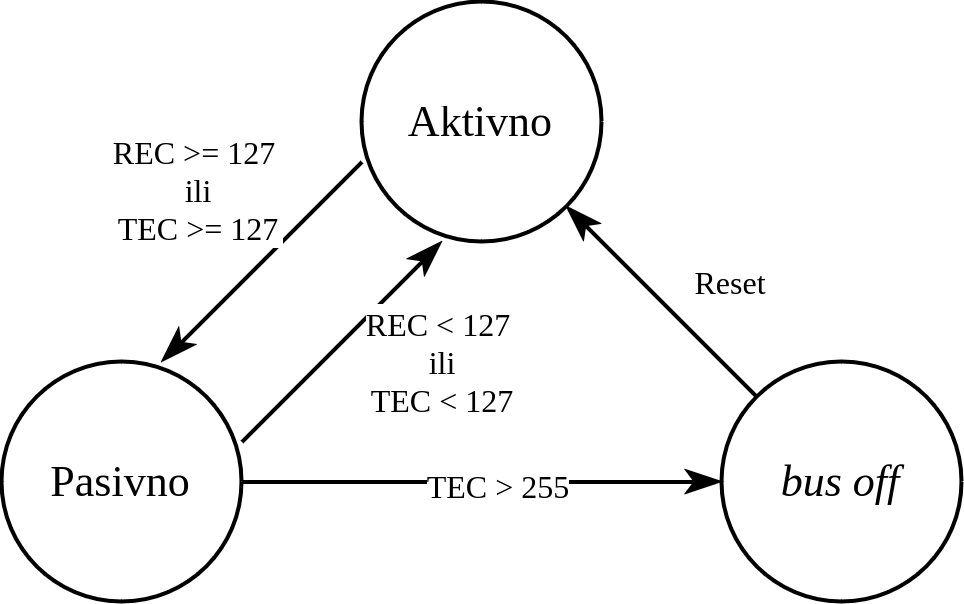
\includegraphics[width=230pt]{slike/stanja.png}
\caption{Stanja CAN čvora}
\label{fig:error_stanja}
\end{figure}

S obzirom na to da je maksimalna brzina prijenosa podataka klasičnog CAN-a 1 Mbit/s s ograničenjem od maksimalno 8 okteta podataka po poruci, tvrtka \textit{Robert Bosch GmbH} uvodi CAN s fleksibilnom brzinom prijenosa podataka (engl. \textit{CAN with Flexible Data-Rate}, CAN-FD) kao proširenje CAN-a. CAN-FD povećava maksimalnu duljinu polja podataka jednog okvira s 8 na 64 okteta. Uz navedeno, omogućava dinamično povećanje brzine prijenosa, uobičajeno do 2Mbit/s, isključivo za vrijeme trajanja prijenosa podataka nekog CAN okvira \cite{bosch2022handbook,nasser2023automotive}.

\subsection{FlexRay}
Zbog potrebe za više determinističkim komunikacijskim protokolom s garantiranom propusnosti za kritične poruke, stvoren je FlexRay \cite{nasser2023automotive}. FlexRay za razliku od CAN-a, koji koristi \textit{Code Division Multiple Access} metodu dodjeljivanja pristupa sabirnici, FlexRay koristi \textit{Time Division Multiple Access} metodu koja dodjeljuje pristup za prijenos određenih poruka po vremenskim odsječcima u dva kanala. Poruke mogu biti periodične, fiksne duljine te se za njih dodjeljuju statički vremenski odsječci ili su neperiodične, varijabilne duljine te se onda prenose u dinamičkom vremenskom odsječku \cite{nasser2023automotive}. Maksimalna duljina polja podataka jedne poruke je 254 okteta, što omogućava brzinu prijenosa podataka do 10Mbit/s u slučaju konfiguracije s jednim redundantnim kanalom. Ukoliko komunikacija nije kritična, redundantni kanal moguće je iskoristiti za udvostručenje brzine prijenosa podataka do 20Mbit/s \cite{nasser2023automotive, bosch2022handbook}. FlexRay mreže mogu biti organizirane u sabirničku topologiju ili topologiju zvijezde.
\subsection{Ethernet}
Pojava sustava s potrebama za još većom brzinom prijenosa podataka, potaknula je proizvođače na uporabu Etherneta prilagođenog za primjenu u automobilskoj industriji \engl{automotive Ethernet} u internim mrežama svojih vozila \cite{nasser2023automotive, bosch2022handbook}. Brzine prijenosa podataka kreću se u rasponu od 10Mbit/s do 10Gbit/s, što Ethernet čini priladnim za vremenski osjetljivu komunikaciju, poput spajanja domenskih upravljačkih jedinica te za primjene koje zahtjevaju veliku propusnost, primjerice prijenos video toka između ADAS-a i video senzora. Ethernet također nema sigurnosne probleme koje donosi CAN zbog kompatibilnosti s postojećim tehnologijama poput IPsec-a, MACsec-a te TLS-a \cite{vector2021uds}.

Najveća prilagodbe za automobilsku industriju pojavljuju se na fizičkom sloju, koji mora biti prilagođen standardima elektromagnetske kompatibilnosti (engl. \textit{electromagnetic compatibility}, EMC).
\subsection{LIN}
\textit{Local Interconnect Network} sabirnica najčešću primjernu ima u povezivanju senzora i aktuatora s pripadajućim ECU-ovima . Primjerice, koristi se u sustavima domene šasije za upravljanje bravom vrata, podizanjem i spuštanjem prozora te namještanjem zrcala retrovizora \cite{bosch2022handbook, nasser2023automotive, dissecto2023networks}. U automobilima LIN komunikacija odvija se između \textit{master} ECU-a, koji zadaje naredbe i \textit{slave} senzora i aktuatora koji ih obrađuju i po potrebi odgovaraju. Komunikaciju pokreće \textit{master} prijenosom zaglavlja koje sadrži sinkronizacijske bitove te identifikator naredbe. \textit{Slave} odgovara prijenosom podataka maksimalne duljine 8 okteta i kontrolne sume. Iako je sporiji od CAN-a s brzinom prijenosa podataka do 20kbit/s te podržava manje fleksibilnu konfiguraciju od maksimalno 16 čvorova, prednost LIN-a je jeftin prijenosni medij u obliku jednožilnog kabela.
\section{Dijagnostički i kalibracijski protokoli}
 Dijagnostički i kalibracijski protokoli su protokoli aplikacijskog sloja OSI modela te mogu funkcionirati povrh različitih protokola nižih slojeva, ali su u ovom radu razmatrani u kontekstu CAN-a. U ovom poglavlju opisani su dijagnostički protokoli \textit{Unified Diagnostic Services} (UDS) i \textit{On Board Diagnostics II} (OBD-II) te univerzalni mjerni i kalibracijski protokol (engl. \textit{Universal Measurement and Calibration Protocol}, XCP). 
 
\subsection{Transportni protokol ISO-15765-2}
Preduvjet za ispravnu komunikaciju putem protokola UDS i OBD-II je povećanje maksimalne duljine prenesenih podataka u jednom CAN okviru. U tu svrhu, kroz standard ISO 15765, uveden je ISO-15765 transportni protokol (ISO-TP) koji omogućava pouzdan prijenos podataka veličine do 4GB povrh CAN-a ili CAN-FD-a \cite{dissecto2023isotp}. ISO-TP uvodi 6 načina adresiranja čvorova, gdje se pri korištenju normalnog načina adresiranja svakom čvoru pridjeljuju dva arbitražna identifikatora, za primanje i slanje poruka.

Podaci veći od maksimalne veličine polja podataka CAN ili CAN-FD okvira, fragmentiraju se u jedan \textit{First Frame} (FF) okvir te u više uzastopnih \textit{Consecutive Frame} (CF) okvira. Nakon FF okvira te prije primitka ostatka podataka kroz više CF okvira, primatelj mora prvo poslati \textit{Flow Control} okvir, kojim definira parametre veličine bloka i vremenskog razmaka. U slučaju da su podaci manji od maksimalne veličine polja podataka CAN ili CAN-FD okvira, prenose se \textit{Single Frame} okvirom.  

\subsection{OBD-II}
Zahtjev za uvođenjem dijagnostike u svrhu kontrole emisija u svim novim automobilima izdao je \textit{California Air Resources Board} u Kaliforniji 1991. godine. Navedena dijagnostika je nazvana \textit{On Board Diagnostics} (OBD) te je 1994. standardizirana pod nazivom OBD-II. OBD-II definira standardizirani skup dijagnostičkih informacija koje svaki ECU mora čuvati te priključak i komunikacijski protokol za pristup navedenom skupu \cite{bosch2022handbook}.

Od 2014. godine u Europskoj Uniji dozovoljeno je samo korištenje CAN-a na fizičkom sloju i sloju podatkovne poveznice te protokola ISO-TP na transportnom sloju, što je u skladu sa standardom ISO 15767 \cite{bosch2022handbook}. Međutim, priključak OBD-II uz CAN podržava i protokole \textit{Keyword Protocol 2000}, VPW i PWM te protokol standarda ISO 9141-2. Shema priključka OBD-II s označenim CAN kontaktima prikazana je na slici \ref{fig:obd2} \cite{falch2022obd}.

\begin{figure}[htb]
\centering
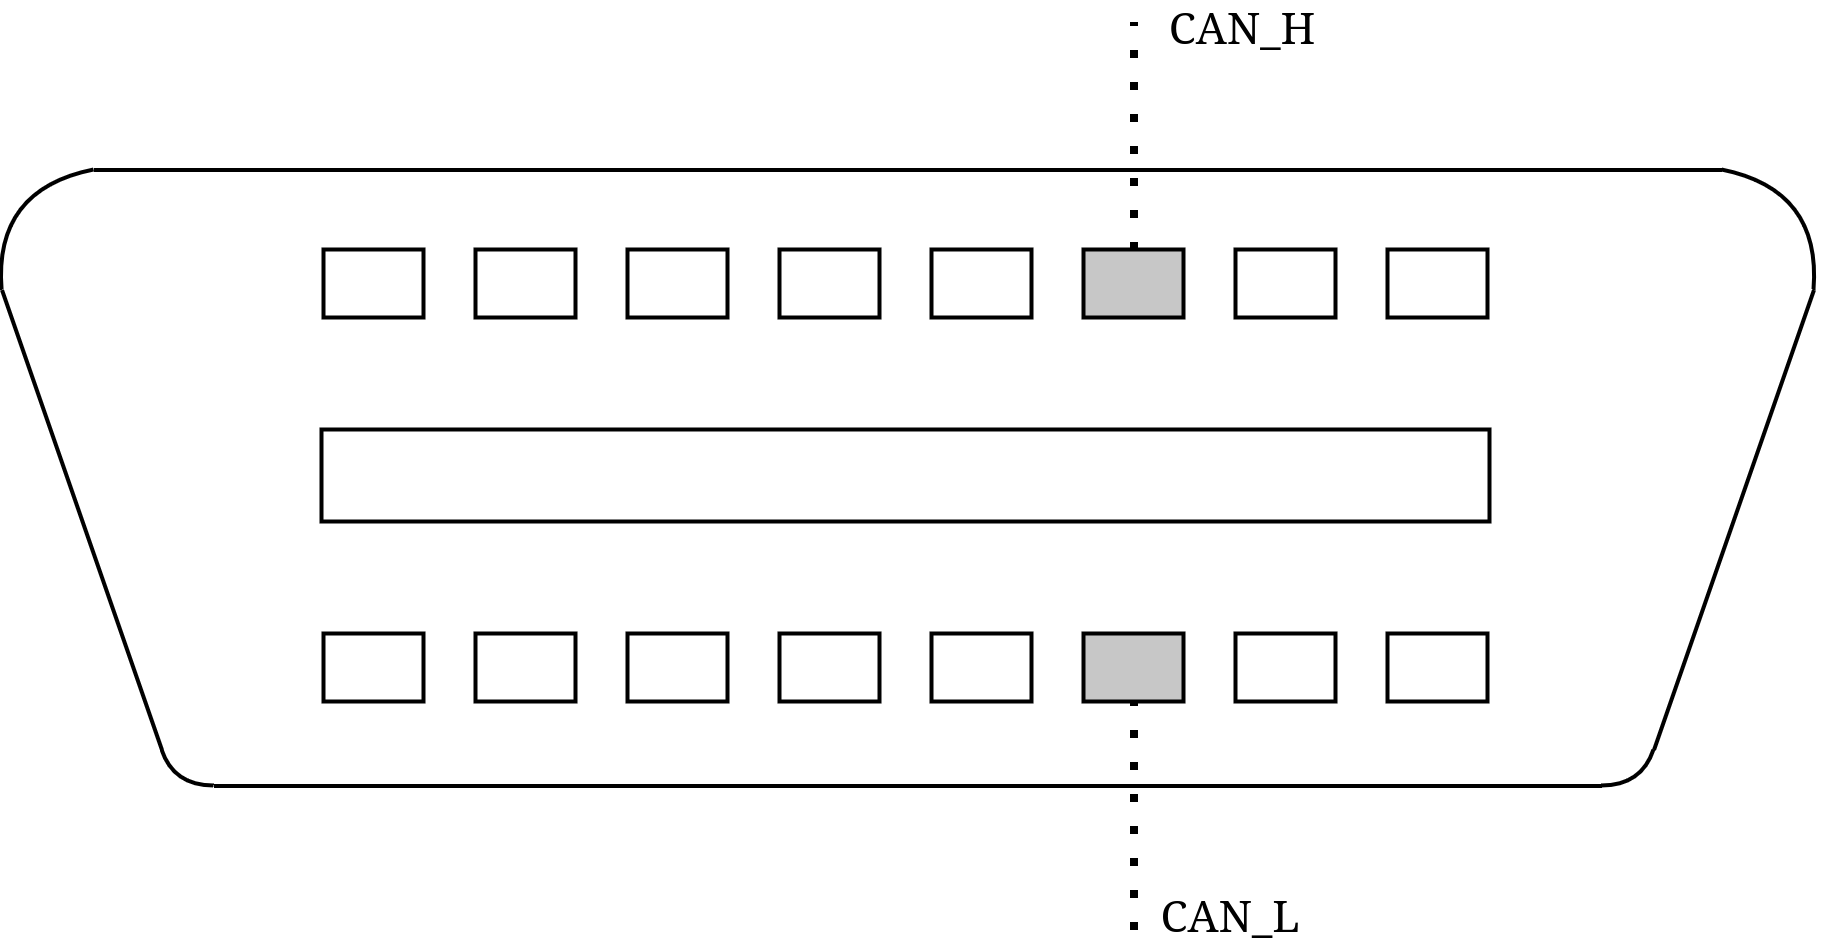
\includegraphics[width=250pt]{slike/obd2.png}
\caption{Shema OBD-II priključka}
\label{fig:obd2}
\end{figure}

Zahtjevi u protokolu OBD-II šalju se s arbitražnim identifikatorom \texttt{0x7DF}, a odgovori na zahtjeve s identifikatorima \texttt{0x7E8} do \texttt{0x7EF}. Dijagnostičke informacije poput trenutne brzine, broja okretaja te temperature motora, moguće je dohvatiti korištenjem različitih servisa s njihovim paramtarskim identifikatorima (engl. \textit{Parameter identificator}, PID). Specifičan je servis \texttt{03}, koji nudi isčitavanje dijagnostičkih kodova neispravnosti (engl. \textit{diagnostic trouble code}, DTC) te servis \texttt{04} koji omogućava njihovo brisanje \cite{falch2022xcp}.

\subsection{UDS}
\textit{Unified Diagnostic Services} (UDS) je protokol aplikacijskog sloja koji nudi niz dijagnostičkih servisa koje je moguće implementirati za pojedini ECU. Standardiziran je u ISO 14229 te povrh CAN-a koristi ISO-TP na transportnom sloju \cite{dissecto2023uds}.

ECU se u UDS komunikaciji ponaša kao poslužitelj, dok je klijent najčešće dijagnostički alat servisera ili programska podrška za konfiguraciju ECU-ova u tvornici. Kroz niz UDS servisa moguće je upravljati stanjem ili ponovno pokrenuti ECU, čitati i brisati DTC-ove, isčitavati i modificirati parametre ECU-a, testirati značajke ECU-a korištenjem ugrađenih rutina te isčitavati i modificirati sadržaj memorije, prvenstveno u svrhu ažuriranja \cite{falch2022uds}. UDS zahtjev sastoji se od identifikatora servisa (engl. \textit{service identifier}, SID), okteta podfunkcije odabranog servisa, skupa s potrebnim parametrima, prikazano na slici \ref{fig:uds}. Ukoliko je odgovor pozitivan, sadržavat će SID uvećan za 0x40 te podatke odgovora specifične tom servisu. U slučaju negativnog odogvora, odgovor počinje s oketom \texttt{0x7F} te sadrži SID zahtjevanog servisa te kod negativnog odgovora (engl. \textit{negative response code}, NRC), primjerice kod \texttt{0x11} u slučaju da ECU ne podržava zahtjevani servis. 

\bigskip
\begin{figure}[htb]
\centering
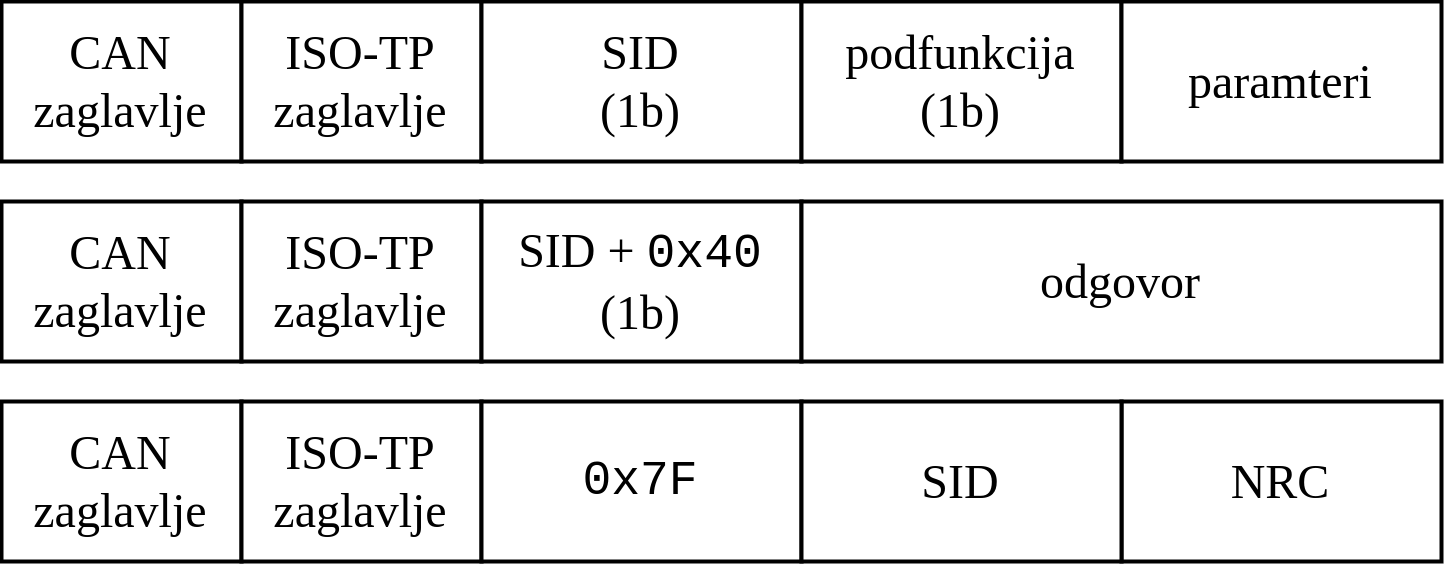
\includegraphics[width=300pt]{slike/uds.png}
\caption{UDS zahtjev, pozitivan i negativan odgovor}
\label{fig:uds}
\end{figure}

\newpage
Između 27 dostupnih UDS servisa, kao sigurnosno kritične UDS servise treba izdvojiti:
\begin{itemize}
    \item \texttt{0x10 DiagnosticSessionControl}
    \item \texttt{0x11 ECUReset}
    \item \texttt{0x28 CommunicationControl}
    \bigskip
    \item \texttt{0x22 ReadDataByIdentifier}
    \item \texttt{0x23 ReadMemoryByAddress}
    \item \texttt{0x2E WriteDataByIdentifier}
    \item \texttt{0x3D WriteMemoryByAddress}
    \bigskip
    \item \texttt{0x34 RequestDownload}
    \item \texttt{0x35 RequestUpload}
    \item \texttt{0x38 RequestFileTransfer}
    \bigskip
    \item \texttt{0x2F InputOutputControlByIdentifier}
    \item \texttt{0x31 RoutineControl}
    \bigskip
    \item \texttt{0x27 SecurityAccess}
    \item \texttt{0x29 Authentication}
\end{itemize}

Servis \texttt{DiagnosticSessionControl} koristi se za izmjenu vrste dijagnostičke sesije. Dijagnostička sesija određuje kontekst izvršavanja servisa, primjerice kojem dijelu memorije se pristupa i koji dio izvršnog koda se može ažurirati. Također, servisi mogu biti podijeljeni po različitim vrstama dijagnostičkih sesija, čime se omogućava ili onemogućava njihovo korištenje. Servis \texttt{ECUReset} koristi se za pokretanje više različitih vrsta resetova ECU-ova. Vrstu reseta određuje oktet podfunkcije. Zabrana primanja i slanja poruka nekom ECU-u može se uvesti korištenjem servisa \texttt{CommunicationControl}.

Servisi \texttt{ReadDataByIdentifier} i \texttt{WriteDataByIdentifier} koriste se u svrhu čitanja i pisanja podataka spremljenima pod određenim podatkovnim identifikatorima (engl. \textit{data identifier}, DID). Značenje većine identifikatora određuje proizvođač. Za čitanje i pisanje u memoriju ECU-a koriste se servisi \texttt{ReadMemoryByAddress} i \texttt{WriteMemoryByAddress}, gdje dostupnost dijelova memorije ovisi o konkretnoj implementaciji\cite{falch2022uds, dissecto2023uds}.

Skupini servisa \texttt{0x34} do \texttt{0x38} koji služe za preuzimanje i prijenos podataka pripadaju servisi \texttt{RequestUpload}, texttt{RequestDownload} te \texttt{RequestFileTransfer}. Servisi \texttt{RequestUpload} i \texttt{RequestDownload} koriste se za započinjanje prijenosa izvršnog koda s testirane jedinice prema klijentu te obrnuto. Servis \texttt{RequestFileTransfer} koristi se za preuzimanje ili prijenos datoteka te dohvaćanje informacija o datotečnom sustavu ECU-a. Navedeni servisi često služe za distribuciju OTA ažuriranja pojedinim ECU-ovima nakon što je ažuriranje preuzeto putem mobilne ili Wi-Fi mreže.

Servis \texttt{InputOutputControlByIdentifier} omogućava klijentu upravljanje signalima koje ECU odašilje, njihovo zamrzavanje na trenutnoj vrijednosti ili resetiranje na pretpostavljenu vrijednost. Servis \textit{RoutineControl} omogućava klijentu aktivaciju i deaktivaciju pretprogramiranih testnih rutina te dohvaćanje njihovih rezultata.

Naposljetku, za sve UDS servise moguće je omogućiti autorizaciju ili autentifikaciju s više razina pristupa putem servisa \texttt{SecurityAccess} ili \texttt{Authentication}. Servis \texttt{0x27 SecurityAccess} koristi nespecificirani \textit{seed-and-key} algoritam. Pojam \textit{seed-and-key} upotrebljava se u UDS specifikaciji umjesto pojma izazov-odgovor \engl{challenge-response} koji je čest u ostalim granama kibernetičke sigurnosti. Slijed autorizacije servisom \texttt{0x27} može se prikazati kroz nekoliko koraka:
\begin{enumerate}
    \item Klijent šalje zahtjev za autorizacijom te dodatne parametre poput zahtjevane razine pristupa.
    \item ECU generira niz okteta \textit{seed} i šalje ga klijentu.
    \item Klijent i ECU koriste \textit{seed} kao ulaz u \textit{seed-and-key} algoritam te izračunavaju ključ.
    \item Klijent šalje \textit{seed} ECU-u.
    \item ECU uspoređuje primljeni ključ s izračunatim te odobrava ili odbija pristup klijentu.
\end{enumerate}
Sigurnost autorizacije putem servisa \texttt{SecurityAccess} ovisi o odabranom \textit{seed-and-key} algoritmu.
Servis \texttt{Authentication} dodan je u reviziji standarda ISO-14229-1:2020 kao moderna alternativa servisu \texttt{SecurityAccess}. Temelji se na korištenju digitalnih certifikata i infrastrukture javnog ključa (engl. \textit{public key infrastructure, PKI} za autentifikaciju \cite{vector2021uds}:
\begin{enumerate}
    \item Klijent šalje zahtjev za autentifikacijom te svoj digitalni certifikat s javnim ključem.
    \item ECU verificira certifikat provjeravajući njegov potpis s javnim ključem certifikacijskog autortiteta kojem vjeruje.
    \item ECU generira niz okteta \textit{challenge} i šalje ga klijentu.
    \item Klijent izračunava digitalni potpis koristeći \textit{challenge} te svoj privatni ključ te ga šalje ECU-u.
    \item ECU verificira ispravnost potpisa koristeći javni ključ klijenta te odobrava ili odbija pristup klijentu.
\end{enumerate}

\subsection{XCP}
Protokol XCP proširenje je CAN kalibracijskog protokola (engl. \textit{CAN Calibration Protocol}, CCP) s podrškom za Ethernet, SPI, USB, FlexRay i CAN-FD kao nižim slojevima umjesto klasičnog CAN-a \cite{falch2022xcp}. Koristi se za mjerenje i kalibraciju parametara i programiranje flash memorije ECU-ova. Najčešće se koristi samo za vrijeme razvoja i testiranja ECU-a \cite{falch2022xcp}.

Komunikacija je oblika \textit{master-slave}, gdje je kalibracijski alat \textit{master}, a ECU \textit{slave}. \textit{Master} s ECU-om komunicira putem zahtjeva nazvanih \textit{Command Receive Object} (CRO) te od ECU-a dobiva \textit{Data Transmission Object} (DTO) odgovore. DTO može biti poruka odgovora na naredbu (engl. \textit{Command Response Message}, CRM), poruka događaja (engl. \textit{Event Message}, EV) te poruka dohvaćanja podataka (engl. \textit{Data Acquisition Message}, DAQ).

U slučajevima kada XCP treba ostati dostupan i nakon prodaje, moguće je kontrolirati pristup korištenjem \textit{seed-and-key} autorizacije. Za autorizaciju se koriste CRO-ovi \texttt{GET\_SEED} i \texttt{UNLOCK}, a koraci autorizacije isti su kao i kod UDS servisa \texttt{Security Access}.
\chapter{Ranjivosti i napadi na protokole i sustave automobila}

Pri izradi CTF zadataka s ciljem edukacije stručnjaka u određenom području, potrebno je razmotriti stvarne napade, incidente, tehnike i otkrivene ranjivosti kako bi se utvrdili najčešći vektori napada te potencijalno ranjive površine napada. Implementiranjem zadataka u skladu s navedenim razmatranjima, zadaci će biti bliži konfiguracijama sustava s kojima se budući stručnjak može susresti u praksi.

U nastavku su najviše razmatrani napadi i ranjivosti iz postojećih sigurnosnih istraživanja jer najdetaljnije prikazuju tehničku razinu koju je potrebno simulirati CTF zadacima.

\section{Ranjivosti i napadi na protokole automobila}
Prethodno razmatranju napada na sustave automobila, potrebno je razumjeti inherentne ranjivosti protokola kojima oni komuniciraju. Ranjivosti ovih protokola proizlaze iz njihove specifikacije, u kojima sigurnosne mjere nisu uopće razmatrane ili nisu u potpunosti definirane.
\subsection{CAN}
U specifikaciji inačice 2.0 protokola CAN, definiran je kao \glqq serijski komunikacijski protokol koji efikasno podržava raspodijeljeno \textit{realtime} upravljanje s visokom razinom sigurnosti\grqq \cite{bosch1991}. Raširenost njegove upotrebe u \textit{realtime} sustavima potvrđuje prvi dio navedene definicije. Međutim, po pitanju sigurnosti specifikacija ne spominje nikakve mjere. Bozdal et al. ističu u \cite{bozdal2020evaluation} da protkol CAN ne osigurava niti jedno od svojstava povjerljivosti, integriteta i dostupnosti. CAN komunikacija je po prirodi \textit{broadcast} odnosno svi čvorovi na sabirnici mogu čitati sve poruke. CAN specifikacija ne definira mehanizam njihovog šifriranja, čime se narušava svojstvo povjerljivosti. Uz svaku CAN poruku šalje se i njen CRC u svrhu provjere njenog integriteta odnosno detekcije grešaka. Međutim, napadaču koji je presreo CAN poruku trivijalno je ponovno izračunati CRC u slučaju da ju želi modificirati, čime se svojstvo integriteta narušava. Svojstvo dostupnosti se također može trivijalno narušiti korištenjem mehanizma CAN-ovog prioritiziranja poruka ili drugim napadima opisanima u nastavku.

Najjednostavniji napad uskraćivanja usluge (engl. \textit{denial of service}, DoS) je napad preplavljivanja sabirnice \engl{bus flood attack} koji iskorištava mehanizam prioritiziranja poruka s nižom vrijednosti arbitražnog identifikatora \cite{tindell2022can}. Napadač s pristupom sabirnici, izravno, putem OBD-II priključka ili kompromitiranog ECU-a, može ju preplaviti porukama s identifikatorom \glqq0\grqq. Ukoliko dodatne mjere nisu implementirane, takve poruke uvijek dobivaju prioritet u postupku arbitraže sabirnice te onemogućavaju komunikaciju ostalih uređaja na sabirnici.

\textit{Bus off} napad je također napad uskraćivanja usluge, koji iskorištava CAN-ov mehanizam lokalizacije grešaka \cite{cho2016error}. Napadač s pristupom sabirnici može bilo koji ECU prebaciti u \textit{bus off} stanje postavljanjem dominantnih bitova na sabirnicu dok ciljani ECU prenosi svoje poruke. Ovim postupkom, ECU će akumulirati velik broj grešaka pri prijenosu i povećati TEC na vrijednost veću od 255, nakon čega ECU prelazi u \textit{bus off} stanje i prestaje emitirati poruke dok se ne oporavi.

Tindell u \cite{tindell2022can} predstavlja novi napad uskraćivanja usluge nazvan \textit{freeze doom loop} koji iskorištava sustav signalizacije preopterećenja sabirnice. U protokolu CAN, definiran je niz bitova koji mora proći između svakog podatkovnog okvira te se naziva \textit{inter-frame space} (IFS). Postavljanje prvog od tih bitova u dominantnu \glqq0\grqq, pojedini ECU može signalizirati svoje preopterećenje. Nakon signalizacije, svi ECU-ovi na sabirnici ulaze u postupak oporavka od greške te prestaju prenositi podatkovne okvire. Napadač može periodički signalizirati preopterećenje nakon svakog perioda oporavka te efektivno zamrznuti sabirnicu na proizvoljno vrijeme. Uz navedeno, signalizacija preopterećenja ne inkrementira brojače grešaka, što može biti potencijalno korisno svojstvo.

Protokol CAN je podložan i napadima lažiranjem poruka \engl{spoofing}. S obzirom na to da u protokol nije ugrađena provjera autentičnosti poruka, napadač može bilo koju poruku postaviti na sabirnicu, lažno se predstavljajući kao čvor koji ju inače prenosi. Primjerice, ako napadač dokuči format poruke za pokretanje motora, ne postoji mehanizam koji ga sprječava da ju pošalje ECM-u umjesto imobilizatora te neovlašteno pokrene motor. 

Ukoliko napadač želi osigurati da komunikacija za vrijeme \textit{spoofing} napada na sabirnici izgleda legitimno, time potencijalno izbjegavajući sustave za otkrivanje napada (engl. \textit{intrusion detection system}, IDS), napadač može prvo natjerati ciljani čvor u \textit{error passive} stanje uništavanjem njegovih poruka postavljanjem dominantnog bita na sabirnicu za vrijeme njihovog prijenosa. U \textit{error passive} stanju čvor nastavlja prenositi poruke, ali ne može signalizirati grešku pri prijenosu. Napadač ovo ponašanje može iskoristiti za modifikaciju ciljanih poruka, bez da čvor koji ih šalje može signalizirati grešku. Opisani napad naziva se \textit{error passive spoofing} napadom \cite{tindell2022can}. 

Napadač s fizičkim pristupom sabirnici može ju fizički prerezati te spojiti prerezane krajeve na svoj zloćudni uređaj. S tako particioniranom sabirnicom napadač može filtrirati i modificirati promet između čvorova na suprotnim krajevima sabirnice te pokretati napade tipa čovjek u sredini (engl. \textit{Man-in-the-middle attack}, MitM). 

Međutim, programska podrška za ECU-ove, kao i u drugim granama programskog inženjerstva, se najčešće implementira korištenjem razvojnih okvira \engl{software development framework}. Pritom se CAN poruke ne čitaju izravno sa sabirnice, već kroz apstrahirano aplikacijsko programsko sučelje (engl. \textit{application programming interface}, API) koje odabrani radni okvir pruža. Među najraširenijim razvojnim okvirima za programsku podršku ECU-ova, ističe se \textit{Automotive Open System Architecture} (AUTOSAR). AUTOSAR nudi standardiziranu sigurnosnu arhitekturu nazvanu \textit{Security On-board Communication} (SecOC) \cite{autosar2020secoc}. Dio SecOC arhitekture je i sam protokol SecOC, kojim su osigurana svojstva autentičnosti i integriteta CAN poruka te se sprječavaju navedeni \textit{spoofing} napadi. Protokol SecOC u polje podataka CAN poruka dodaje brojač te kod za provjeru autentičnosti poruke (engl. \textit{message authentication code}, MAC). MAC je izračunat nad cijelim podatkovnim poljem ili samo dijelom polja, korištenjem tajnog ključa dijeljenog između svih ECU-ova. Brojač koji se inkrementira svakom prenesenom porukom, služi kao dodatna zaštita kako napadač ne bi mogao ponovno poslati poruku nekog ECU-a odnosno izvesti \textit{replay} napad.   
\subsection{UDS}
Protokol UDS kao i CAN nema ugrađene mjere koje bi osiguravale povjerljivost, integritet i dostupnost tokova podataka, konkretno sadržaja UDS zahtjeva i odgovora. Zbog toga je UDS podložan istim napadima kao i protokol CAN povrh kojeg funkcionira. 

Međutim, UDS kroz servise \texttt{SecurityAccess} i \texttt{Authentication} omogućava implementaciju mjera autentifikacije, autorizacije i kontrole pristupa ostalim UDS servisima. Specifikacija servisa \texttt{Authentication} zahtjeva korištenje simetrične ili asimetrične kriptografije te korištenje sigurnih kriptografskih algoritama \cite{vector2021uds}. Za razliku od servisa \texttt{Authentication}, \textit{seed-and-key} algoritam servisa \texttt{SecurityAccess} nije definiran specifikacijom, što je glavni razlog pojave ranjivih implementacija \cite{sermpinis2022uds, lauser2023formal}. Primjerice, ako se za generiranje \textit{seed} vrijednosti ne koristi kriptografski siguran generator pseudoslučajnih brojeva, nego se pri generiranju koristi parametar na koji napadač može utjecati, \texttt{SecurityAccess} servis postaje ranjiv na \textit{replay} napade ili napad grubom silom. U \cite{sermpinis2022uds} testirani SecurityAccess servis koristi proteklo vrijeme od posljednjeg reseta ECU-a kao parametar pri generiranju pseudoslučajne \textit{seed} vrijednosti. Autor iskorištava navedeno kako bi pokazao mogućnost \textit{replay} napada resetiranjem ECU-a te pravovremenim \texttt{SecurityAccess} zahtjevom. Autor pretpostavlja postojanje prethodno snimljenog ključa za poznati \textit{seed}. U \cite{ring2014evaluation}, pronađeno je još 6 slučajeva koji koriste ponovljive \textit{seed} vrijednosti. S druge strane, ranjivost u implementaciji može biti prisutna i u \textit{seed-and-key} algoritmu. Primjerice, autori \cite{durrwang2017security} pronašli su implementaciju servisa \texttt{SecurityAccess} u kojoj je za \textit{seed-and-key} algoritam korišten jedinični komplement broja, što je u slučaju poznavanja jednog para \textit{seed}-ključ, trivijalno jednostavno prepoznati. Proizvođači se pri implementaciji \textit{seed-and-key} algoritama često odlučuju za pristup \textit{security-by-obscurity} \cite{durrwang2017security, ring2014evaluation, sermpinis2022uds}.

Potrebno je istaknuti servis \texttt{ECUReset}. Ukoliko ga je moguće aktivirati tijekom vožnje, na sigurnosno kritičnom ECU-u, napadač s udaljenim pristupom sabirnici može napadom uskraćivanja usluge ugroziti sigurnost vozača i putnika. U \cite{sermpinis2022automotive}, pokazano je korištenje servisa \texttt{ECUReset} s ciljem prebacivanja u \textit{bootloader} UDS sesiju, koja je koristila ranjiviju implementaciju \textit{SecurityAccess} servisa u odnosu na standardnu. Napad uskraćivanja usluge moguće napadač može izvesti i korištenjem servisa \texttt{CommunicationControl}, kojim može potpuno onemogućiti komunikaciju ciljanog ECU-a s ostatkom mreže. 

Servise \texttt{ReadMemoryByAddress} i \texttt{WriteMemoryByAddress}, u slučaju pogrešne konfiguracije, moguće je iskoristiti za neovlašteno pisanje i čitanje memorije ECU-a. Napadač ovim putem potencijalno može dohvatiti i modificirati \textit{firmware} ECU-a te utjecati na njegov rad. 

Vrijednosti spremljene pod podatkovnim identifikatorima potpuno ovise o proizvođaču te napadač ih može čitati i modificirati korištenjem servisa \texttt{ReadDataByIdentifier} i \texttt{WriteDataByIdentifier}. Ovisno o njihovom značenju, ovim servisima napadač može saznati dodatne informacije o stanju ECU-a, čitati dnevničke zapise te u najgorem slučaju utjecati na ponašanje sigurnosno kritičnog ECU-a.

Korištenjem servisa \texttt{InputOutputControlByIdentifier} napadač može utjecati na signale ECU-a, utječući na druge sustave automobila \cite{dissecto2023uds}. Servis \texttt{RoutineControl} također ovisi o proizvođačevoj implementaciji rutina koje potencijalno mogu biti ugrožavajuće za sigurnost putnika ili posredno omogućiti pristup drugim sustavima automobila.

Naposljetku, servisi \texttt{RequestDownload}, \texttt{RequestUpload}, \texttt{RequestFileTransfer}, mogu se koristiti za modifikaciju i neovlašteno čitanje firmwarea te datoteka dostupnih preko navedenih servisa. Ukoliko su ovi servisi ispravno zaštićeni servisima \texttt{0x27} ili \texttt{0x29}, firmware se potencijalno može isčitati prisluškivanjem CAN sabirnice za vrijeme OTA ažuriranja, ako nije dodatno šifriran.

\subsection{XCP}
Protokol XCP podložan je sličnim napadima kao i ekvivalentni UDS servisi. Primjerice, implementacija \texttt{GET\_SEED} i \texttt{UNLOCK} mehanizma može imati iste ranjivosti kao i ekvivalentna implementacija \texttt{SecurityAccess} servisa. Protokol XCP također podržava čitanje i modificiranje memorije kao što je to moguće se UDS-ovim servisima, ali i modifikaciju parametara koji većinom imaju utjecaj na ponašanje ECU-a.  

\subsection{FlexRay}
Kašnjenja i kolizije u \textit{FlexRay} komunikaciji, zlonamjeran čvor može postići uzrokovanjem poremećaja u procesu vremenske sinkronizacije čvorova. Uz to, zlonamjeran čvor u \textit{FlexRay} mreži može neprestanim zahtijevanjem dinamičkog odsječka onemogućiti njegovo korištenje drugim čvorovima. Za razliku od CAN-a, \textit{FlexRay} sprječava potpuno uskraćivanje usluge alociranjem vremena za kritične poruke u statičkim odsječcima.


\section{Napadi na automobile i sustave automobila}
Prvu značajnu eksperimentalnu sigurnosnu analizu sustava automobila proveli su 2010. godine Koscher et al. \cite{koscher2010}. Rad pretpostavlja fizički pristup CAN sabirnici. Demonstritali su inherente ranjivosti CAN protokola te nespecificiranog dijagnostičkog protokola opisom sličnim UDS-u. Uspjeli su upravljati svim kritičnim ECU-ovima, kroz obične CAN poruke koje su identificirali neizrazitim testiranjem (engl. \textit{fuzzy testing}, \textit{fuzzing}) te dijagnostičke servise na stacionarnom vozilu i na vozilu u kretanju. Proveli su napade uskraćivanjem usluge korištenjem servisa sličnog UDS servisu \texttt{CommunicationControl} te pokrenuli učitavanje novog koda u \textit{flash} memoriju ECM-a u vožnji putem servisa sličnog UDS servisu \texttt{RequestDownload}. Uz navedno, uspjeli su zaobići autorizaciju prije korištenja dijagnostičkih servisa, napadom grubom silom na \textit{seed-and-key} algoritam te čitanjem fiksnih \textit{seed-and-key} parova iz memorije ECU-a. Uspjeli su i upravljati prikazima ploče s instrumentima te funkcijama radija. Naposljetku, uspjeli su upravljati svim funkcijama sustava iz domene šasije poput upravljanja bravom vrata, otvaranjem prtljažnika te prozora.

Nadalje, slične napade demonstrirali su Miller i Valasek u \cite{miller2013adventures}, na modelima automobila \textit{Ford Escape} te \textit{Toyota Prius} iz 2010. godine. Analizom komunikacije na CAN sabirnici \textit{Forda}, uspjeli su upravljati brzinomjerom, odometrom i navigacijom te upravljačem automobila. Skretanje upravljača automobila postigli su analizom paketa između modula za pomoć pri parkiranju (engl. \textit{parking assist module}, PAM) i EPS-a. Uspjeli su i kompromitirati UDS servis \texttt{SecurityAccess}, reverznim inženjerstvom \textit{Ford} dijagnostičkog alata. Nakon kompromitacije \texttt{SecurityAccess} servisa, korištenjem \texttt{RoutineControl} servisa uspjeli su isključiti motor automobila pri kretanju. Naposljetku, korištenjem \texttt{RequestDownload} servisa uspjeli su učitati vlastiti izvršni kod na jedan od ECU-ova i postavljati proizvoljne CAN okvire na sabirnicu. U slučaju \textit{Toyote}, uspjeli su upravljati kočenjem, ubrzanjem te upravljačem automobila. Navedeno su postigli analizom CAN okvira sustava za sprječavanje sudara (engl. \textit{Pre-Collision system}, PCS), PCM-a te sustava za automatsko praćenje prometne trake (engl. \textit{Lane Keep Assist}, LKA).

Primjer stvarnog napada putem CAN sabirnice analizirali su Tabor i Tindell u \cite{tindell2023injection}. Autori su prepoznali novi tip napada na CAN sabirnicu korištenjem modificiranog CAN primopredajnika. Napadač koristi uređaj s modificiranim CAN primopredajnikom, skriven unutar prijenosnog zvučnika te ga povezuje na CAN sabirnicu iza prednjeg svjetla automobila, pritom nanoseći štetu karoseriji. Uređaj osluškuje sabirnicu čekajući određenu CAN poruku. Nakon primitka određene CAN poruke, šalje niz CAN poruka značenja \glqq ključ je ispravan\grqq te se motor automobila pali. Maliciozni uređaj također ima sposobnost prijenosa drugog niza poruka za otključavanje vrata. U normalnim okolnostima, poruke malicioznog uređaja potencijalno bi mogle izazvati koliziju s porukama legitimnih ECU-ova zbog istovremenog prijenosa poruka istih arbitražnih identifikatora \cite{tindell2022can, tindell2023injection}. Međutim, CAN primopredajnik ovog malicioznog uređaja modificiran je na način da može postaviti recesivnu \glqq1\grqq na sabirnicu, iako istovremeno jedan ili više drugih čvorova postavljaju dominantnu \glqq0\grqq. Primopredajnik modificiran na ovaj način ima potpunu kontrolu nad sabirnicom te se ne mora ponašati u skladu s procesom arbitraže sabirnice.

Checkoway, Koscher et al. proveli su 2011. godine u \cite{checkoway2011comprehensive} sigurnosnu analizu površina napada automobila, konkretnije onih površina koje bi napadačima mogle omogućiti udaljen pristup sustavima automobila. Klasificirali su površine napada u kratkometne, dalekometne te neizravne kanale napada kako je prikazano u tablici \ref{tbl:checkoway} Nad navedenim sustavima provedeno je sigurnosno testiranje te su pronađene ranjivosti koje omogućavaju niz napada poput ostvarivanja pristupa Linux središnjoj jedinici putem Wi-Fi-a te udaljenog izvršavanja proizvoljnog koda kroz ranjivost preljeva spremnika Bluetooth implementacije. Također su demonstrirali napad kroz reprogramirani TPMS, koji je moguće udaljeno pokrenuti odašiljanjem niza specifičnih lažiranih signala koje inače odašilja senzor pritiska u gumama. Sličan napad proveli su Rouf et al. u \cite{rouf2010security} te također demonstrirali napad koji omogućava udaljenu identifikaciju vozila na temelju poruka TPMS senzora.

\begin{table}[htb]
\label{tbl:checkoway}
\centering
\begin{tabular}{@{}lll@{}}
\toprule
Neizravni & Kratkometni & Dalekometni   \\ \midrule
CD        & Bluetooth   & AM/FM, RDS    \\
USB       & KES         & GPS           \\
OBD-II    & TPMS        & mobilna mreža \\
          & Wi-Fi       &               \\ \bottomrule
\end{tabular}
\caption{Podjela kanala napada prema \cite{checkoway2011comprehensive}}
\end{table}

Miller i Valasek su također napravili pregled udaljenih površina napada u \cite{miller2014survey} te na temelju njega izradili i publicirali \cite{miller2015remote}. U navedenom radu demonstrirali su udaljeni napad na nemodificirano vozilo, u ovom slučaju model \textit{Jeep Cherokee} iz 2014. godine. Inicijalni pristup središnjoj jedinici vozila ostvarili su prvo putem Wi-Fi pristupne točke vozila, a potom putem mobilne mreže, iskorištavajući \textit{D-Bus} servis dostupan na svim mrežnim sučeljima središnje jedinice. Već nakon ostvarenja inicijalnog pristupa, moguće je upravljati radio, HVAC i GPS sustavima putem \textit{Lua} skripti dostupnih na jedinici, bez podizanja ovlasti. Nakon ostvarivanja incijalnog pristupa, reprogramirali su \textit{Renesas V850} procesor koji se koristi za \textit{realtime} komunikaciju te ima pristup CAN sabirnici. Reprogramiran je s pomoću ugrađene skripte modificiranim \textit{firmwareom} kako bi prosljeđivao CAN okvire primljene s kompromitirane središnje jedinice putem SPI-a. Nakon reprogramiranja postigli su neograničen pristup CAN sabirnicama vozila te mogućnost upravljanja kritičnim sustavima automobila. Korištenjem približno istih metoda, uključujući reprogramiranje \textit{Renesas V850} procesora, kompromitirani su modeli \textit{Audi} i \textit{Volkswagen} automobila \cite{computest2018connected}.

Nakon Millerovog i Valasekovog napada, koji je popularizirao ovu granu kibernetičke sigurnosti, sve su češće publikacije koje demonstriraju napade na specifične modele automobila \cite{dissecto2023popular}. Od 2016. godine demonstriran je niz napada na razne modele automobila tvrtke \textit{Tesla}. Autori iz istraživačke tvrtke \textit{Keen Security Lab} pokazali su u \cite{tencent2016tesla} prvi takav napad, u kojem su inicijalni pristup središnjoj jedinici ostvarili putem specifično konfigurirane Wi-Fi pristupne točke na koju se automobil automatski spaja, kroz prethodno poznatu \textit{WebKit} ranjivost (CVE-2011-3928). Nakon eskalacije privilegija iskorištavanjem ranjivosti u jezgri \textit{Linux}, dobili su mogućnost reprogramiranja svih ECU-ova. Postupak reprogramiranja nije uključivao provjeru digitalnog potpisa, što im je omogućilo reprogramiranje centralnog poveznika s malicioznim \textit{firmwareom}, kojim su ostvarili pristup svim sabirnicama automobila. Sličan napad demonstrirali su 2017. godine, ponovno iskorištavajući \textit{WebKit} i \textit{Linux} ranjivosti te zaobilazeći novu provjeru digitalnog potpisa kod reprogramiranja iskorištavajući ranjivost u implementaciji datotečnog sustava \cite{tencent2017free}. Iskorištavajući isti niz ranjivosti, 2019. godine demonstrirali su mogućnost udaljenog upravljanja upravljačem automobila, kompromitirajući dio komponenti ADAS-a \cite{tencent2019tesla}.

Istraživači sigurnosti iz \textit{Keen Security Lab} demonstrirali su slične napade i na modelima automobila \textit{BMW} i \textit{Mercedes-Benz}, koji se mogu generalizirati na inicijalno kompromitiranje središnje jedinice putem Wi-Fi pristupne točke ili mobilne mreže te eskalacije privilegija u svrhu omogućavanja komunikacije s kritičnim ECU-ovima \cite{tencent2018bmw, tencent2019bmw, tencent2019mercedes}. 

Jedan od jednostavnijih napada na \textit{keyless entry} sustave, \textit{relay} napad, pojavio se u posljednjem desetljeću\cite{wired2024kes}. \textit{Keyless entry} sustavi automatski otključavaju vozilo kada se odašiljač ključa nalazi u određenom dometu. Navedeno ponašanje iskorištavaju napadači, koji korištenjem pojačivača signala pojačavaju signal ključa koji inače nije dovoljno blizu automobilu da bi se automobil automatski otključao. Primjerice, pojačavanjem signala ključa koji se nalazi u domu vlasnika automobila, neovlašteno otključavaju i pokreću motor automobila. Sofistirciraniji napad na KES opisan je u \cite{wouters2019fast}, gdje autori iskorištavaju zastarjeli DST40 algoritam koji su koristili sustavi za ulaz bez ključa automobila tvrtke \textit{Tesla}.

Na sklopovlje ECU-ova primjenjivi su svi uobičajeni napadi na sklopovlje ostalih ugradbenih računalnih sustava, poput napada ubacivanja greške \engl{fault injection} i \textit{glitching} napada. Primjerice, Weiss i Pozzobon u \cite{weiss2022uds} demonstriraju \textit{fault injeciton} napad sa svrhom zaobilaženja \texttt{SecurityAccess} servisa i provjere potpisa \textit{firmwarea} u \textit{bootloader} kodu.

Naposljetku, potrebno je spomenuti napade na javno dostupne HTTP API-je proizvođača, koji omogućavaju vlasnicima upravljanje dijelom funkcija vozila putem mobilne aplikacije. Curry je u \cite{curry2023web} opisao napade na API-je i servise 12 proizvođača automobila kojima je uspio udaljeno upravljati stanjem motora, otključavanjem vrata te trubom i svjetlima. Uz navedeno, uspio je i precizno locirati vozila, učitati video tok kamera automobila te sakupljati osobne podatke vlasnika.   

\chapter{Analiza postojećih edukativnih materijala}

Kibernetička sigurnost automobila, kao i zajednica njenih istraživača nije toliko popularizirana i raširena kao ostale grane sigurnosti, što je moguće objasniti kroz nekoliko razloga: skuplje inicijalno ulaganje u sklopovlje i alate potrebne za istraživanje, zatvorenost koda i sklopovlja, potrebna predznanja i iz računalnog inženjerstva i elektrotehnike. Za razliku od grane sigurnosti automobila, osoba koja želi postati stručnjak iz raširenije grane kibernetičke sigurnosti poput \textit{web} sigurnosti ima dostupan niz praktičnih edukativnih materijala. Primjerice, platforme \textit{Hack The Box}, \textit{TryHackMe} i \textit{Portswigger Web Security Academy} nude niz virtualnih strojeva na kojima je moguće vježbati tehnike iskorištavanja čestih \textit{web} ranjivosti. U nastavku, razmotreni su postojeći edukativni materijali u području sigurnosti automobila. 


\section{Capture The Flag natjecanja i zadaci}
\subsection{Blockharbour VSEC platforma}
\textit{Blockharbour} je tvrtka koja nudi usluge penetracijskog testiranja i konzultantske usluge proizvođačima automobila i ECU-ova. Njihova VSEC platforma služi za demonstraciju njihovih \textit{DevSecOps} proizvoda, ali i za pristup virtualnim vozilima za potrebe godišnjih CTF-ova koje održavaju \cite{bhvsec}. Svako vozilo reprezentirano je jednim \textit{SocketCAN} mrežnim sučeljem kojem se može pristupiti putem \textit{web} naredbenog retka na kojem su dostupni \textit{can-utils} alati namijenjeni za rješavanje CTF zadataka.

Na njihovoj \textit{Proving Grounds} aplikaciji u sklopu VSEC platforme, ponuđeno je 37 stalnih CTF zadataka \cite{bhprovinggrounds}. Od 37 zadataka, 5 ih spada u \textit{Getting Started} kategoriju, koja je namijenjena upoznavanju natjecatelja sa \textit{SocketCAN} mrežnim sučeljem i osnovnim \textit{can-utils} alatima. Primjerice, jedan od zadataka zahtjeva da natjecatelj koristi \textit{candump} alat kako bi pročitao ponavljajuću CAN poruku sa \textit{SocketCAN} mrežnog sučelja. \textit{VSEC HarborBay} i \textit{UDS} kategorije nude 13 zadataka u kojima natjecatelj mora iskoristiti UDS servise kako bi došao do zastavice. Do zastavice natjecatelj može doći isčitavanjem DTC-ova, resetiranjem ECU-a, čitanjem određenog dijela memorije ili pokretanjem \texttt{RoutineControl} servisa. Napredniji zadaci zahtijevaju i zaobilaženje ranjivih implementacija \texttt{SecurityAccess} servisa putem \texttt{RequestDownload} servisa. Ostale kategorije nisu usko vezane uz sigurnost sustava automobila.



\subsection{CloudCar}
CloudCar je CTF platforma izvorno postavljena u sklopu \textit{Car Hacking Village} dijela \textit{DEFCON30} konferencije \cite{one2022cloudcar, cloudcar}. Nakon prijave, platforma učitava interaktivnu trodimenzionalnu simulaciju razvijenu u pogonskom sustavu \textit{Unity}. Glavni ekran prikazuje automobil na trkaćoj stazi, ploču s instrumentima i dugmad za upravljanje funkcijama automobila. Dostupne funkcije najviše pripadaju domeni šasije, poput upravljanja bravom vrata, farovima, prtljažnikom, brisačima i pokazivačima smjera (slika \ref{fig:cloudcar}. Kao i na platformi VSEC, natjecatelj dobiva pristup naredbenom retku virtualnog stroja s \textit{can-utils} alatima i \textit{SocketCAN} mrežnim sučeljem, ali putem protokola \textit{Secure Shell} (SSH). 

\begin{figure}[htb]
\centering
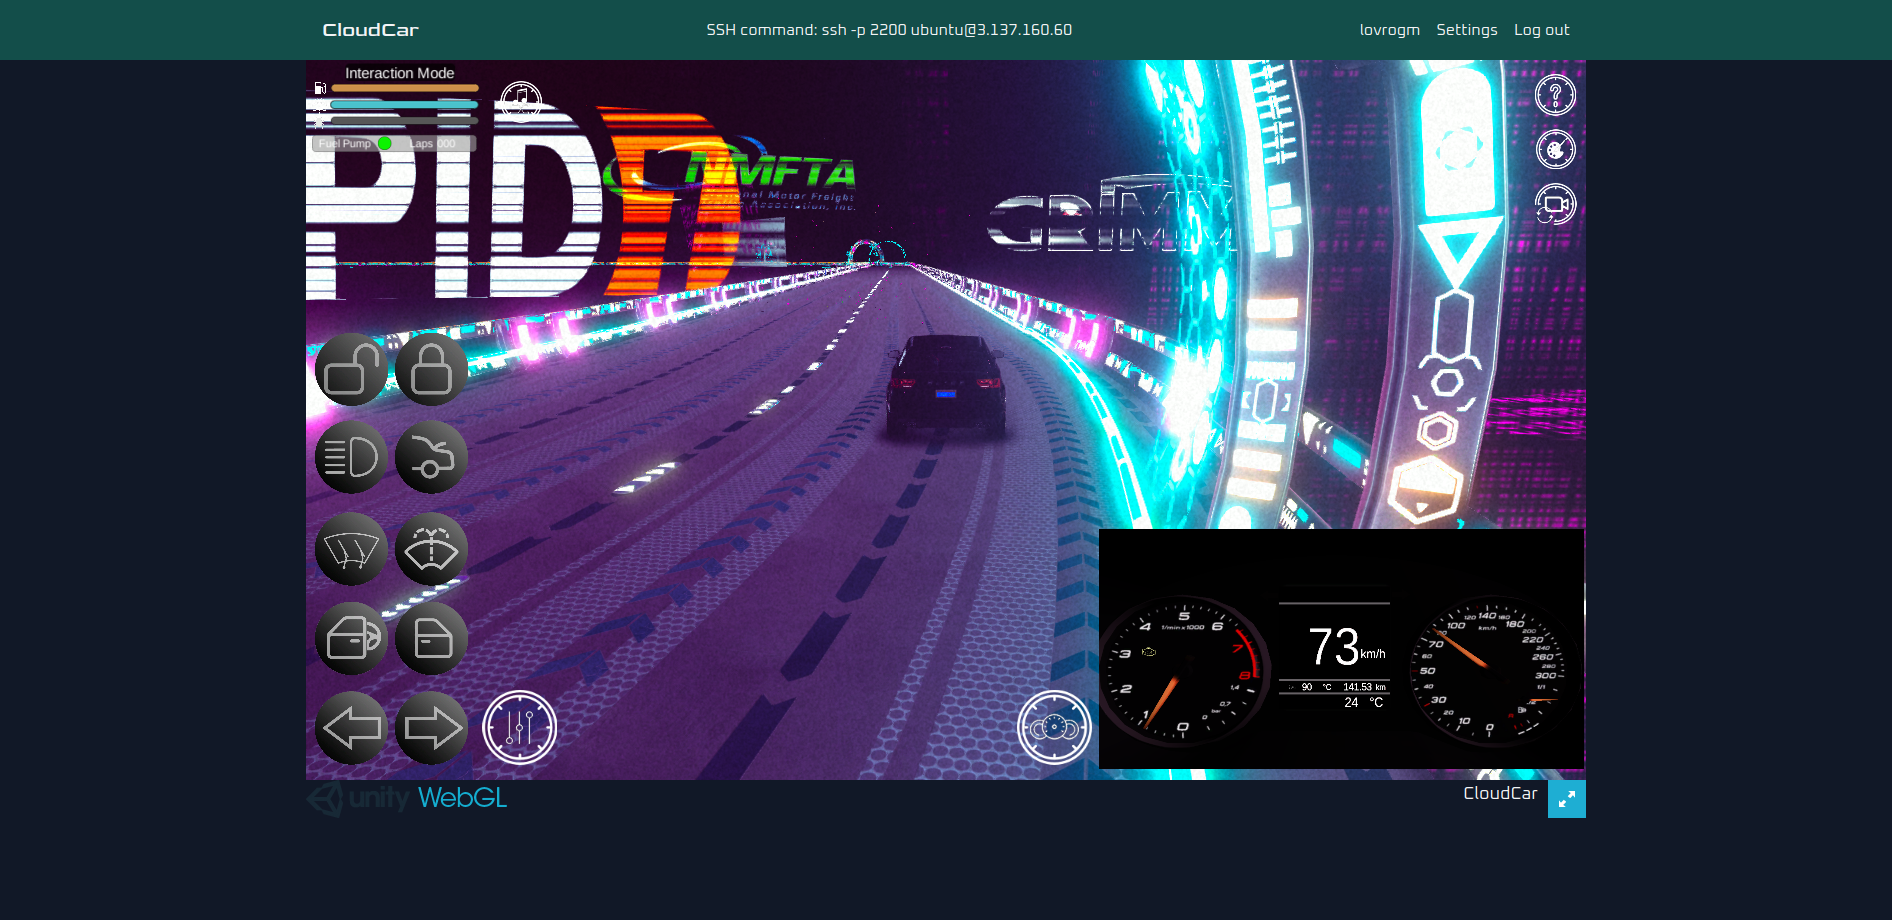
\includegraphics[width=\textwidth]{cloudcar.png}
\caption{Snimka zaslona - platforma CloudCar}
\label{fig:cloudcar}
\end{figure}

\newpage
Tijekom \textit{DEFCON30} konferencije održavalo se CTF natjecanje koje se bodovalo na dva načina: 
\begin{itemize}
    \item brojem odvoženih krugova na traci
    \item sakupljanjem zastavica 
\end{itemize}
Analizom CAN prometa moguće je bilo utvrditi koje CAN poruke određuju brzinu automobila, što su natjecatelji mogli iskoristiti kako bi odvozili veći broj krugova. Pojedinačne zastavice natjecatelji su mogli sakupiti analizom CAN prometa vezanih uz druge funkcije automobila.

Konkretni zadaci na platformi više ne postoje, ali je još uvijek moguće pristupiti simulaciji i analizirati CAN poruke određenih funkcija automobila.

\section{Simulatori}
\subsection{ICSim}
ICSim je simulator ploče s instrumentima koji radi povrh jednog \textit{SocketCAN} sučelja. Sastoji se od programa koji prikazuje ploču s instrumentima i upravljačkog programa pomoću kojeg korisnik može upravljati prikazanom brzinom, vratima i pokazivačima smjera (slika \ref{fig:icsim}). Korisnik simulatora potom može koristiti alate kompatibilne sa \textit{SocketCAN} sučeljima kako bi analizirao generirani promet između upravljačkog programa i programa ploče s instrumentima. Umjesto korištenja grafičkog korisničkog sučelja upravljačkog programa, korisnik može koristiti i igraći upravljač. 

\begin{figure}[htb]
\centering
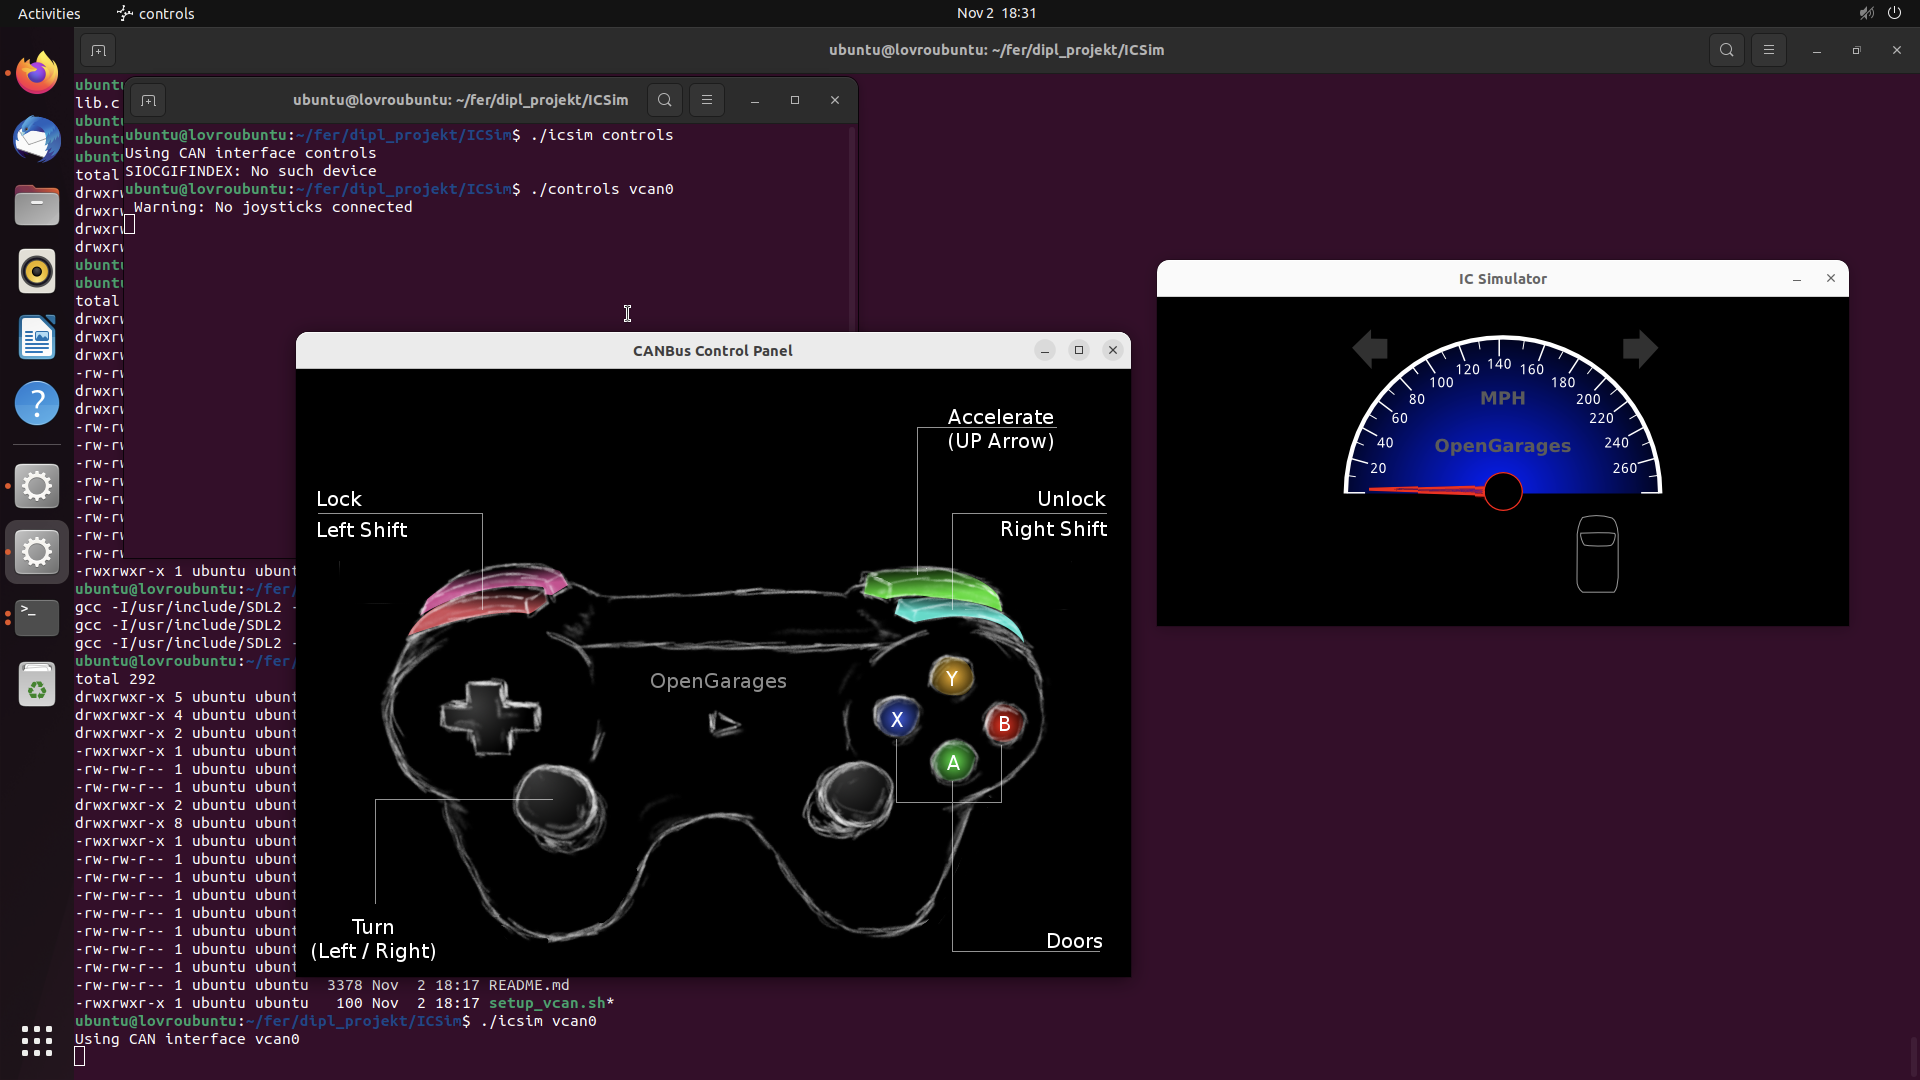
\includegraphics[width=370pt]{icsim.png}
\caption{Snimka zaslona - ICSim}
\label{fig:icsim}
\end{figure}

\subsection{Toyota PASTA}
\textit{Portable Automotive Security Testbed with Adaptability} (PASTA) razvili su Toyama et al. s podrškom korporacije \textit{Toyota Motor} \cite{toyama2018pasta, tsu2018pastagithub}. PASTA je fizički ispitni sustav otvorenog koda i sklopovlja, razvijen u svrhu omogućavanja edukacije i istraživanja sigurnosti na stvarnom sklopovlju prisutnom u automobilima. PASTA se sastoji od tri ECU-a odgovornih za domene pogonskog sklopa, šasije i kabine. ECU-ovi su povezani preko jednog središnjeg poveznika, a na središnji poveznik povezan je i OBD-II priključak. Svaki ECU je povezan na vlastiti zaslon koji prikazuje odgovarajuće informacije. Primjerice, ECU pogonskog sklopa na zaslonu prikazuje stanje prijenosa, kočenja, ubrzanja i orijentacije kotača. Ulaze ECU-ova čine fizička dugmad i sklopke kao i minijaturni upravljač automobila. Iako se može koristiti samostalno, PASTA je proširiva te moguće spojiti dodatne uređaje putem izloženog dijela CAN sabirnice. Navedena funkcionalnost demonstrirana je povezivanjem simulatora CARLA \cite{toyama2018pasta}. CARLA je simulator vožnje otvorenog koda izrađen u pogonskom sustavu \textit{Unreal Engine 4}, prvenstveno namijenjen za istraživanje pristupa autonomnoj vožnji \cite{dosovitskiy2017carla}. Simulator CARLA i sustav PASTA povezani su zasebnom \textit{Python} skriptom koja pretvara CAN poruke iz sustava PASTA u ulaze za simulator CARLA \cite{tsu2018pastacarla}.

\chapter{Implementacija sustava za obuku stručnjaka sigurnosti}
U sklopu ovog rada implementiran je proširivi sustav za stvaranje CTF zadataka, koji omogućava upoznavanje sadašnjih i budućih stručnjaka sigurnosti sa specifičnostima sustava u automobilima. Sustav je osmišljen i implementiran prema sljedećim zahtjevima:
\begin{enumerate}
    \item Sustav mora imati sposobnost simulacije komunikacijskih protokola i sustava specifičnih automobilima.
    \item Sustav mora biti implementiran programski, bez zahtjeva za dodatnim sklopovljem osim osobnog računala.
    \item Sustav mora omogućavati stvaranje novih CTF zadataka.
    \item Sustav mora biti programski proširiv.
    \item Sustav mora biti poveziv sa stvarnim sklopovljem.
    \item Sustav mora imati mogućnost pokretanja na osobnom računalu, ali i biti dostupan s udaljenog računala.
\end{enumerate}

Zahtjevi sustava definirani su prema prednostima i nedostatcima postojećih sustava opisanih u četvrtom poglavlju. Platforme VSEC i \textit{CloudCar} podržavaju udaljeno spajanje u svrhu CTF natjecanja, ali nije ih moguće pokretati lokalno na računalu, kao ni proširivati ni programski niti sa stvarnim sklopovljem te ne olakšavaju stvaranje novih zadataka. Sustav PASTA ispunjava većinu zahtjeva, ali zahtjeva posjedovanje sklopovlja kao i predznanja za sastavljanje sklopovlja sustava, što ga čini manje pristupačnim u odnosu na ostale sustave. Glavni doprinos implementiranog sustava je robustan način simuliranja sustava specifičnih automobilima i stvaranja CTF zadataka. Implementirani sustav namijenjen je za simulaciju CAN-a automobila, od sloja podatkovne poveznice do aplikacijskog sloja, s proizvoljnim brojem CAN sabirnica i ECU-ova.
\section{Korištene tehnologije}
\subsection{SocketCAN}
\textit{SocketCAN} je implementacija protokola CAN, CAN-FD i ISO-TP za Linux, koja omogućava korištenje CAN sklopovlja putem \textit{Berkley socket} API-ja\cite{socketcan}. Prije \textit{SocketCAN} paketa, komunikacija između korisničkih programa i CAN sklopovlja odvijala se izravno kroz upravljačke programe. Pritom je pri razvoju korisničkih programa bilo potrebno pisati više puta funkcionalno isti kod, za svaku podržanu vrstu CAN sklopovlja te voditi računa o specifičnostima njihovih upravljačkih programa. \textit{SocketCAN} apstrahira korištenje upravljačkih programa kroz \textit{Berkley socket} API te ih implementira kao mrežna sučelja. Ovakva implementacija donosi i prednosti korištenja Linux mrežnog stoga, poput redova okvira \engl{queueing of frames} i mogućnosti implementacije transportnih protokola u jezgri umjesto u korisničkom \engl{user space} kodu.

Temeljna ideja za ostvarivanje CAN komunikacije procesa je korištenje virtualnih \textit{SocketCAN} sučelja kao svojevrsnih CAN sabirnica. Virtualna CAN sučelja omogućena su upravljačkim programom \textit{vcan} te se ponašaju kao uobičajena \textit{loopback} sučelja te se zbog tog svojstva mogu koristiti za komunikaciju između procesa (engl. \textit{inter-process communication}, IPC). Prednost ovog pristupa je i kompatibilnost s ostalim alatima kompatibilnima sa \textit{SocketCAN} sučeljima, poput cijelog \textit{can-utils} paketa te alata za istraživanje sigurnosti automobila \textit{caringcaribou}. 

Komunikaciju između procesa putem \textit{vcan} sučelja, moguće je demonstrirati alatima \textit{cansend} i \textit{candump} iz paketa \textit{can-utils}. Alat \textit{candump} služi za ispis svih poruka na specificiranom \textit{SocketCAN} sučelju, a \textit{cansend} za slanje CAN poruka putem istog. Prvo je potrebno stvoriti i podići vcan sučelje korištenjem alata \textit{ip} (Ispis \ref{lst:vcan1}). Potom je potrebno pokrenuti prvo alat \textit{candump} pa alat \textit{cansend} i predati im proizvoljnu poruku i podignuto \textit{vcan} sučelje (Ispis \ref{lst:vcan2}).
\newpage
\begin{lstlisting}[style=terminal, label={lst:vcan1},caption={Stvaranje i podizanje \textit{vcan} sučelja}]
$ ip link add vcan0 type vcan
$ ip link set dev vcan0 up
$ ip a

(...)

7: vcan0: <NOARP,UP,LOWER_UP> mtu 72 qdisc noqueue state UNKNOWN group default qlen 1000
    link/can 
\end{lstlisting}
\begin{lstlisting}[style=terminal, label={lst:vcan2},caption={IPC putem \textit{vcan} sučelja}]
// Naredbeni redak 1
$ cansend vcan0 123#ABCD
$ cansend vcan0 123#EF01

// Naredbeni redak 2
$ candump vcan0
  vcan0  123   [2]  AB CD
  vcan0  123   [2]  EF 01
\end{lstlisting}

Isti pristup komunikaciji između procesa koristi i prethodno opisani sustav \textit{ICSim} te je skalabilan na veći broj procesa odnosno ECU programa.

\subsection{Docker i Docker Compose}
\textit{Docker} je platforma otvorenog koda koja omogućava pakiranje aplikacija u kontejnere, kako bi bile prenosive i izolirane od sustava na kojem se pokreću. Ključna komponenta \textit{Dockera} je \textit{Docker Engine} koja upravlja kontejnerima, slikama, mrežama i volumenima pohrane. 

Kontejnerizacija aplikacije vrši se kroz \textit{Dockerfile} tekstualne datoteke, koje definiraju potrebne korake za izgradnju izvršne datoteke, instalaciju potrebnih biblioteka te pokretanje aplikacije. Potom se iz \textit{Dockerfile} datoteke gradi \textit{Docker} slika koja sadrži sve potrebno za pokretanje aplikacije na sustavu za koji je izgrađena. Iz slike stvara se \textit{Docker} kontejner te se aplikacija pokreće u izoliranom okruženju, skoro potpuno odvojenom od sustava domaćina kroz mehanizme jezgre. \textit{Docker Engine} upravlja životnim ciklusom kontejnera te oslobađa korištene resurse nakon njihova uklanjanja. Uz navedeno, \textit{Docker Engine} upravlja umrežavanjem kontejnera stvaranjem potrebnih sučelja i dodavanjem pravila usmjeravanja paketa.

\textit{Docker Compose} je alat za definiranje i pokretanje aplikacija koje se sastoje od više kontejnera. \textit{Docker Compose} omogućava korisnicima korištenje YAML datoteku za definiranje usluga, mreža i volumena potrebnih za aplikaciju te njihovo pokretanje jednom naredbom.

\section{Opis sustava}
Sustav za stvaranje CTF zadataka, implementiran je kroz 4 komponente:
\begin{itemize}
    \item generatorsku skriptu
    \item dodatak Docker mrežnom upravljačkom programu \textit{dockercan}
    \item predložak programa ECU-a
    \item vizualnu komponentu \textit{ic-tui}
\end{itemize}

Kao temelj sustava odabrane su tehnologije \textit{Docker} i \textit{Docker Compose}. Svaki ECU program izoliran je u zasebni kontejner, a međusobno su povezani kroz \textit{Docker} mreže, gdje svaka mreža predstavlja jednu sabirnicu. Korištenje \textit{Docker} kontejnera i mreža, omogućava definiranje CTF zadataka kroz YAML konfiguracije \textit{Docker Composea}, što osigurava njihovo lakše pokretanje, kao i robusnost upravljanja mrežama kontejnera i resursima domaćinskog sutava neizravno putem \textit{Docker Enginea}.

S obzirom na to da Docker podržava samo komunikaciju putem protokola TCP i UDP, napisan je dodatak Docker mrežnom upravljačkom programu \engl{Docker network driver plugin}, nazvan \textit{dockercan}. Dodatak \textit{dockercan} koristi se za umrežavanje kontejnera pomoću \textit{SocketCAN} sučelja i alata te omogućava CAN i CAN-FD \textit{broadcast} komunikaciju između kontejnera u istoj mreži. Mreže stvorene dodatkom \textit{dockercan} simuliraju CAN sabirnice.

Napisan je i predložak programa ECU-a, koji omogućava lakše stvaranje višedretvenog programa koji može asinkrono komunicirati i odgovarati na poruke putem protokola CAN, CAN-FD, UDS i XCP. Uz navedeno, predložak ima mogućnost definiranja komunikacije prema drugim kontejnerima putem uobičajenih \textit{Docker} mreža. Primjerice, prema kontejneru koji sadrži GUI za vizualizaciju nekog sustava automobila ili kontejneru s posredničkim programom za integraciju s simulatorom poput simulatora CARLA.

Primjer programa koji je kompatibilan s predloškom programa ECU-a je vizualna komponenta \textit{ic-tui}. Komponenta \textit{ic-tui} je program koji prikazuje glavne elemente ploče s instrumentima putem korisničkog sučelja naredbenog retka (engl. \textit{terminal user interface}, TUI). Pruža HTTP API za ažuriranje prikazanih vrijednosti s kojim ECU predložak može komunicirati. Uz to, može se pokretati i u SSH načinu rada, što omogućava udaljeno spajanje na TUI.

Sustav je objedinjen generatorskom skriptom, koja služi kao vodič za inicijalno postavljanje projekta CTF zadatka, kojeg korisnik potom može modificirati svojim kodom. Skripta generira i \textit{Docker Compose} YAML datoteku, koja definira \textit{dockercan} mreže te ECU i druge kontejnere koji su dio zadatka.

\subsection{Primjer arhitekture generiranog zadatka }
Slika \ref{fig:arhitekturasustava} prikazuje arhitekturu s osam ECU-ova povezanih na 3 CAN sabirnice, odnosno 8 kontejnera povezanih u 3 \textit{dockercan} mreže. Dva ECU-a poveznika nalaze se u više mreža, odnosno poveznik AC u mrežama A i C te poveznik ABC u sve tri definirane mreže, ali njihovo konkretno ponašanje definira korisnik. Primjerice, mreže A, B i C bi u svrhu CTF zadatka mogle predstavljati CAN sabirnice domene šasije, kabine i pogonskog sklopa, a poveznici imaju svrhu prosljeđivanja određenog skupa poruka između sabirnica.

\begin{figure}[htb]
\centering
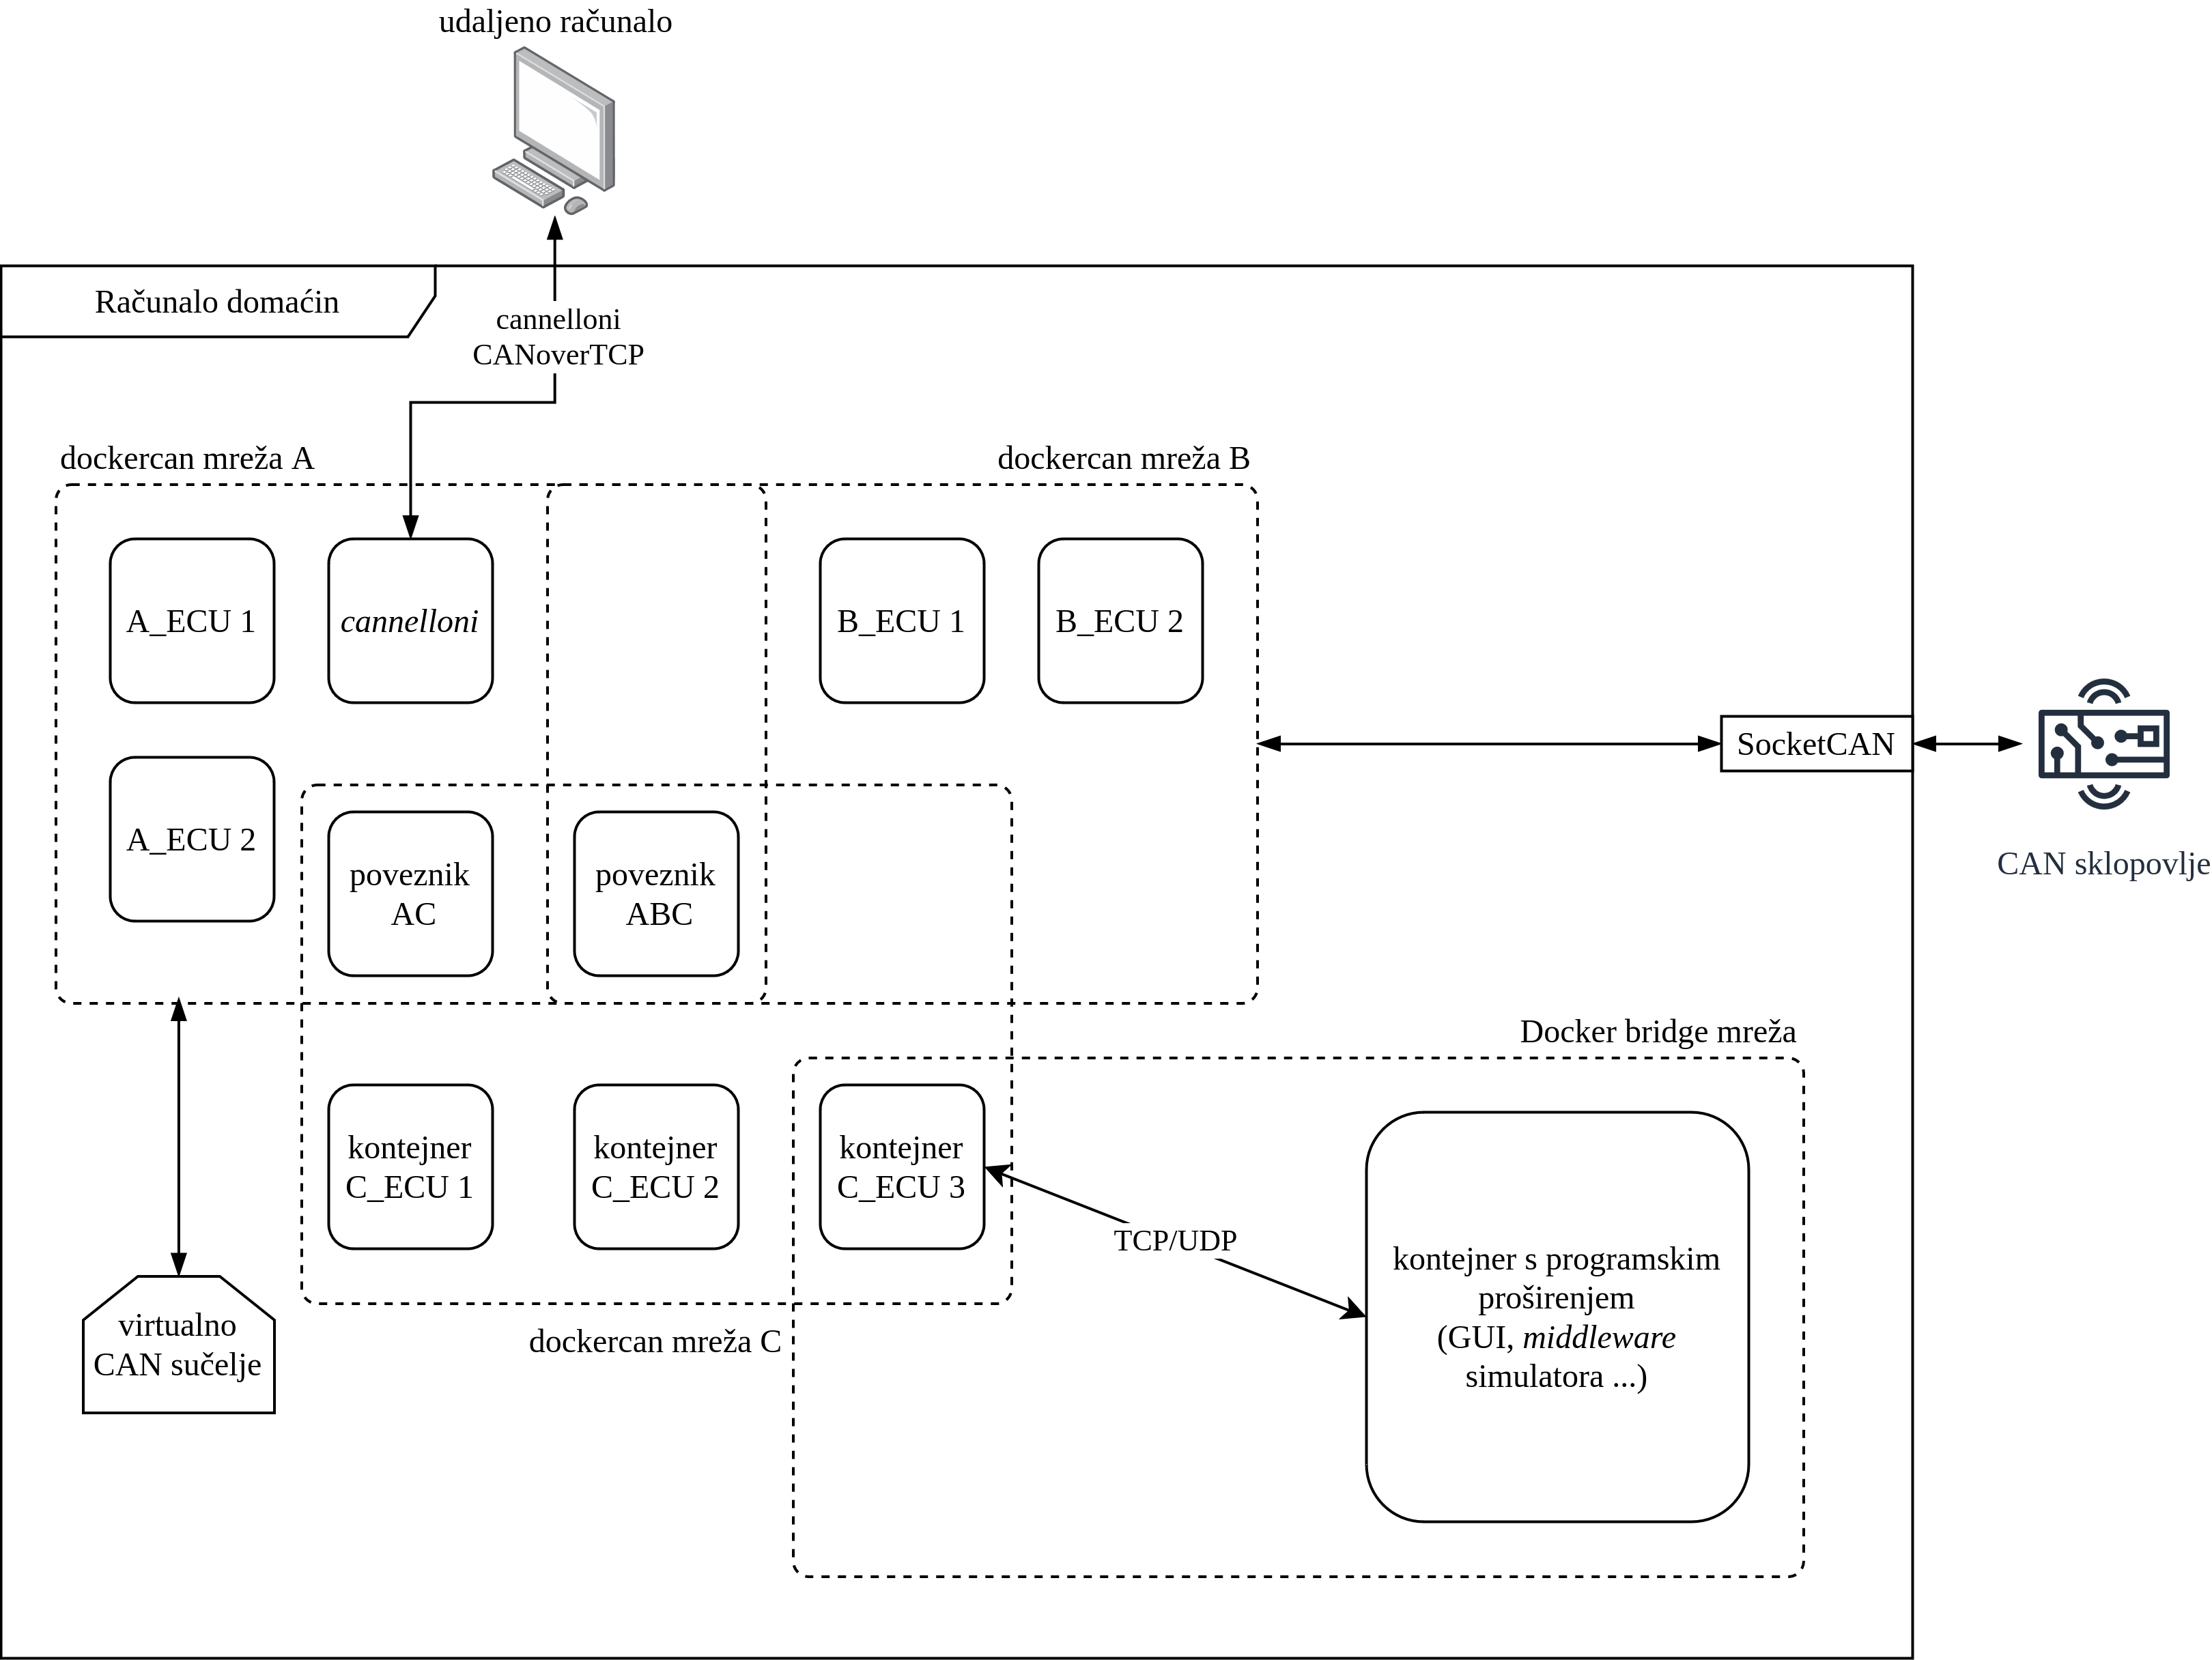
\includegraphics[width=\textwidth]{arhitektura2.png}
\caption{Arhitektura sustava}
\label{fig:arhitekturasustava}
\end{figure}

Konkretna tehnička izvedba dodatka \textit{dockercan} opisana je u poglavlju \ref{sec:dockercan}, ali potrebno je naglasiti da ima opciju stvaranja virtualnog CAN sučelja na domaćinskom računalu, kako bi se osobi koja rješava zadatak omogućio pristup određenoj CAN sabirnici. Navedeno je prikazano na \textit{dockercan} mreži A spajanjem vanjskog CAN sučelja. Uz to, izvedba dodatka \textit{dockercan} s pomoću \textit{SocketCAN} mrežnih sučelja i alata, omogućava spajanje vanjskog CAN sklopovlja na mrežu. Navedeno je prikazano na primjeru \textit{dockercan} mreže B.

Ukoliko je potrebno omogućiti udaljeno spajanje na \textit{dockercan} mrežu, moguće je koristiti alat \textit{cannellonni}. Alat \textit{cannellonni} omogućava udaljeno spajanje dvaju \textit{SocketCAN} sučelja putem TCP, UDP i SCTP protokola \cite{reinhardt2015mapping}. U generatorskoj skripti je predviđena mogućnost dodavanja prethodno konfiguriranog \textit{cannellonni} kontejnera u svrhu udaljenog spajanja na neku \textit{dockercan} mrežu.
\newpage
Naposljetku, za komunikaciju s potencijalnim programskim proširenjima predviđeno je povezivanje ECU kontejnera s kontejnerima proširenja putem uobičajenih \textit{Docker bridge} mreža. Programsko proširenje može biti \textit{web} aplikacija koja prikazuje status rješavanja zadatka, interaktivno grafičko korisničko sučelje nalik programu upravljaču iz sustava \textit{ICSim} ili program posrednik za povezivanje zadatka na simulator poput simulatora CARLA.

\section{Predložak programa ECU-a}
U svrhu olakšavanja izrade programa ECU-a za CTF zadatke stvoren je predložak koji služi kao početna točka. Predložak korisniku omogućava definiranje ponašanja ECU-a i odgovora na UDS, XCP i CAN poruke kroz 5 \textit{Python} datoteka.

Predložak se sastoji od direktorija \texttt{ecu\_template}, \texttt{impl} i datoteke \texttt{main.py}. Direktorij \texttt{ecu\_template} sadrži interni kod predloška potrebnog za njegovu normalnu funkciju. Direktorij \texttt{impl} sadrži datoteke \texttt{can\_handler.py}, \texttt{uds\_handler.py} i \texttt{xcp\_handler.py} u kojima korisnik može definirati željeno ponašanje u pogledu navedena tri protokola. Uz njih, u direktoriju \texttt{impl}, nalazi se datoteka \texttt{ecu\_model.py} koja služi za održavanje stanja ECU-a između prethodne tri datoteke, kao i za definiranje ponašanja ovisnog o promjeni stanja. Predložak objedinjuje datoteka \texttt{main.py} koja postavlja i pokreće program ECU-a.

\subsection{Biblioteka Scapy i SocketCAN}
Pri implementaciji predloška programa ECU-a, odabrana je biblioteka \textit{Scapy}\cite{scapy}. Odabrana je zbog mogućnosti parsiranja poruka niza komunikacijskih protokola specifičnih automobilima, kao i zbog kompatibilnosti sa \textit{SocketCAN} sučeljima. Razmatrane su i biblioteke \textit{python-can} te \textit{can-isotp}, zbog mogućnosti definiranja \textit{callback} funkcija koje se pozivaju po primitku \textit{CAN} poruka \cite{pythoncan,canisotp}. Međutim, \textit{Scapy} podržava parsiranje poruka većeg broja protokola, poput UDS-a i XCP-a, koji u navedenim bibliotekama nisu podržani. Uz to, \textit{Scapy} u potpunosti iskorištava mogućnosti \textit{SocketCANa}, poput podrške za transportni protokol ISO-TP u \textit{Linux} jezgri. Navedeno svojstvo \textit{Scapy} čini kompatibilnijim s ostalim \textit{SocketCAN} alatima, u odnosu na biblioteku \textit{can-isotp}, koja ISO-TP implementira programski u \textit{Pythonu}, povrh jezgre.

\textit{Scapy} nudi način korištenja kroz naredbeni redak, kroz vlastiti omotač oko \textit{Python} ljuske. Primjerice, za stvaranje objekta razreda \texttt{CANSocket} u svrhu slanja i primanja poruka putem \textit{SocketCAN} sučelja dovoljno je pokrenuti naredbe s linija 1 do 3, iz ispisa \ref{lst:cansocket}. Linijom 1 omogućava se korištenje \textit{SocketCANa} izravno, umjesto putem biblioteke \textit{python-can}, a linijom 2 učitava se modul \texttt{cansocket}. Linijom 3 stvoren je \texttt{CANSocket} objekt za slanje i primanje poruka putem virtualnog CAN sučelja \texttt{vcan0}. Parametrom \texttt{can\_filters} definirano je filtriranje svih CAN paketa osim onih s arbitražnim identifikatorom \texttt{0x344}. Filtriranje se odvija na razini \textit{SocketCAN socketa} te je konfigurirano kroz \textit{setsockopt} pozive \cite{socketcan}. Slanje jedne CAN poruke i blokirajuće čitanje iduće poruke moguće je ostvariti kroz pozive metoda \texttt{send} i \texttt{recv} ili kroz jedan poziv metode \texttt{sr1}, prikazano na linijama 5 do 7.   
\newpage
\begin{lstlisting}[language=Python, label={lst:cansocket},caption={Korištenje \textit{SocketCAN} sučelja iz ljuske alata \textit{Scapy}}]
conf.contribs['CANSocket'] = {'use-python-can': False}
load_contrib('cansocket')
socket = CANSocket(channel="vcan0", can_filters=[{'can_id': 0x344, 'can_mask': 0x7FF}])

socket.sr1(CAN(identifier=0x345, data=b'\x01\x02\x03'))
# ili
socket.send(CAN(identifier=0x345, data=b'\x01\x02\x03'))
socket.recv()
\end{lstlisting}

U praksi, metoda \texttt{sr1} korisnija je za protokole oblika \textit{zahtjev-odgovor}, primjerice za protokol UDS. Razlog tomu je što Scapy rekurzivno provjerava \texttt{answers} metodu implementiranu na razredima pojedinačnih tipova paketa, od nižih prema višim slojevima OSI modela. Primjerice, u slučaju poslanog \texttt{UDS\_DSC} paketa, odnosno zahtjeva za servisom \texttt{DiagnosticSessionControl}, \textit{Scapy} će pozvati \texttt{answers} metodu svakog idućeg primljenog paketa. Metodi \texttt{answers} će predati poslani paket kao parametar, kako bi mogla usporediti sadržaje oba paketa i zaključiti odgovara li primljeni paket na poslani. U slučaju da je primiljen paket \texttt{UDS\_DSCPR}, koji je odgovor na poslani \texttt{UDS\_DSC}, pozvana će biti metoda \texttt{answers} paketa \texttt{UDS\_DSCPR} koja provjerava je li tip dijagnostičke sesije isti u poslanom i primljenom paketu (ispis \ref{lst:dscpr}). Ukoliko je, \textit{Scapy}, primljeni paket će biti vraćen iz poziva \texttt{sr1} metode. Potrebno je napomenuti da je poziv metode \texttt{UDS\_DSCPR.answers}, posljednji u nizu rekurzivnih poziva te da joj je prethodio poziv \texttt{UDS.answers}. 
\bigskip
\begin{lstlisting}[language=Python, label={lst:dscpr},caption={\texttt{UDS\_DSCPR.answers}metoda}]
class UDS_DSCPR(Packet):
    name = 'DiagnosticSessionControlPositiveResponse'
    fields_desc = [
        ByteEnumField('diagnosticSessionType', 0,
                      UDS_DSC.diagnosticSessionTypes),
        StrField('sessionParameterRecord', b"")
    ]

    def answers(self, other):
        return isinstance(other, UDS_DSC) and \
            other.diagnosticSessionType == self.diagnosticSessionType
\end{lstlisting}

\textit{Scapy} UDS paketi formiraju se korištenjem operatora "/" za slaganje slojeva. U slučaju UDS-a, kao temeljni sloj koristi se razred \texttt{UDS} povrh kojeg se nadodaju specifični tipovi UDS zahtjeva ili odgovora. Sastavljanje i slanje pakta zahtjeva UDS \texttt{ReadMemoryByAddress} koji čita \texttt{0xFF} okteta početka memorije prikazano je linijama 2 i 3 u ispisu \ref{lst:udspkt}, a linijom 7 poslan je pozitivan odgovor na zahtjev iz druge ljuske. Primljeni paket je instanca temeljnog \texttt{UDS} razreda, a konkretnom UDS odgovoru moguće je pristupiti putem člana \texttt{payload}. Specifičnim poljima odgovora također je moguće pristupiti putem članova razreda. U slučaju servisa \texttt{ReadMemoryByAddress} vraćenom dijelu memorije pristupa se putem člana \texttt{dataRecord}.
\bigskip
\begin{lstlisting}[language=Python, label={lst:udspkt},caption={Sastavljane \textit{Scapy} paketa}]
# ========= Scapy ljuska A =========
>>> pkt = UDS()/UDS_RMBA(memoryAddressLen=4,memorySizeLen=1,memoryAddress4=0x0, memorySize1=0xFF)
>>> res = s.sr1(pkt)

# ========= Scapy ljuska B ========= 

>>> s.send(UDS()/UDS_RMBAPR(dataRecord=b"diplomski"))
10

# ========= Scapy ljuska A =========
>>> res.payload
<UDS_RMBAPR  dataRecord='diplomski' |>
>>> res.dataRecord
b'diplomski'

\end{lstlisting}

\subsection{Definiranje CAN, UDS i XCP aplikacijske logike}

Svaka od datoteka \texttt{can\_handler.py}, \texttt{uds\_handler.py} i \texttt{xcp\_handler.py}, sadrži odgovarajući razred \engl{class} koji korisnik može implementirati, ako želi definirati aplikacijsku logiku u kontekstu nekog od navedenih protokola.

Primjerice, za definiranje CAN aplikacijske logike, korisnik treba implementirati razred \texttt{CANHandlerImpl}. Razred \texttt{CANHandlerImpl} nasljeđuje apstraktni razred \texttt{CanHandler} koji sadrži neimplementiranu metodu \texttt{handle\_msg}. Navedena metoda je \textit{callback} metoda koja se poziva pri svakom primitku CAN poruke. Primljena CAN poruka prosljeđuje se metodi \texttt{handle\_msg} kroz argument \texttt{msg}. Apstraktni razred \texttt{CanHandler} sadrži i referencu na \texttt{NativeCANSocket} instancu, kako bi svaki razred koji ga nasljeđuje mogao odgovarati na ili slati CAN poruke. Primjer jednostavnog \texttt{CanHandlerImpl} razreda koji sve primljene CAN poruke ponovno šalje s arbitražnim identifikatorom uvećanim za 1, prikazan je ispisom \ref{lst:canhandler}. Opisana struktura razreda vrijedi i za datoteke \texttt{uds\_handler.py} i \texttt{xcp\_handler.py}, odnosno razrede \texttt{UDSHandlerImpl} i \texttt{XCPHandlerImpl}.
\bigskip
\begin{lstlisting}[language=Python, label={lst:canhandler},caption={\texttt{CanHandlerImpl} primjer}]
class CanHandlerImpl(CanHandler):
    def __init__(self, ecu: ECUModelImpl):
        super().__init__(ecu)

    def handle_msg(self, msg: CAN):
        print(msg.identifier)
        msg.identifier += 1
        self.socket.send(msg)
\end{lstlisting}

U slučaju implementacije razreda \texttt{UDSHandlerImpl}, preporučeni obrazac je korištenje \textit{Python} \texttt{match-case} mehanizma za razlikovanje različitih vrsta UDS zahtjeva (ispis \ref{lst:udshandler}). Prikazani primjer odgovara pozitivnim odgovorom na svaki zahtjev za servisima \texttt{ECUReset} te \texttt{DiagnosticSessionControl}.
\bigskip
\begin{lstlisting}[language=Python, label={lst:udshandler},caption={\texttt{UDSHandlerImpl} primjer}]
class UDSHandlerImpl(UDSHandler):
    def __init__(self, ecu: ECUModel):
        super().__init__(
            ecu,
        )

    def handle_msg(self, msg: UDS):
        match msg.payload:
            case UDS_ER():
                self.isotp.send(UDS() / UDS_ERPR(resetType=msg.resetType))
            case UDS_DSC():
                self.isotp.send(
                    UDS() / UDS_DSCPR(diagnosticSessionType=msg.diagnosticSessionType)
                )
\end{lstlisting}
Kako bi nepotrebni pozivi \textit{callback} metoda bili izbjegnuti u \texttt{config.py} datoteci moguće je definirati filtriranje CAN poruka prema arbitražnom identifikatoru za metode \texttt{handle\_msg} razreda \texttt{CANHandlerImpl} i \texttt{XCPHandlerImpl} (ispis \ref{lst:configpy}). Parametar \texttt{can\_mask} sadržava masku kojom se određuju bitovi identifikatora relevantni za filtriranje. Postavljanjem parametra na \texttt{0x7FF} ili \texttt{0b11111111} binarno, odabiru se svi bitovi 11-bitnog identifikatora. Uz navedeno, u \texttt{config.py} datoteci potrebno je definirati ISO-TP adresu UDS poslužitelja u obliku \textit{Python} rječnika s vrijednostima \texttt{rx\_id} i \texttt{tx\_id}. Onemogućavanje protokola moguće je postavljanjem varijabli \texttt{CAN\_FILTERS}, \texttt{XCP} i \texttt{UDS} na vrijednost \texttt{None}. 
\bigskip
\begin{lstlisting}[language=Python, label={lst:configpy},caption={\texttt{Konfiguracija filtriranja i ISO-TP adrese} primjer}]

CAN_FILTERS = [
    {"can_id": 0x456, "can_mask": 0x7FF},
]

XCP = [
    {"can_id": 0x701, "can_mask": 0x7FF},
]

UDS = dict(rx_id=0x100, tx_id=0x101)
\end{lstlisting}

\subsection{Definiranje stanja ECU-a}
Datoteka \texttt{ecu\_model.py} i razred \texttt{ECUModelImpl} koji definira, namijenjen je pohranjivanju stanja. Stoga svaki od navedenih razreda za definiranje aplikacijske logike protokola CAN, UDS i XCP, čuva i referencu na instancu razreda \texttt{ECUModelImpl}.

Korisniku je prepušteno koje će konkretno podatke o stanju čuvati u instanci razreda \texttt{ECUModelImpl}. Dodatno apstraktni razred \texttt{ECUModel} omogućava dodavanje i uklanjanje promatrača metodama \texttt{attach\_listener} i \texttt{detach\_listener} te njihovo obavještavanje metodom \texttt{notify}. Prikazan je primjer implementacije jednostavnog ECU-a, koji čita brzinu vozila sa sabirnice te ju šalje HTTP POST zahtjevom na nedefinirani API (ispis \ref{lst:stanje}). Promatrače je potrebno postaviti u predefiniranoj funkciji \texttt{setup\_ecu\_model}, koju će izvršiti glavni program prilikom pokretanja.

\newpage
\begin{lstlisting}[language=Python, label={lst:stanje},caption={Primjer implementacije \texttt{ECUModelImpl}}]
class CanHandlerImpl(CanHandler):
    def __init__(self, ecu: ECUModelImpl):
        super().__init__(ecu)

    class SpeedData:
        def __init__(self, data: bytes):
            self.speed = int.from_bytes(data[1:3])

    def handle_msg(self, msg: CAN):
        if msg.data[0] == 0xAB and msg.length == 3:
            speed_data = SpeedData(data=msg.data)
            if 0 < speed_data.speed <= 250:
                self.ecu.set_speed(speed_data.speed)

class ECUModelImpl(ECUModel):        
    class APIListener(Listener):
        def update(self, model: ECUModelImpl):
            data = {
                "speed": model.speed,
            }
    
            try:
                print("sending req")
                requests.post("http://api:8080/update", json=data)
            except Exception as e:
                print(e)
    def __init__(self):
        super().__init__()
        self.speed = 0
    def set_speed(self, speed: int):
        self.speed = speed
        self.notify()

def setup_ecu_model():
    model = ECUModelImpl()
    model.attach_listener(APIListener())
    return model
\end{lstlisting}

\section{Vizualna komponenta zadataka}
U svrhu vizualizacije zadataka te prikazivanja povratne informacije natjecatelju, izrađena je vizualna komponenta. Za vizualnu komponentu odabrana je ploča s instrumentima te je implementirana kao korisničko sučelje naredbenog retka (engl. \textit{terminal user interface}, TUI) (slika \ref{fig:ictui}). TUI je odabran zbog jednostavnosti implementacije te dostupnosti 
\begin{figure}[htb]
\centering
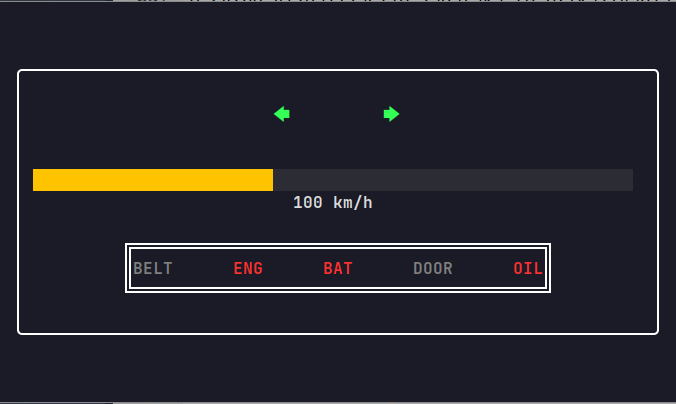
\includegraphics[width=\textwidth]{ictui.png}
\caption{TUI ploče s instrumentima}
\label{fig:ictui}
\end{figure}
\subsection{Implementacija}
Pri izradi vizualne komponente korištena je biblioteka \textit{Wish} i razvojni okvir \textit{Bubbletea} programskog jezika \textit{Go} \cite{wish, bubbletea}. Razvojni okvir \textit{Bubbletea} koristi se za stvaranje TUI aplikacija te definira niz jednostavnih često korištenih TUI komponenti. Primjerice, za prikaz brzinomjera na ploči s instrumentima, korištena je komponenta \texttt{progress}.

U sklopu \textit{Bubbletea} arhitekture, vizualna komponenta koristi \textit{Go} dretve \engl{goroutines} za pokretanje jednostavnog HTTP servera koji očekuje POST zahtjev s stanjem ploče koje treba prikazati. Prikazan je primjer zahtjeva upućenog alatom \textit{curl}, pod pretpostavkom da je komponenta pokrenuta na istom računalu (ispis \ref{lst:curl}). U slučaju da ECU program treba signalizirati da je ostvaren uvjet za pobjedu te da je potrebno prikazati zastavicu, može to učiniti korištenjem \texttt{winCondition} paramtera, nakon čega će se umjesto ploče s instrumentima prikazati zastavica.
\bigskip
\begin{lstlisting}[style=terminal, label={lst:curl},caption={Primjer POST zahtjeva sa stanjem ploče s instrumentima}]
$ curl -X POST -H "Content-Type: application/json" --data \
'{"winCondition":false, \ 
  "speed":100 , \ 
  "blinkers":true, \
  "seatbelt":false, \
  "engine":true, \
  "battery":true, \
  "doors":false, \ 
  "oil":true}' localhost:8080/update
\end{lstlisting}

Udaljeni prikaz TUI-ja ostvaren je kroz biblioteku \textit{Wish}, koja omogućava prikaz \textit{Bubbletea} TUI aplikacija putem SSH-a te u tu svrhu implementira vlastiti SSH server. Implementirana vizualna komponenta podržava zastavice "-ssh" i "-a", a upute je moguće ispisati postavljanjem zastavice "-h" (ispis \ref{lst:ictui_usage}). Zastavica "-ssh" koristi se za pokretanje vizualne komponente u sklopu \textit{Wish} servera, a zastavica "-a" omogućava specificiranje adrese i pristupa na kojima će HTTP poslužitelj slušati.
\bigskip
\begin{lstlisting}[style=terminal, label={lst:ictui_usage},caption={Korištenje vizualne komponente}]
$ ./ic-tui -h
Usage of ./ic-tui:
  -a string
    	Address and port for HTTP API in format <ip_address>:<port> (default ":8080")
  -ssh
    	Set to run as a Wish SSH server

$ ./ic-tui -a "0.0.0.0:4000" -ssh
\end{lstlisting}
\newpage
\section{Dodatak Docker mrežnom upravljačkom programu} \label{sec:dockercan}
Pri implementaciji sustava za stvaranje CTF zadataka, bilo je potrebno ostvariti pouzdan način umrežavanja ECU programa odnosno ECU kontejnera te su razmotrene sljedeće opcije:
\begin{itemize}
    \item umetanje skripti za umrežavanje u svaki kontejner
    \item umrežavanje putem klasičnih \textit{Docker} mreža te tuneliranje CAN prometa putem TCP-a
    \item zasebni program koji brine o umrežavanju i stanju kontejnera
\end{itemize}

Opcija umetanja skripti kroz \textit{Dockerfile}, koje se pokreću na početku rada kontejnera te ga povezuju putem \textit{SocketCAN} mrežnih sučelja i pravila usmjeravanja, pokazala se nepouzdanom. Nedostatak centralnog entiteta, dovodio je do problema u sinkronizaciji između kontejnera pri stvaranju mrežnih sučelja i pravila usmjeravanja. Uz navedeno, sam način umrežavanja nije pouzdan te ostavlja više prostora za korisničke pogreške.

Pouzdanija opcija bila je umrežavanje kontejnera putem klasičnih Docker mreža te tuneliranje CAN prometa između kontejnera putem TCP-a. Međutim, ova opcija zahtjeva pokretanje dodatnog programa za tuneliranje u svakom kontejneru, što kao i prethodna opcija ostavlja više prostora za korisničke pogreške. Uz navedeno, potrebno bi bilo osmisliti proces kojim će kontejneri međusobno iskomunicirati podatke poput TCP pristupa na kojima će tuneli biti postavljeni. Za više sabirnica ovaj postupak postaje višestruko kompleksniji.

Korištenje zasebnog programa koji brine o umrežavanju i stanju kontejnera najpouzdanija je opcija od prethodno navedenih. Međutim, navedeni program bi morao voditi računa i o uklanjanju stvorenih mrežnih sučelja i ostalih artefakata. Dodatno, istu funkciju već obavlja \textit{Docker Engine} te su naposljetku istražene opcije za njegovo proširenje.

\textit{Docker Engine} moguće je proširiti pisanjem i korištenjem mrežnih dodataka, dodataka za bilježenje dnevničkih zapisa te volumnih dodataka. Za potrebe omogućavanja novih vrsta umrežavanja, koriste se mrežni dodatci. Stoga je ova opcija odabrana kao pouzdan način omogućavanja umrežavanja ECU kontejnera putem protokola CAN.  

\subsection{Linux mrežni imenski prostori}
\textit{Linux} mrežni imenski prostori \engl{network namespaces}, pružaju mogućnost izolacije mrežnih resursa operacijskog sustava poput mrežnih sučelja i uređaja, mrežnih stogova, tablica usmjeravanja i sigurnosnih stijena \cite{man2024namespaces}. Mrežni imenski prostor služi kao potpuno izolirano mrežno okruženje za procese koji mu pripadaju. Dodavanje dvaju mrežnih imenskih prostora korištenjem alata \textit{ip}, prikazano je ispisom \ref{lst:ipns}.
\bigskip
\begin{lstlisting}[style=terminal, label={lst:ipns},caption={Dodavanje mrežnih imenskih prostora}]
$ ip netns add ns1
$ ip netns add ns2

$ ip netns
ns1
ns2
\end{lstlisting}
Navedena svojstva čine mrežne imenske prostore pogodnima za kontejnerizaciju aplikacija te je takav pristup mrežnoj izolaciji koristi \textit{Docker} \cite{rana2023dockernetworking}. Konkretnije, pri pokretanju svakog novog kontejnera, \textit{Docker} mu dodjeljuje novi mrežni imenski prostor. Ovim postupkom, izbjegavaju se potencijalne kolizije s drugim aplikacijama pri zauzimanju TCP i UDP pristupa te pri korištenju ostalih mrežnih resursa.

S obzirom na to da su kontejneri mrežno izolirani, za omogućavanje njihove međusobne komunikacije \textit{Docker} ih automatski dodaje u pretpostavljenu \textit{bridge} mrežu. Kako bi \textit{bridge} mreža ispravno funkcionirala, \textit{Docker} koristi dvije vrste mrežnih sučelja: \textit{bridge} i \textit{veth}. \textit{Linux} mrežno sučelje \textit{bridge} ponaša se kao virtualni preklopnik, prosljeđujući pakete između sučelja spojenih na njega. Mrežno sučelje \textit{veth} je lokalni \textit{Ethernet} tunel te služi za međusobno povezivanje mrežnih sučelja. Krajevi tunela su \textit{veth} parovi, gdje se svaki nalazi u zasebnom mrežnom imenskom prostoru. Korištenje samo sučelja \textit{veth} za međusobno povezivanje imenskih prostora svih kontejnera, rezultiralo bi u $\binom{n}{2}$ \textit{veth} tunela, gdje je $n$ broj kontejnera. Stoga \textit{Docker} koristi sučelje \textit{bridge} na računalu domaćinu, za usmjeravanje paketa između \textit{veth} tunela, što smanjuje broj tunela na $n$ (slika \ref{fig:bridge})
\begin{figure}[htb]
\centering
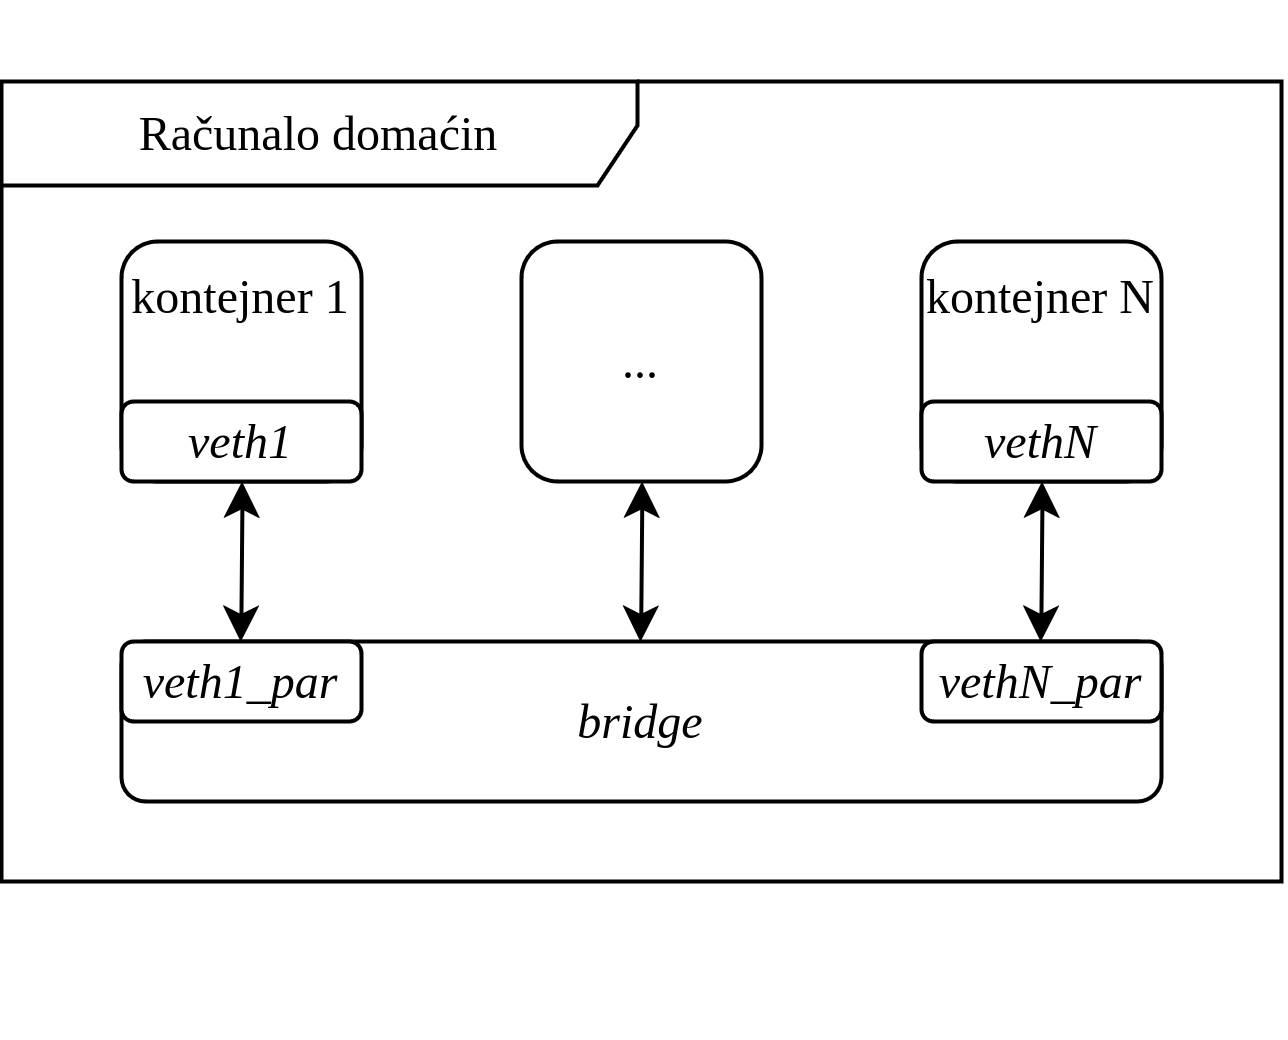
\includegraphics[width=250pt]{bridge.png}
\caption{\textit{Docker} bridge mreža}
\label{fig:bridge}
\end{figure}
\newpage
\subsection{Umrežavanje kontejnera korištenjem paketa SocketCAN} \label{sec:dockercan2}

\textit{SocketCAN} ekvivalent \textit{veth} tunelima su \textit{vxcan} tuneli, koja omogućavaju povezivanje \textit{Linux} mrežnih imenskih prostora putem protokola CAN, a time i povezivanje \textit{Docker} kontejnera \cite{liu2018interfaces}. Za prosljeđivanje CAN poruka između \textit{vcan} i \textit{vxcan} sučelja, koristi se jezgreni modul \textit{can\_gw} i pripadajući alat \textit{cangw}. Povezivanje dvaju imenskih prostora \texttt{ns1} i \texttt{ns2} \textit{vxcan} tunelom, prikazano je ispisom \ref{lst:vxcan1}. Povezivanjem mrežnih imenskih prostora $n$ kontejnera na ovaj način rezultira u $\binom{n}{2}$ \textit{vxcan} tunela, kao i u slučaju \textit{veth} tunela. 

\bigskip
\begin{lstlisting}[style=terminal, label={lst:vxcan1},caption={Povezivanje mrežnih imenskih prostora \textit{vxcan} tunelom}]
$ ip link add vxcan1 type vxcan peer name vxcan1_par

$ ip link set vxcan1 netns ns1
$ ip link set vxcan1_par netns ns2
\end{lstlisting}


\textit{SocketCAN} ekvivalent sučelju \textit{bridge} ne postoji te izravna preslika optimizacija iz slučaja \textit{veth} tunela nije moguća. Međutim, zbog \textit{loopback} svojstva virtualnih CAN sučelja \textit{vcan}, moguće ih je iskoristiti kao zamjenu za sučelje \textit{bridge}. Sučelje \textit{vcan} nije izvorno namijenjeno za ovu primjenu te nije moguće dodijeliti mu sučelja \textit{vxcan}, kao što je to moguće u slučaju sučelja \textit{bridge} i \textit{veth}. Opisano ograničenje moguće je zaobići korištenjem alata \textit{cangw} za dodavanje pravila usmjeravanja CAN poruka između \textit{vcan} i \textit{vxcan} sučelja (slika \ref{fig:vcanb}). Naredbe za ručno umrežavanje imenskih prostora putem naredbenog retka prikazane su ispisom \ref{lst:vxcan2}. Naredbama na linijama 1 do 3 dodana su potrebna \textit{vcan} i \textit{vxcan} sučelja, a naredbama na linijama 5 i 6 prebačeni su krajevi oba tunela u odgovarajuće mrežne imenske prostore. Naredbom \textit{modprobe} na liniji 17 učitan je modul jezgre \textit{can\_gw}, što omogućava korištenje alata \textit{cangw} za povezivanje sučelja \textit{vxcan} i \textit{vcan}, prikazano na linijama 19 do 22. 
Potrebno je napomenuti da je modul \textit{can\_gw} učitan s paramterom \texttt{max\_hops} postavljenim na 2, čime se dopušta da CAN poruke budu proslijeđene više od jednog puta. Navedeni parametar je potreban jer je broj skokova od sučelja \textit{vxcan} jednog kontejnera do sučelja \textit{vxcan}  drugog kontejnera uvijek jednak 2.
\begin{figure}[htb]
\centering
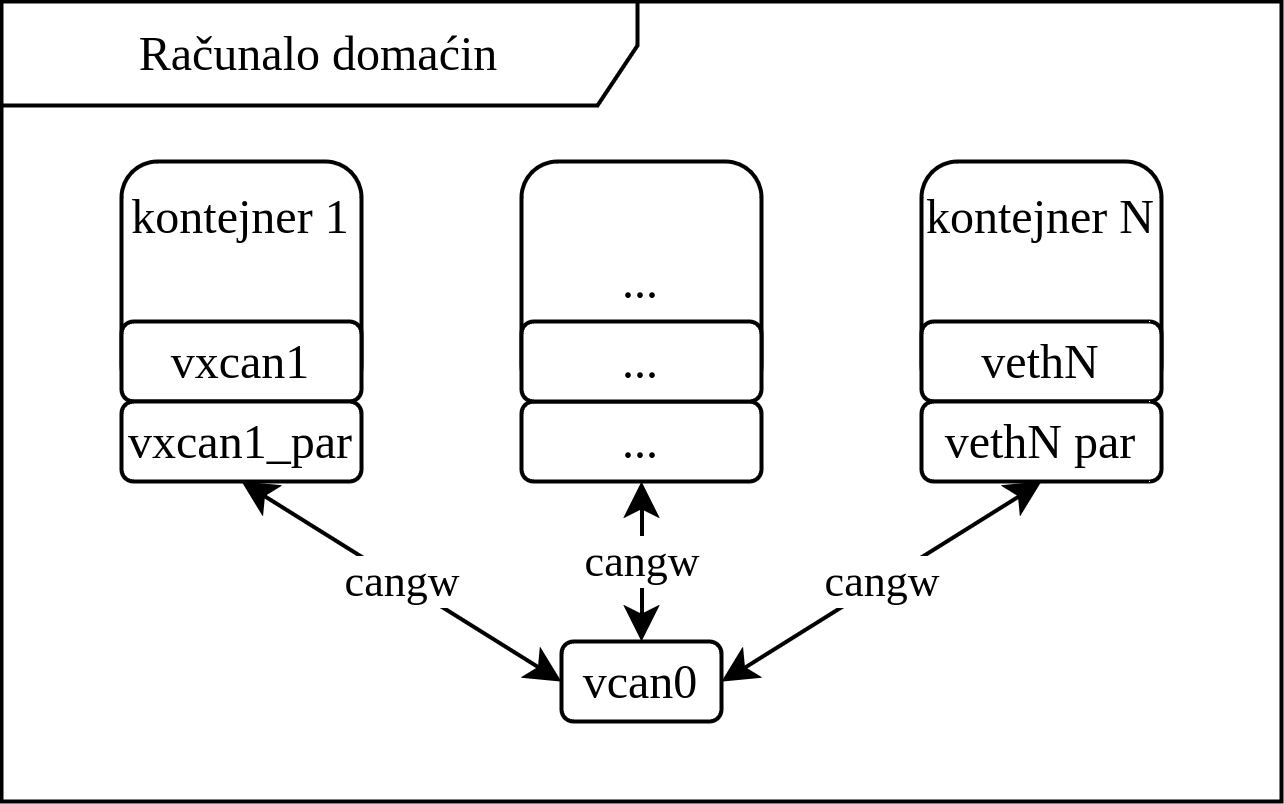
\includegraphics[width=250pt]{vcan_bridge.png}
\caption{Umrežavanje kontejnera korištenjem alata \textit{cangw}}
\label{fig:vcanb}
\end{figure}

\newpage
\begin{lstlisting}[style=terminal, label={lst:vxcan2},caption={Povezivanje mrežnih imenskih prostora alatom \textit{cangw}}]
$ ip link add vxcan1 type vxcan peer name vxcan1_par
$ ip link add vxcan2 type vxcan peer name vxcan2_par
$ ip link add vcan0 type vcan

$ ip link set vxcan1 netns ns1
$ ip link set vxcan2 netns ns2

$ ip a
(...)
9: vxcan1_par@if10: <NOARP> mtu 72 qdisc noop state DOWN group default qlen 1000
    link/can  link-netns ns1
11: vxcan2_par@if12: <NOARP> mtu 72 qdisc noop state DOWN group default qlen 1000
    link/can  link-netns ns2
13: vcan0: <NOARP> mtu 72 qdisc noop state DOWN group default qlen 1000
    link/can 

$ modprobe can_gw max_hops=2

$ cangw -A -s vcan0 -d vxcan1_par -e
$ cangw -A -s vcan0 -d vxcan2_par -e
$ cangw -A -d vcan0 -s vxcan1_par -e
$ cangw -A -d vcan0 -s vxcan2_par -e
$ cangw -L
cangw -A -s vcan0 -d vxcan2_par -e # 0 handled 0 dropped 0 deleted
cangw -A -s vcan0 -d vxcan1_par -e # 0 handled 0 dropped 0 deleted
\end{lstlisting}

\subsection{LibNetwork i udaljeni upravljački programi}
\textit{Docker Engine} omogućava pisanje mrežnih programskih dodataka, kojima je moguće definirati dodatne načine umrežavanja kontejnera. \textit{Docker} podržava nekoliko ugrađenih načina umrežavanja kontejnera, primjerice \textit{Docker bridge}. Ugrađeni načini umrežavanja odnosno njihovi upravljački programi za upravljanje umrežavanjem kontejnera izravno koriste biblioteku \textit{LibNetwork} \cite{libnetwork}.

Pri pisanju mrežnih programskih dodataka, biblioteku nije moguće koristiti izravno, već pisanjem HTTP poslužitelja koji implementira \textit{LibNetwork} protokol za udaljene upravljačke programe \engl{remote driver protocol}. Smatra se da je HTTP poslužitelj implementirao navedeni protokol, ako prihvaća određeni skup HTTP POST zahtjeva s argumentima predanima u JSON formatu. Konkretnije, za definiranje umrežavanja kontejnera bitni su POST zahtjevi na putanje: 
\bigskip
\begin{itemize}
    \item \texttt{/NetworkDriver.CreateNetwork}
    \item \texttt{/NetworkDriver.DeleteNetwork}
    \item \texttt{/NetworkDriver.CreateEndpoint}
    \item \texttt{/NetworkDriver.DeleteEndpoint}
    \item \texttt{/NetworkDriver.Join}
    \item \texttt{/NetworkDriver.Leave}
\end{itemize}

Navedene zahtjeve šalje \textit{Docker Engine} na HTTP poslužitelj dodatka. Zahtjeve \texttt{/Net- workDriver.CreateNetwork} i \texttt{/NetworkDriver.DeleteNetwork} šalje prilikom stvaranja i brisanja mreža kontejnera, zahtjeve \texttt{/NetworkDriver.Create Endpoint} i \texttt{/NetworkDriver.DeleteEndpoint} šalje prije dodavanja i uklanjanja kontejnera iz mreže. Zahtjeve \texttt{/NetworkDriver.Join} i \texttt{/NetworkDriv- er.Leave} šalje prilikom dodavanja i uklanjanja kontejnera iz mreže.

\subsection{Implementacija}
Dodatak, nazvan \textit{dockercan}, implementiran je u programskom jeziku \textit{Go}, korištenjem službenog \textit{Docker} pomoćnog koda za pisanje dodataka \cite{gohelpers}. Dodatno, ovisi o alatima \textit{cangw} i \textit{ip} te modulima jezgre \textit{can\_gw} i \textit{vxcan} za ispravan rad. Dodatak podržava dva načina umrežavanja: centralizirani i \textit{peer-to-peer}. Neovisno o odabranom načinu umrežavanja, dodatak stvara zasebni mrežni imenski prostor za svaku mrežu, koji koristi za skrivanje \textit{cangw} pravila i stvorenih sučelja od korisnika ili natjecatelja. Pri opisivanju oba načina umrežavanja koristi se isti primjer s dvije \textit{dockercan} mreže: mreža "A" sadrži 5 kontejnera, a mreža "B" sadrži 2 kontejnera te ima uključenu opciju stvaranja sučelja za pristup mreži na računalu domaćina. 

\textit{Peer-to-peer} način umrežavanja je jednostavniji za implementaciju, ali koristi $2*\binom{n}{2}$ \textit{cangw} pravila za povezivanje kontejnera. Opis ovog načina umrežavanja, kao i prototip \textit{Docker} dodatka opisan je u \cite{lkml2018candocker}. U ovom načinu umrežavanja, dodatak svakom kontejneru dodjeljuje jedan \textit{vxcan} tunel, gdje je jedan kraj tunela u mrežnom imenskom prostoru kontejnera, a drugi u mrežnom imenskom prostoru njegove mreže (slika \ref{fig:p2p}). Krajevi \textit{vxcan} tunela koji se nalaze u mrežnim prostorima kontejnera, formata su \texttt{ccan\_X}, gdje je \texttt{ccan\_} prefiks, a \texttt{X} neki cijeli broj. \textit{LibNetwork} vodi računa o jedinstvenosti naziva krajeva tunela u istom kontejneru. Primjerice, prema primjeru sa slike \ref{fig:p2p}, kada je kontejner "2" bio dodan u mrežu "A", stvoreno je \textit{vxcan} sučelje \texttt{ccan\_0} u njegovom mrežnom imenskom prostoru. Kada je naknadno dodan u mrežu "B", \textit{LibNetwork} je stvoreno \textit{vxcan} sučelje nazvao \texttt{ccan\_1}, kako bi se izbjegla kolizija u imenima sučelja. Krajevi \textit{vxcan} tunela u mrežnom imenskom prostoru mreža "A" i "B" imenovani su prema formatu \texttt{hcan\_ID}, gdje je \texttt{hcan\_} prefiks, a \texttt{ID} identifikator krajnje točke \engl{endpoint} kontejnera. Krajevi \textit{vxcan} tunela u mrežnom imenskom prostoru mreže, međusobno su povezani \textit{cangw} pravilima. U slučaju mreže "B", odabrana je opcija stvaranja sučelja za pristup mreži na računalu domaćina. Navedena opcija stvara dodatni \textit{vxcan} tunel, čiji je jedan kraj u imenskom prostoru mreže, a drugi kraj u imenskom prostoru računala domaćina. Kraj tunela u imenskom prostoru mreže, povezuje se s \textit{vxcan} tunelima svih kontejnera.

\begin{figure}[htb]
\centering
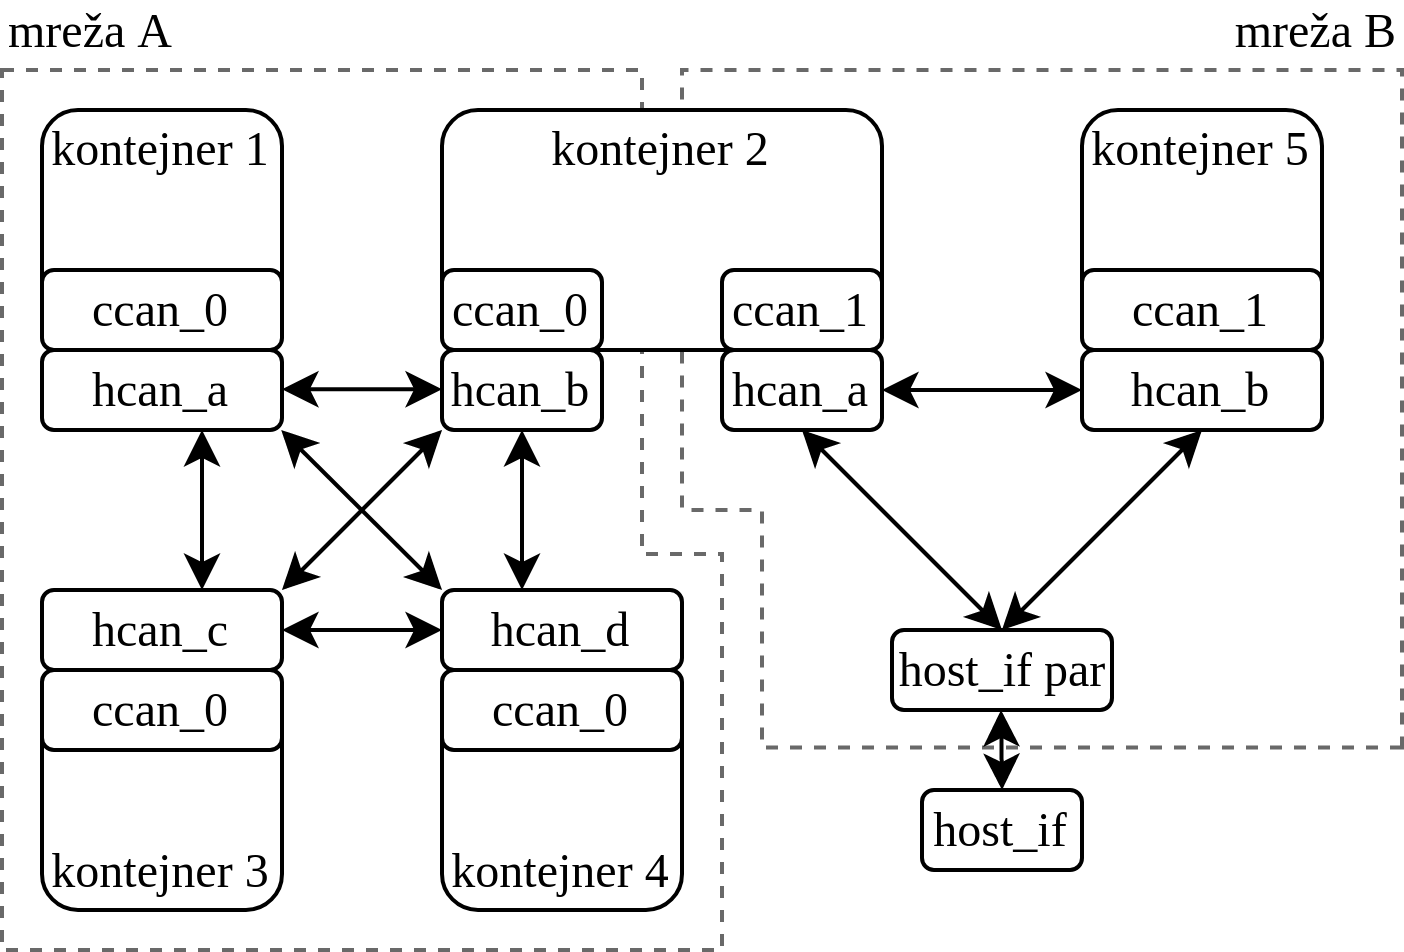
\includegraphics[width=300pt]{necentralizirano_dc.png}
\caption{\textit{Peer-to-peer} umrežavanje}
\label{fig:p2p}
\end{figure}

Centralizirani način umrežavanja koristi optimizaciju opisanu u potpoglavlju \ref{sec:dockercan2} te za umrežavanje $n$ kontejnera koristi $2n$ \textit{cangw} pravila. Kao i u \textit{peer-to-peer} načinu umrežavanja, dodatak za svaki kontejner stvara \textit{vxcan} tunel, gdje jedan kraj tunela postavlja u mrežni imenski prostor mreže, a drugi kraj u mrežni imenski prostor kontejnera. Glavna razlika između dvaju načina povezivanja je što centralizirani način stvara jedno \textit{vcan} sučelje, nazvano \textit{canbus}, u mrežnom imenskom prostoru svake mreže te na njega povezuje krajeve \textit{vxcan} tunela svakog kontejnera, kao i tunela prema imenskom prostoru računala domaćina, korištenjem \textit{cangw} pravila (slika \ref{fig:centralised}). Na centralno \textit{vcan} sučelje jednostavno je spojiti i \textit{SocketCAN} sučelje prema CAN sklopovlju, čime se omogućava spajanje virtualnih i fizičkih CAN sabirnica. 
\newpage
\begin{figure}[htb]
\centering
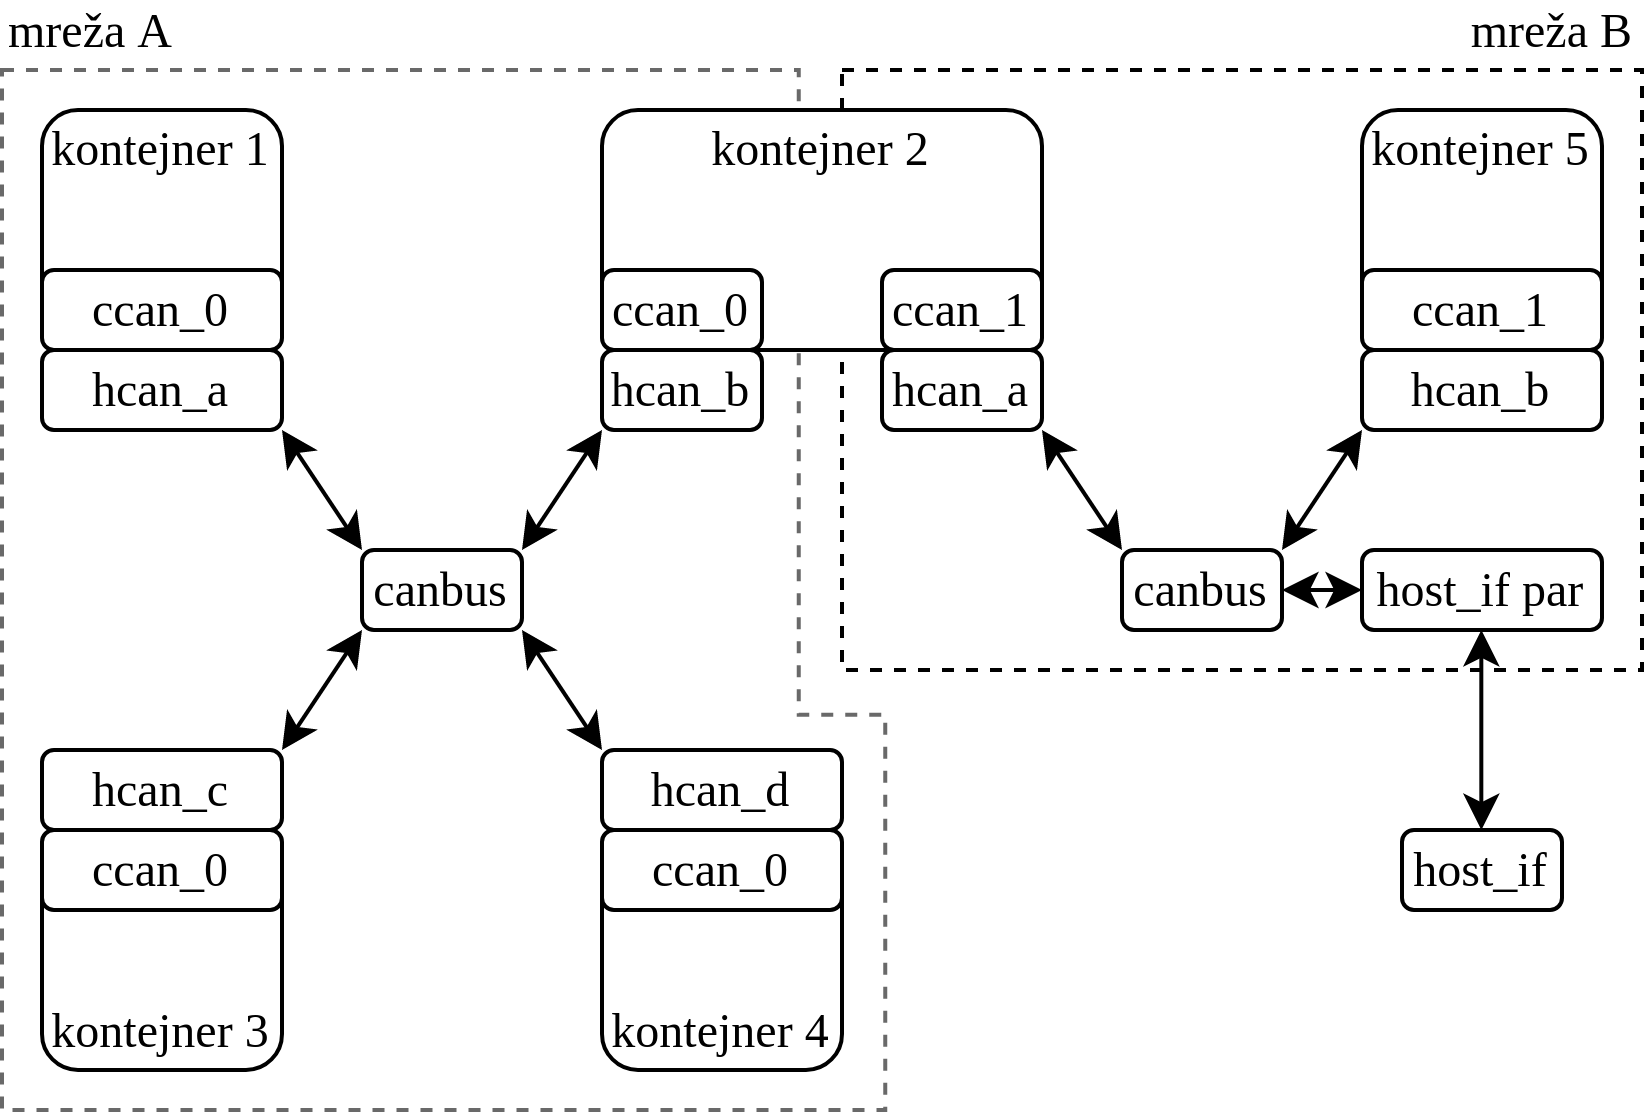
\includegraphics[width=300pt]{centralizirano_dc.png}
\caption{Centralizirano umrežavanje}
\label{fig:centralised}
\end{figure}
\subsection{Korištenje}
Dodatak je moguće učitati na tri načina:
\begin{itemize}
    \item pokretanjem kroz naredbeni redak
    \item kao \textit{Systemd} servis
    \item instalacijom kroz sustav \textit{Docker} dodataka
\end{itemize}

Pokretanjem kroz naredbeni redak, dodatak radi kao HTTP poslužitelj na TCP pristupu 4343. U slučaju učitavanja dodatka kao \textit{Systemd} servisa s konfiguracijskom datotekom prikazanom u ispisu \ref{lst:systemd}, dodatak radi kao HTTP poslužitelj na TCP pristupu 5555. Naposljetku, dodatak se može izgraditi za instalaciju kroz sustav \textit{Docker}dodataka, pri čemu se pokreće u posebnom načinu u kojem se za komunikaciju s \textit{Docker Engine} procesom ne koristi HTTP poslužitelj već \textit{Unix} domenski priključak \engl{Unix domain socket}. U sva tri navedena slučaja, službeni pomoćni kod za pisanje \textit{Docker} dodataka automatski stvara potrebne specifikacijske datoteke u direktorijima \texttt{/etc/docker/plugins} i \texttt{/usr/lib/docker/plugins}.

Pri stvaranju \textit{dockercan} mreža korištenjem \textit{Docker} sučelja za naredbeni redak (engl. \textit{command line interface}, CLI) ili putem \texttt{compose.yml} datoteka moguće je specificirati tri opcije. Opcija \texttt{centralised} određuje koji način umrežavanja će dodatak koristiti, opcija \texttt{canfd} će omogućiti slanje CAN-FD poruka kroz stvorenu mrežu, a opcija \texttt{host\_if} omogućava specificiranje imena sučelja za pristup mreži koje će biti stvoreno na računalu domaćina. Primjeri korištenja dodatka putem \textit{Docker} CLI-a i \texttt{compose.yml} datoteke prikazani su u ispisima \ref{lst:cli1} i \ref{lst:compose1}.


\newpage
\begin{lstlisting}[style=terminal, label={lst:systemd},caption={Konfiguracijska datoteka Systemd servisa}]
[Unit]
Description=Dockercan network plugin
Before=docker.service
After=network.target
Requires=docker.service

[Service]
User=root
ExecStart=/usr/lib/docker/dockercan_remote -addr 127.0.0.1:5555

[Install]
WantedBy=multi-user.target

\end{lstlisting}
\begin{lstlisting}[style=terminal, label={lst:cli1},caption={Korištenje dodatka kroz \textit{Docker} CLI}]
$ docker network create -o centralised=true -o canfd=true -o host_if=dcan1 --driver dockercan sabirnica1
\end{lstlisting}

\begin{lstlisting}[style=terminal, label={lst:compose1},caption={Primjer \texttt{compose.yml} datoteke}]
services:
  ECM:
    image: alpine
    networks: [ pogonskisklop ]
  
  TCU:
    image: alpine
    networks: [ pogonskisklop ]

networks:
  pogonskisklop:
    driver: dockercan
    driver_opts:
      centralised: "false"
      canfd:       "true"
      host_if:     "dcan1"
\end{lstlisting}
\newpage
\section{Generatorska skripta}
U sklopu sustava za izradu CTF zadataka, napisana je jednostavna skripta za generiranje početnog stabla direktorija i \texttt{compose.yml} datoteke za pokretanje zadatka. Pokretanje i početni izbornik skripte prikazan je ispisom \ref{lst:dockar1}.  
\begin{lstlisting}[style=terminal, label={lst:dockar1},caption={Glavni izbornik generatorske skripte}]
$ mkdir out
$ python3 generate.py out

   ___  ____  _______ _____   ___ 
  / _ \/ __ \/ ___/ //_/ _ | / _ \
 / // / /_/ / /__/ ,< / __ |/ , _/
/____/\____/\___/_/|_/_/ |_/_/|_|     
    

    Select option:

    1) Add CAN bus
    2) Add ECU
    3) Done
    4) Exit
    
Enter choice [1-4]:
\end{lstlisting}
\subsection{Primjer generiranja projekta}
Za potrebe primjera, cilj je generirati projekt s dvije CAN sabirnice, za ECU-ove domena pogonskog sklopa i kabine. Na sabirnicu domene kabine potrebno je spojiti ECU ploče s instrumentima, koji se temelji na predlošku programa ECU-a. Uz to, potrebno mu je dodijeliti vizualnu komponentu, odnosno povezati ga s TUI-jem ploče s instrumentima. Sabirnica domene kabine mora biti dostupna udaljeno putem \textit{cannellonni} tunela te lokalno putem \textit{SocketCAN} sučelja na računalu domaćinu. Na sabirnicu domene pogonskog sklopa potrebno je povezati ECU motora, koji se temelji na predlošku programa ECU-a. Sabirnica domene pogonskog sklopa ne smije biti dostupna lokalno niti udaljeno, već samo putem poveznika koji spaja obje sabirnice. Na obje sabirnice potrebno je generirati šum.

Prilikom dodavanja sabirnice nude se opcije: korištenja protokola CAN-FD umjesto klasičnog CAN-a, dodavanja \textit{cannelloni} kontejnera za udaljeno povezivanje, dodavanja lokalnog \textit{SocketCAN} sučelja te generiranja šuma na sabirnici. Dodavanje sabirnice domene kabine prikazano je ispisom \ref{lst:dockar2}.
\bigskip
\begin{lstlisting}[style=terminal, label={lst:dockar2},caption={Dodavanje sabirnice}]
Enter choice [1-4]: 1
Enter bus name:  kabina
[dockercan] Connect host to this bus over vcan interface?[y/n]: y
Enter interface name: ctf_ulaz
[dockercan] Use CAN FD?[y/n]: n
Add random CAN frame generation to this bus?[y/n]: y
Attach cannelloni container?[y/n]: y
\end{lstlisting}

Prilikom dodavanja ECU-a nude se opcije korištenja predloška ECU programa te povezivanja na TUI ploče s instrumentima. Naposljetku je potrebno odabrati sabirnice na koje će ECU biti povezan. Ispisom \ref{lst:dockar3} prikazano je dodavanje ECU-a ploče s instrumentima kojem treba dodijeliti TUI ploče s instrumentima te dodavanje poveznika kojeg treba povezati s obje sabirnice.
\bigskip
\begin{lstlisting}[style=terminal, label={lst:dockar3},caption={Dodavanje ECU-a}]
Enter choice [1-4]: 2
Enter ECU name: poveznik
Use ECU template?[y/n]: n
Connect ECU to IC-TUI?[y/n]: n
Connect ECU to which buses? (e.g. 1,3)
 1) pogon
 2) kabina

Enter choice:  1,2

(...)

Enter choice [1-4]: 2
Enter ECU name: ic-ecu
Use ECU template?[y/n]: y
Connect ECU to IC-TUI?[y/n]: y
Connect ECU to which buses? (e.g. 1,3)
 1) pogon
 2) kabina

Enter choice:  2
\end{lstlisting}
\newpage

Nakon svakog dodanog elementa ispisuje se izgled trenutne arhitekture, a odabirom treće opcije skripta generira stablo direktorija i početni kod zadatka (ispis \ref{lst:dockar4}). U \texttt{compose.yml} datoteci kontejner ECU ploče s instrumentima i TUI-ja stavljeni su u zasebnu \textit{Docker bridge} mrežu, kako bi se omogućila komunikacija putem TUI-jevog HTTP API-ja. Uz navedeno, \textit{cannelloni} kontejneru je otvoren TCP pristup 20000, odnosno pretpostavljeni pristup za \textit{cannelloni} TCP poslužitelj. Za svaki idući dodani \textit{cannelloni} kontejner, pristup se inkrementira. Za ECU-ove za koje je odabrana opcija korištenja predloška, generiran je početni kod u odgovarajućim direktorijima te su u \texttt{compose.yml} datoteci definiranje putanje izgradnje kontejnera. 
\bigskip
\begin{lstlisting}[style=terminal, label={lst:dockar4},caption={Završetak postupka generacije projekta}]
 ========= NETWORK LAYOUT =========
 
pogon           kabina          
│               │               
├ noise_gen     ├ noise_gen     
│               │               
├ ecm           ├ cannelloni    
│               │               
├ poveznik      ├ poveznik      
│               │               
│               ├ ic-ecu               

 ========= NETWORK LAYOUT ========= 

    Select option:

    1) Add CAN bus
    2) Add ECU
    3) Done
    4) Exit
    
Enter choice [1-4]: 3

$ ls out
cangen  cannelloni  compose.yml  ecm  ic-ecu  ic-tui0
\end{lstlisting}
\newpage
\subsection{Mogućnosti pristupa za natjecatelje}
U kontekstu generiranog projekta iz prethodnog poglavlja, postoji nekoliko načina omogućavanja udaljenog i lokalnog pristupa. Ukoliko natjecatelj ima lokalni pristup zadatku, potrebno mu je ograničiti mogućnosti stvaranjem korisnika s niskom razinom privilegija, kako bi interakcija bila ograničena na korištenje dopuštenih alata na \textit{SocketCAN} sučelju računala domaćina. Uz to, lokalni prikaz TUI-ja, moguće je ostvariti korištenjem naredbe \texttt{docker attach} na TUI kontejneru, u slučaju da je TUI pokrenut bez zastavice "-ssh". Suprotno, u slučaju da je TUI pokrenut u SSH načinu rada, potrebno je korisniku dozvoliti spajanje na lokalni SSH server TUI kontejnera.

Ako natjecatelj pristupa s udaljenog računala, potrebno mu je pružiti upute i podatke za spajanje na \textit{cannelloni} TCP server, kako bi imao pristup nekoj od CAN sabirnica. Za udaljeni prikaz TUI-ja, dovoljno ga je pokrenuti u SSH načinu rada te korisniku dati podatke za spajanje. Alternativa ovom načinu udaljenog pristupa je primjenjivanje svih prethodno navedenih mjera za lokalni pristup te omogućavanje SSH pristupa putem korisnika s niskom razinom privilegija.
\section{Zadaci}
U sklopu ovog rada izrađena su tri zadatka koji demonstriraju ranjivosti i ranjive implementacije protokola CAN i UDS. Konkretnije, zadaci demonstriraju iskorištavanje UDS servisa \texttt{ReadMemoryByAddress}, iskorištavanje ranjive implementacije UDS \texttt{SecurityAccess} servisa te napad lažiranjem putem protokola CAN. Zadaci su namijenjeni za rješavanje korištenjem alata \textit{caringcaribou}, \textit{Scapy} i \textit{can-utils} paketa \cite{caringcaribou, scapy}. U nastavku je opisan tijek rješavanja zadataka.

\subsection{Iskorištavanje UDS servisa ReadMemoryByAddress}
Natjecatelju je na početku zadatka dana informacija da ECU koristi procesor s 32-bitnim memorijskim adresiranjem. Natjecatelj dobiva pristup CAN sabirnici na koju je povezan ECU s UDS poslužiteljem. Korištenjem alata \textit{caringcaribou} odnosno njegovog modula za otkrivanje UDS poslužitelja, natjecatelj saznaje ISO-TP adresu poslužitelja. Potom natjecatelj ponovo koristi alat \textit{caringcaribou} za skeniranje dostupnih UDS servisa te pronalazi servis \texttt{ReadMemoryByAddress}. Korištenjem informacije o duljini memorijskih adresa, napadač mora sastaviti skriptu kojom će pročitati cjelokupnu memoriju ECU-a. Skriptu je moguće napisati korištenjem biblioteke \textit{Scapy}, \textit{can-utils} alata ili izravnim korištenjem \textit{Berkley socket} API-ja otvaranjem \textit{socketa} nad \textit{SocketCAN} sučeljem (ispis \ref{lst:rmbas}). Nakon što je pročitao memoriju ECU-a, zastavicu može pronaći traženjem niza znakova koji odgovara danom formatu zastavice u pročitanim podacima.
\bigskip
\begin{lstlisting}[language=Python, label={lst:rmbas},caption={\textit{Scapy} skripta za čitanje cjelokupne memorije ECU-a}]
memorySizeLen = 1
memoryAddressLen = 4
data = b""
addr = 0x0
size = 0xFF

while True:
    pckt = sock.sr1(UDS() / UDS_RMBA(memorySizeLen=memorySizeLen,
                                     memoryAddressLen=memoryAddressLen,
                                     memorySize1=size,
                                     memoryAddress4=addr),
                    verbose=False)
    if isinstance(pckt.payload, UDS_NR):
        break
    if isinstance(pckt.payload, UDS_RMBAPR):
        data += pckt.dataRecord
    print(f"Addr: {addr}", end="\r")
    addr += size

with open("binary", "wb") as f:
    f.write(data)
\end{lstlisting}
\subsection{Iskorištavanje ranjive implementacije UDS SecurityAccess servisa}
Kao i u prethodnom zadatku, natjecatelj mora iskoristiti alat \textit{caringcaribou} u svrhu otkrivanja ISO-TP adrese UDS poslužitelja te dostupnih UDS servisa, odnosno servisa \texttt{SecurityAccess}, \texttt{ReadMemoryByAddress}, \texttt{ReadDataByIdentifier}.Kroz pokušaje komunikacije sa servisima, natjecatelj mora zaključiti da je servis \texttt{ReadMe- moryByAddress} zaštićen servisom \texttt{SecurityAccess}, ali da \texttt{ReadDataByIde- ntifier} servis nije. Korištenjem funkcije \texttt{dump\_dids} alata \textit{caringcaribou}, natjecatelj može iščitati vrijednosti iz identifikatora 9 i 21 u heksadekadskom formatu (ispis \ref{lst:ccdid}). Pretvaranjem navedenih vrijednosti u ASCII znakove, natjecatelj otkriva broj šasije vozila odnosno prvu zastavicu te niz znakova "SHA-512". Natjecatelj potom treba zaključiti da \texttt{SecurityAccess} neispravno koristi algoritam SHA-512 kao \textit{seed-and-key} algoritam.
\bigskip
\begin{lstlisting}[style=terminal, label={lst:ccdid},caption={Dodavanje ECU-a}]
$ caringcaribou uds dump_dids --max_did 0x25 0x100 0x101

(...)

Identified DIDs:
DID    Value (hex)
0x0009 335657465837415432444d363034343934
0x0021 5348412d353132

\end{lstlisting}

Naposljetku, kako bi ostvario pristup servisu \texttt{ReadMemoryByAddress}, natjecatelj treba zatražiti \textit{seed} vrijednost slanjem \texttt{SecurityAccess} zahtjeva te izračunati ključ odnosno SHA-512 sažetak dobivene \textit{seed} vrijednosti. Nakon autorizacije, natjecatelj treba isčitati sadržaj memorije ECU-a te u njoj pronaći zastavicu, kao u prethodnom zadatku. 

\subsection{Napad lažiranjem putem protokola CAN}
Posljednji zadatak sastoji se od poveznika i ECU-a ploče s instrumentima te pripadajućeg TUI-ja. Poveznik podržava UDS servis \texttt{RoutineControl}, a pokretanjem bilo koje od rutina, poveznik počinje slati testni niz CAN poruka. Testni niz poruka redom pali statusne LED diode na ploči s instrumetima te inkrementira prikazanu brzinu od 0 km/h do 170 km/h. U svrhu otežavanja zadatka, na sabirnici se konstantno generiraju nasumične CAN poruke. Uvjet za prikaz zastavice na TUI-ju je postići brzinu preko 230km/h i upaliti pokazivače smjera.

Natjecatelj treba iskoristiti mogućnost višestrukog pokretanja rutine kako bi reverznim inženjeringom CAN prometa shvatio koje okvire treba modificirati i ponovno poslati, kako bi ispunio uvjet za prikaz zastavice. 

\chapter{Zaključak}
Implementirani sustav pruža robusan način za stvaranje CTF zadataka u području sigurnosti automobila. \textit{Docker} dodatkom omogućeno je pouzdano i prilagodljivo umrežavanje kontejnera putem virtualnih CAN sučelja i tunela. Predloškom programa ECU-a olakšana je implementacija CTF zadataka, pružanjem prilagodljive programske arhitekture za implementaciju aplikacijske logike u kontekstu protokola CAN, UDS i XCP. Uz to, demonstrirana je mogućnost povezivanja predloška s dodatnim programskim proširenjima putem \textit{Docker bridge} mreža. Izrađen je primjer programskog proširenja u obliku vizualne komponente, odnosno TUI-ja ploče s instrumentima. Sustav je objedinjen generatorskom skriptom koja omogućava sastavljanje arhitekture CTF zadatka, kao i generiranje početnog koda te \textit{Docker Compose} konfiguracijske datoteke za jednostavnije postavljanje zadatka. Definirani su načini omogućavanja udaljenog i lokalnog pristupa zadacima. Napravljen je pregled E/E arhitekture modernih automobila kao i pregled postojećih istraživanja sigurnosti u posljednjem i ovom desetljeću. Analizirani su postojeći edukativni materijali u području kibernetičke sigurnosti automobila te su izrađena su tri CTF zadatka koji demonstriraju ranjivosti protokola CAN i UDS, ali i služe kao smjernice za izradu novih CTF zadataka korištenjem implementiranog sustava.

Nedostatak implementiranog sustava je nemogućnost simuliranja napada na fizičkom sloju. S obzirom na to da je sustav implementiran prvenstveno programski, nije moguće simulirati napade poput \textit{bus-off} napada koji iskorištava interne brojače grešaka CAN primopredajnika, kao ni DoS napade koji iskorištavaju mehanizam arbitraže sabirnice. S druge strane, implementacija \textit{Docker} dodatka za umrežavanje korištenjem \textit{SocketCAN} paketa, omogućava povezivanje CAN sklopovlja na virtualnu mrežu, čime je moguće zaobići neke od navedenih nedostataka. 

U daljnjem radu treba formalizirati načine povezivanja sklopovlja u virtualnu mrežu, nadogradnjom generatorske skripte ili izradom aplikacije koja će dodatno objediniti sve implementirane komponente sustava. Potrebno je i izraditi dodatne konfigurabilne ECU kontejnere, poput kontejnera poveznika koji bi omogućio povezivanje više sabirnica i filtriranje CAN poruka između njih. U predlošku programa ECU-a, potrebno je unaprijediti razrede za implementaciju XCP i UDS logike, dodavanjem implementabilnih sučelja za formalnu implementaciju određenih servisa. Naposljetku, iako je implementirani sustav dostatan za simuliranje aplikacijske logike klasičnih ECU-ova kao i ranjivosti protokola UDS, XCP i CAN, potrebno je u daljnjim iteracijama staviti naglasak i na simuliranje napada na sustave zabave.       



\bibliography{literatura}
\bibliographystyle{fer}


\begin{sazetak}
Ovaj rad opisuje implementaciju proširivog sustava za stvaranje CTF zadataka specifičnih za sustave upravljanja i
zabave u automobilima. Napravljen je generalni pregled E/E arhitekture modernih automobila, tipova arhitektura kao i najčešćih komunikacijskih, dijagnostičkih i kalibracijskih protokola. Uz navedeno, razmotrena su postojeća istraživanja sigurnosti te stvarni napadi na sustave automobila, ali i napadi na same protokole kojima sustavi automobila komuniciraju. Analizirani su postojeći materijali za obuku sadašnjih ili budućih stručnjaka sigurnosti te je sukladno njihovim prednostima i nedostacima razvijen novi proširivi sustav za stvaranje CTF zadataka. S pomoću novog sustava razvijena su tri zadatka koji demonstriraju moguće napade na protokole CAN i UDS.

\kljucnerijeci{UDS, CAN, CTF, kibernetička sigurnost, automobilska indrustrija, vozila, simulator}
\end{sazetak}

\engtitle{Extensible system for creating CTF tasks specific to automotive control and infotainment systems}
\begin{abstract}
This paper describes the implementation of an extensible system for creating CTF tasks specific to automotive control and infotainment systems. It provides a general overview of the E/E architecture of modern cars, types of architectures, as well as the most common communication, diagnostic, and calibration protocols. In addition, an overview of existing security research and actual attacks on car systems, as well as attacks on the protocols used by car systems, is provided. Existing training materials for current or future security experts are analyzed, and based on their advantages and disadvantages, a new extensible system for creating CTF tasks has been developed. Using the new system, three tasks were developed that demonstrate possible attacks on the CAN and UDS protocols.

\keywords{UDS, CAN, CTF, cybersecurity, automotive, vehicles, simulator}
\end{abstract}

\end{document}
